\documentclass{article}
\usepackage{amsmath}
\usepackage{graphicx}
\usepackage[margin=2.2cm]{geometry}
\begin{document}
\section*{SK Matrix-Model Contributions for All L=2 Topologies}
External assignment (by external-propagator appearance): $\phi_r^1(x_1)\,\phi_a^1(x_2)\,\phi_r^2(x_3)\,\phi_a^2(x_4)$, with $x_1=(t,\mathbf{x})$, $x_2=(0,\mathbf{0})$, $x_3=(t,\mathbf{x})$, $x_4=(0,\mathbf{0})$.
Translation table used: same-fold $G_{rr}\to G_K=\frac12(G^>+G^<)$, $G_{ra}\to G_R$, $G_{ar}\to G_A$, $G_{aa}\to 0$; cross-fold $G^{12}_{rr}\to G^<$, $G^{21}_{rr}\to G^>$, and any cross-fold propagator with an $a$ endpoint vanishes.
Contour ordering convention: contour $(2)$ is later than contour $(1)$, matching \texttt{contour\_ra\_translation.txt}.
Each term carries explicit net matrix-size factor ${N_c}^{p-4}$ (raw loop count $p$ minus the overall $1/N^4$ normalization).
\section*{Topology 1 (FeynArts Topology 2)}
\begin{center}

\includegraphics[width=0.28\textwidth]{generated/L2/images/topology1.pdf}
\end{center}
\noindent Parsed propagators: 8. Internal vertices: 3. Internal half-edges: 12.\\
\noindent Assignments checked: 32768. Surviving (nonzero vertex weight): 4096.\\
\noindent Raw $N_c$ power: 0. Net power in $C(t)$: -4.
\noindent Explicit surviving terms:
\begin{equation*}
\mathcal{T}_{1,1} = 128 i g_{2}^{3}\,N_c^{-4}\,G^<\left(z_{1},z_{3}\right) \, G^<\left(z_{2},z_{3}\right) \, G_A\left(x_2,z_{2}\right) \, G_A\left(x_4,z_{3}\right) \, G_A\left(z_{2},z_{1}\right) \, G_K\left(x_1,z_{1}\right) \, G_R\left(x_3,z_{3}\right) \, G_R\left(z_{2},z_{1}\right)
\end{equation*}
\begin{equation*}
\mathcal{T}_{1,2} = 128 i g_{2}^{3}\,N_c^{-4}\,G^<\left(z_{1},z_{3}\right) \, G^<\left(z_{2},z_{3}\right) \, G_A\left(x_2,z_{2}\right) \, G_A\left(x_4,z_{3}\right) \, G_A\left(z_{2},z_{1}\right) \, G_K\left(z_{2},z_{1}\right) \, G_R\left(x_1,z_{1}\right) \, G_R\left(x_3,z_{3}\right)
\end{equation*}
\section*{Topology 2 (FeynArts Topology 2)}
\begin{center}

\includegraphics[width=0.28\textwidth]{generated/L2/images/topology2.pdf}
\end{center}
\noindent Parsed propagators: 8. Internal vertices: 3. Internal half-edges: 12.\\
\noindent Assignments checked: 32768. Surviving (nonzero vertex weight): 4096.\\
\noindent Raw $N_c$ power: 0. Net power in $C(t)$: -4.
\[\text{No surviving SK contributions for this topology.}\]
\section*{Topology 3 (FeynArts Topology 2)}
\begin{center}

\includegraphics[width=0.28\textwidth]{generated/L2/images/topology3.pdf}
\end{center}
\noindent Parsed propagators: 8. Internal vertices: 3. Internal half-edges: 12.\\
\noindent Assignments checked: 32768. Surviving (nonzero vertex weight): 4096.\\
\noindent Raw $N_c$ power: 0. Net power in $C(t)$: -4.
\[\text{No surviving SK contributions for this topology.}\]
\section*{Topology 4 (FeynArts Topology 2)}
\begin{center}

\includegraphics[width=0.28\textwidth]{generated/L2/images/topology4.pdf}
\end{center}
\noindent Parsed propagators: 8. Internal vertices: 3. Internal half-edges: 12.\\
\noindent Assignments checked: 32768. Surviving (nonzero vertex weight): 4096.\\
\noindent Raw $N_c$ power: 0. Net power in $C(t)$: -4.
\[\text{No surviving SK contributions for this topology.}\]
\section*{Topology 5 (FeynArts Topology 2)}
\begin{center}

\includegraphics[width=0.28\textwidth]{generated/L2/images/topology5.pdf}
\end{center}
\noindent Parsed propagators: 8. Internal vertices: 3. Internal half-edges: 12.\\
\noindent Assignments checked: 32768. Surviving (nonzero vertex weight): 4096.\\
\noindent Raw $N_c$ power: 0. Net power in $C(t)$: -4.
\[\text{No surviving SK contributions for this topology.}\]
\section*{Topology 6 (FeynArts Topology 2)}
\begin{center}

\includegraphics[width=0.28\textwidth]{generated/L2/images/topology6.pdf}
\end{center}
\noindent Parsed propagators: 8. Internal vertices: 3. Internal half-edges: 12.\\
\noindent Assignments checked: 32768. Surviving (nonzero vertex weight): 4096.\\
\noindent Raw $N_c$ power: 0. Net power in $C(t)$: -4.
\noindent Explicit surviving terms:
\begin{equation*}
\mathcal{T}_{6,1} = 128 i g_{2}^{3}\,N_c^{-4}\,G^>\left(z_{2},z_{1}\right) \, G^>\left(z_{3},z_{1}\right) \, G_A\left(x_2,z_{1}\right) \, G_A\left(x_4,z_{3}\right) \, G_A\left(z_{3},z_{2}\right) \, G_K\left(x_3,z_{2}\right) \, G_R\left(x_1,z_{1}\right) \, G_R\left(z_{3},z_{2}\right)
\end{equation*}
\begin{equation*}
\mathcal{T}_{6,2} = 128 i g_{2}^{3}\,N_c^{-4}\,G^>\left(z_{2},z_{1}\right) \, G^>\left(z_{3},z_{1}\right) \, G_A\left(x_2,z_{1}\right) \, G_A\left(x_4,z_{3}\right) \, G_A\left(z_{3},z_{2}\right) \, G_K\left(z_{3},z_{2}\right) \, G_R\left(x_1,z_{1}\right) \, G_R\left(x_3,z_{2}\right)
\end{equation*}
\section*{Topology 7 (FeynArts Topology 2)}
\begin{center}

\includegraphics[width=0.28\textwidth]{generated/L2/images/topology7.pdf}
\end{center}
\noindent Parsed propagators: 8. Internal vertices: 3. Internal half-edges: 12.\\
\noindent Assignments checked: 32768. Surviving (nonzero vertex weight): 4096.\\
\noindent Raw $N_c$ power: 1. Net power in $C(t)$: -3.
\noindent Explicit surviving terms:
\begin{equation*}
\mathcal{T}_{7,1} = 64 i g_{2}^{3}\,N_c^{-3}\,G^<\left(z_{1},z_{2}\right) \, G^<\left(z_{1},z_{3}\right) \, G_A\left(x_2,z_{1}\right) \, G_A\left(x_4,z_{2}\right) \, G_A\left(z_{2},z_{3}\right) \, G_A\left(z_{3},z_{3}\right) \, G_K\left(x_3,z_{2}\right) \, G_R\left(x_1,z_{1}\right)
\end{equation*}
\begin{equation*}
\mathcal{T}_{7,2} = 64 i g_{2}^{3}\,N_c^{-3}\,G^<\left(z_{1},z_{2}\right) \, G^<\left(z_{1},z_{3}\right) \, G_A\left(x_2,z_{1}\right) \, G_A\left(x_4,z_{2}\right) \, G_A\left(z_{2},z_{3}\right) \, G_K\left(x_3,z_{2}\right) \, G_R\left(x_1,z_{1}\right) \, G_R\left(z_{3},z_{3}\right)
\end{equation*}
\begin{equation*}
\mathcal{T}_{7,3} = 64 i g_{2}^{3}\,N_c^{-3}\,G^<\left(z_{1},z_{2}\right) \, G^<\left(z_{1},z_{3}\right) \, G_A\left(x_2,z_{1}\right) \, G_A\left(x_4,z_{2}\right) \, G_A\left(z_{3},z_{3}\right) \, G_K\left(z_{2},z_{3}\right) \, G_R\left(x_1,z_{1}\right) \, G_R\left(x_3,z_{2}\right)
\end{equation*}
\begin{equation*}
\mathcal{T}_{7,4} = 64 i g_{2}^{3}\,N_c^{-3}\,G^<\left(z_{1},z_{2}\right) \, G^<\left(z_{1},z_{3}\right) \, G_A\left(x_2,z_{1}\right) \, G_A\left(x_4,z_{2}\right) \, G_K\left(z_{2},z_{3}\right) \, G_R\left(x_1,z_{1}\right) \, G_R\left(x_3,z_{2}\right) \, G_R\left(z_{3},z_{3}\right)
\end{equation*}
\begin{equation*}
\mathcal{T}_{7,5} = 64 i g_{2}^{3}\,N_c^{-3}\,G^<\left(z_{1},z_{2}\right) \, G^<\left(z_{1},z_{3}\right) \, G_A\left(x_2,z_{1}\right) \, G_A\left(x_4,z_{2}\right) \, G_K\left(z_{3},z_{3}\right) \, G_R\left(x_1,z_{1}\right) \, G_R\left(x_3,z_{2}\right) \, G_R\left(z_{2},z_{3}\right)
\end{equation*}
\begin{equation*}
\mathcal{T}_{7,6} = 64 i g_{2}^{3}\,N_c^{-3}\,G^<\left(z_{1},z_{2}\right) \, G^>\left(z_{2},z_{3}\right) \, G_A\left(x_2,z_{1}\right) \, G_A\left(x_4,z_{2}\right) \, G_A\left(z_{1},z_{3}\right) \, G_A\left(z_{3},z_{3}\right) \, G_K\left(x_1,z_{1}\right) \, G_R\left(x_3,z_{2}\right)
\end{equation*}
\begin{equation*}
\mathcal{T}_{7,7} = 64 i g_{2}^{3}\,N_c^{-3}\,G^<\left(z_{1},z_{2}\right) \, G^>\left(z_{2},z_{3}\right) \, G_A\left(x_2,z_{1}\right) \, G_A\left(x_4,z_{2}\right) \, G_A\left(z_{1},z_{3}\right) \, G_K\left(x_1,z_{1}\right) \, G_R\left(x_3,z_{2}\right) \, G_R\left(z_{3},z_{3}\right)
\end{equation*}
\begin{equation*}
\mathcal{T}_{7,8} = 64 i g_{2}^{3}\,N_c^{-3}\,G^<\left(z_{1},z_{2}\right) \, G^>\left(z_{2},z_{3}\right) \, G_A\left(x_2,z_{1}\right) \, G_A\left(x_4,z_{2}\right) \, G_A\left(z_{3},z_{3}\right) \, G_K\left(z_{1},z_{3}\right) \, G_R\left(x_1,z_{1}\right) \, G_R\left(x_3,z_{2}\right)
\end{equation*}
\begin{equation*}
\mathcal{T}_{7,9} = 64 i g_{2}^{3}\,N_c^{-3}\,G^<\left(z_{1},z_{2}\right) \, G^>\left(z_{2},z_{3}\right) \, G_A\left(x_2,z_{1}\right) \, G_A\left(x_4,z_{2}\right) \, G_K\left(z_{1},z_{3}\right) \, G_R\left(x_1,z_{1}\right) \, G_R\left(x_3,z_{2}\right) \, G_R\left(z_{3},z_{3}\right)
\end{equation*}
\begin{equation*}
\mathcal{T}_{7,10} = 64 i g_{2}^{3}\,N_c^{-3}\,G^<\left(z_{1},z_{2}\right) \, G^>\left(z_{2},z_{3}\right) \, G_A\left(x_2,z_{1}\right) \, G_A\left(x_4,z_{2}\right) \, G_K\left(z_{3},z_{3}\right) \, G_R\left(x_1,z_{1}\right) \, G_R\left(x_3,z_{2}\right) \, G_R\left(z_{1},z_{3}\right)
\end{equation*}
\section*{Topology 8 (FeynArts Topology 2)}
\begin{center}
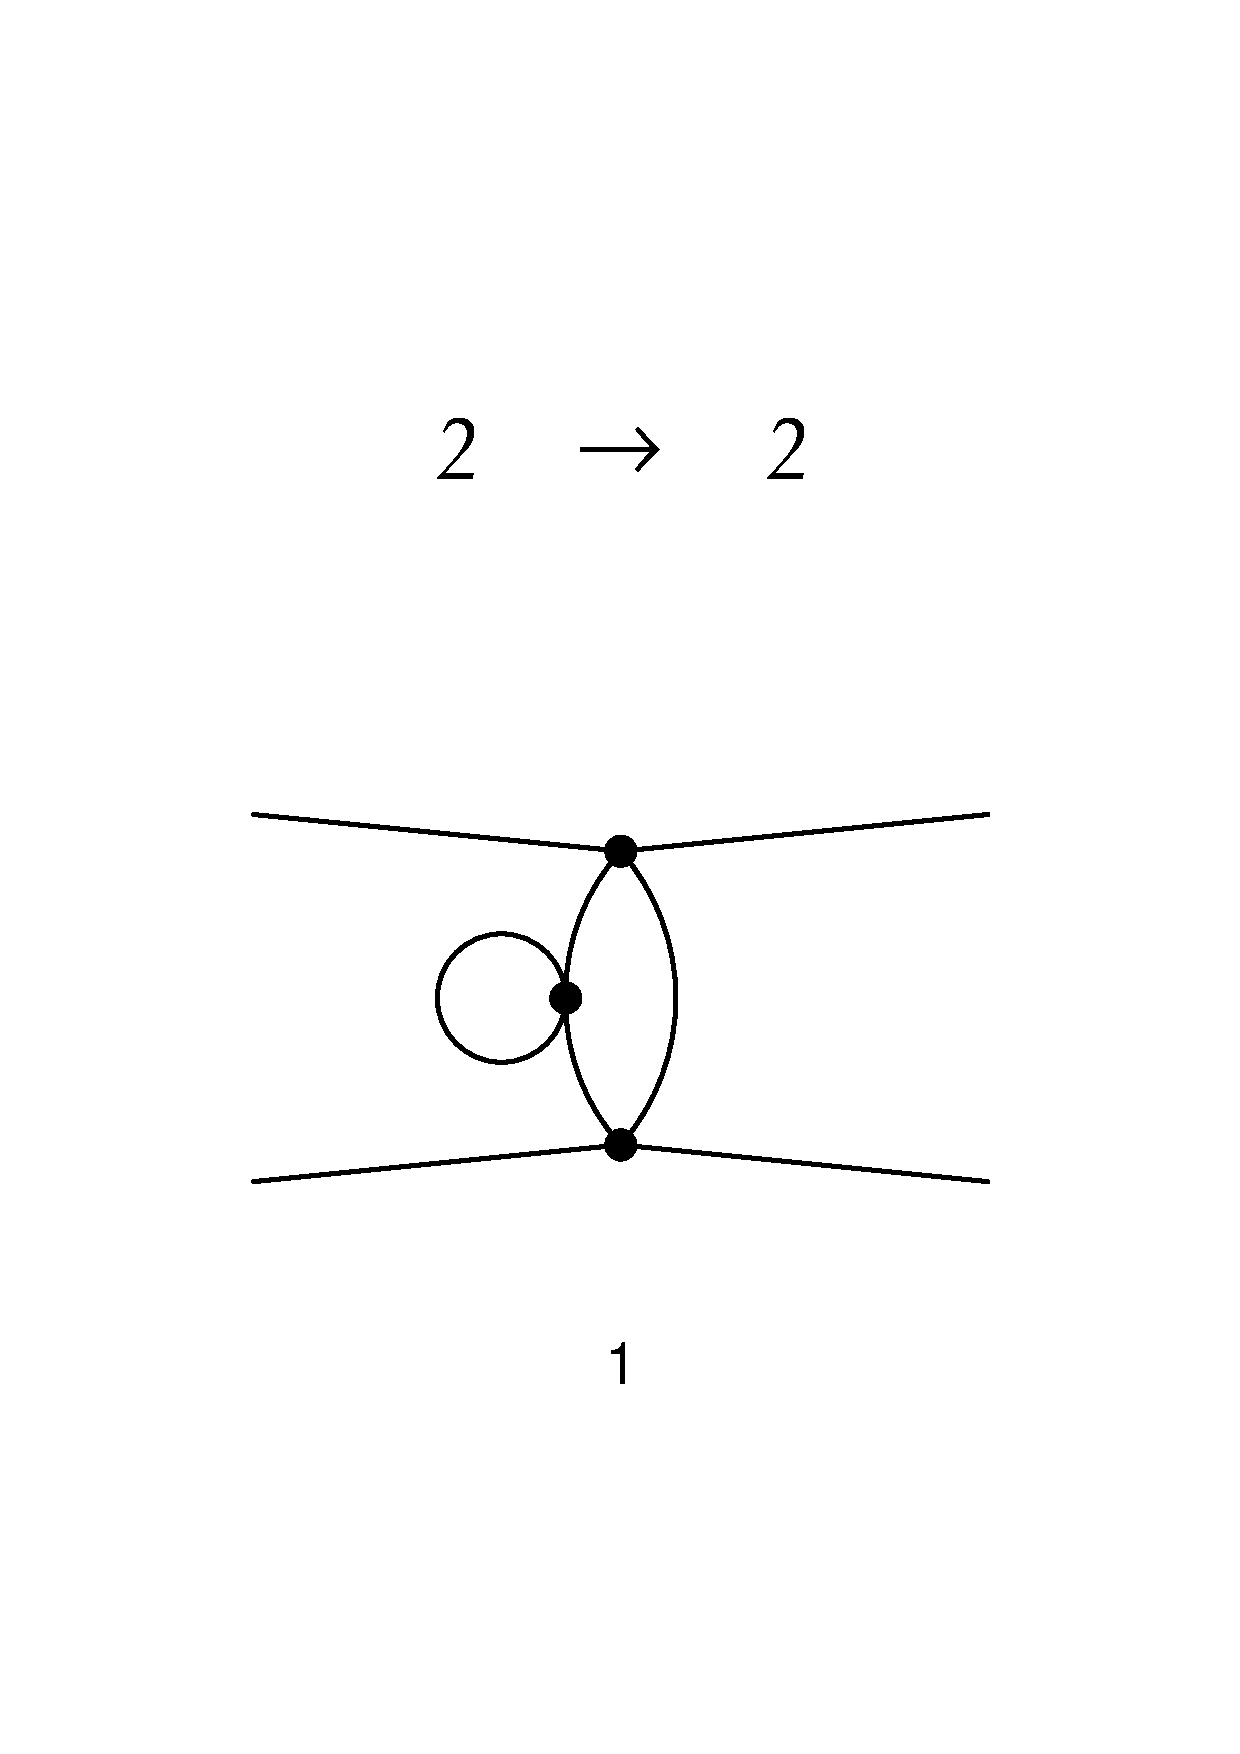
\includegraphics[width=0.28\textwidth]{generated/L2/images/topology8.pdf}
\end{center}
\noindent Parsed propagators: 8. Internal vertices: 3. Internal half-edges: 12.\\
\noindent Assignments checked: 32768. Surviving (nonzero vertex weight): 4096.\\
\noindent Raw $N_c$ power: 1. Net power in $C(t)$: -3.
\[\text{No surviving SK contributions for this topology.}\]
\section*{Topology 9 (FeynArts Topology 2)}
\begin{center}
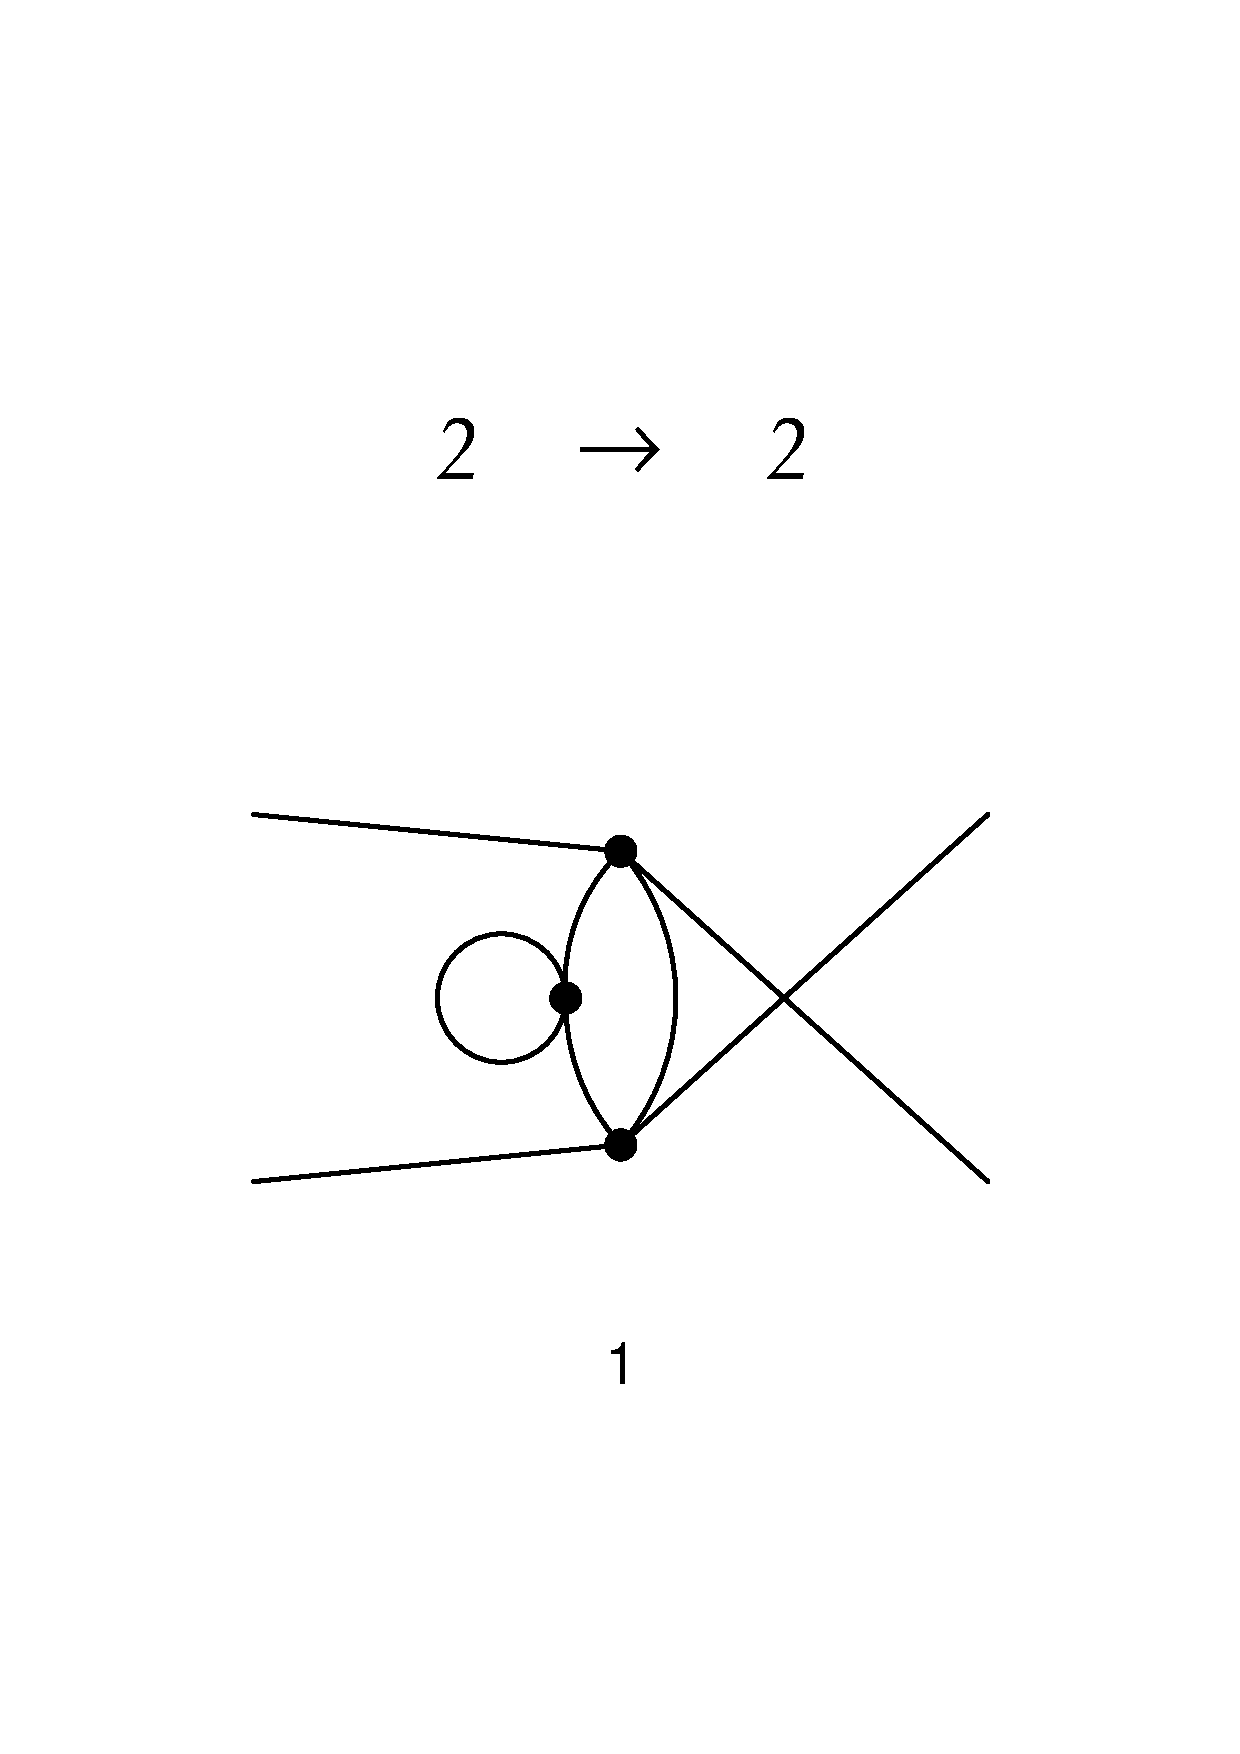
\includegraphics[width=0.28\textwidth]{generated/L2/images/topology9.pdf}
\end{center}
\noindent Parsed propagators: 8. Internal vertices: 3. Internal half-edges: 12.\\
\noindent Assignments checked: 32768. Surviving (nonzero vertex weight): 4096.\\
\noindent Raw $N_c$ power: 1. Net power in $C(t)$: -3.
\[\text{No surviving SK contributions for this topology.}\]
\section*{Topology 10 (FeynArts Topology 4)}
\begin{center}
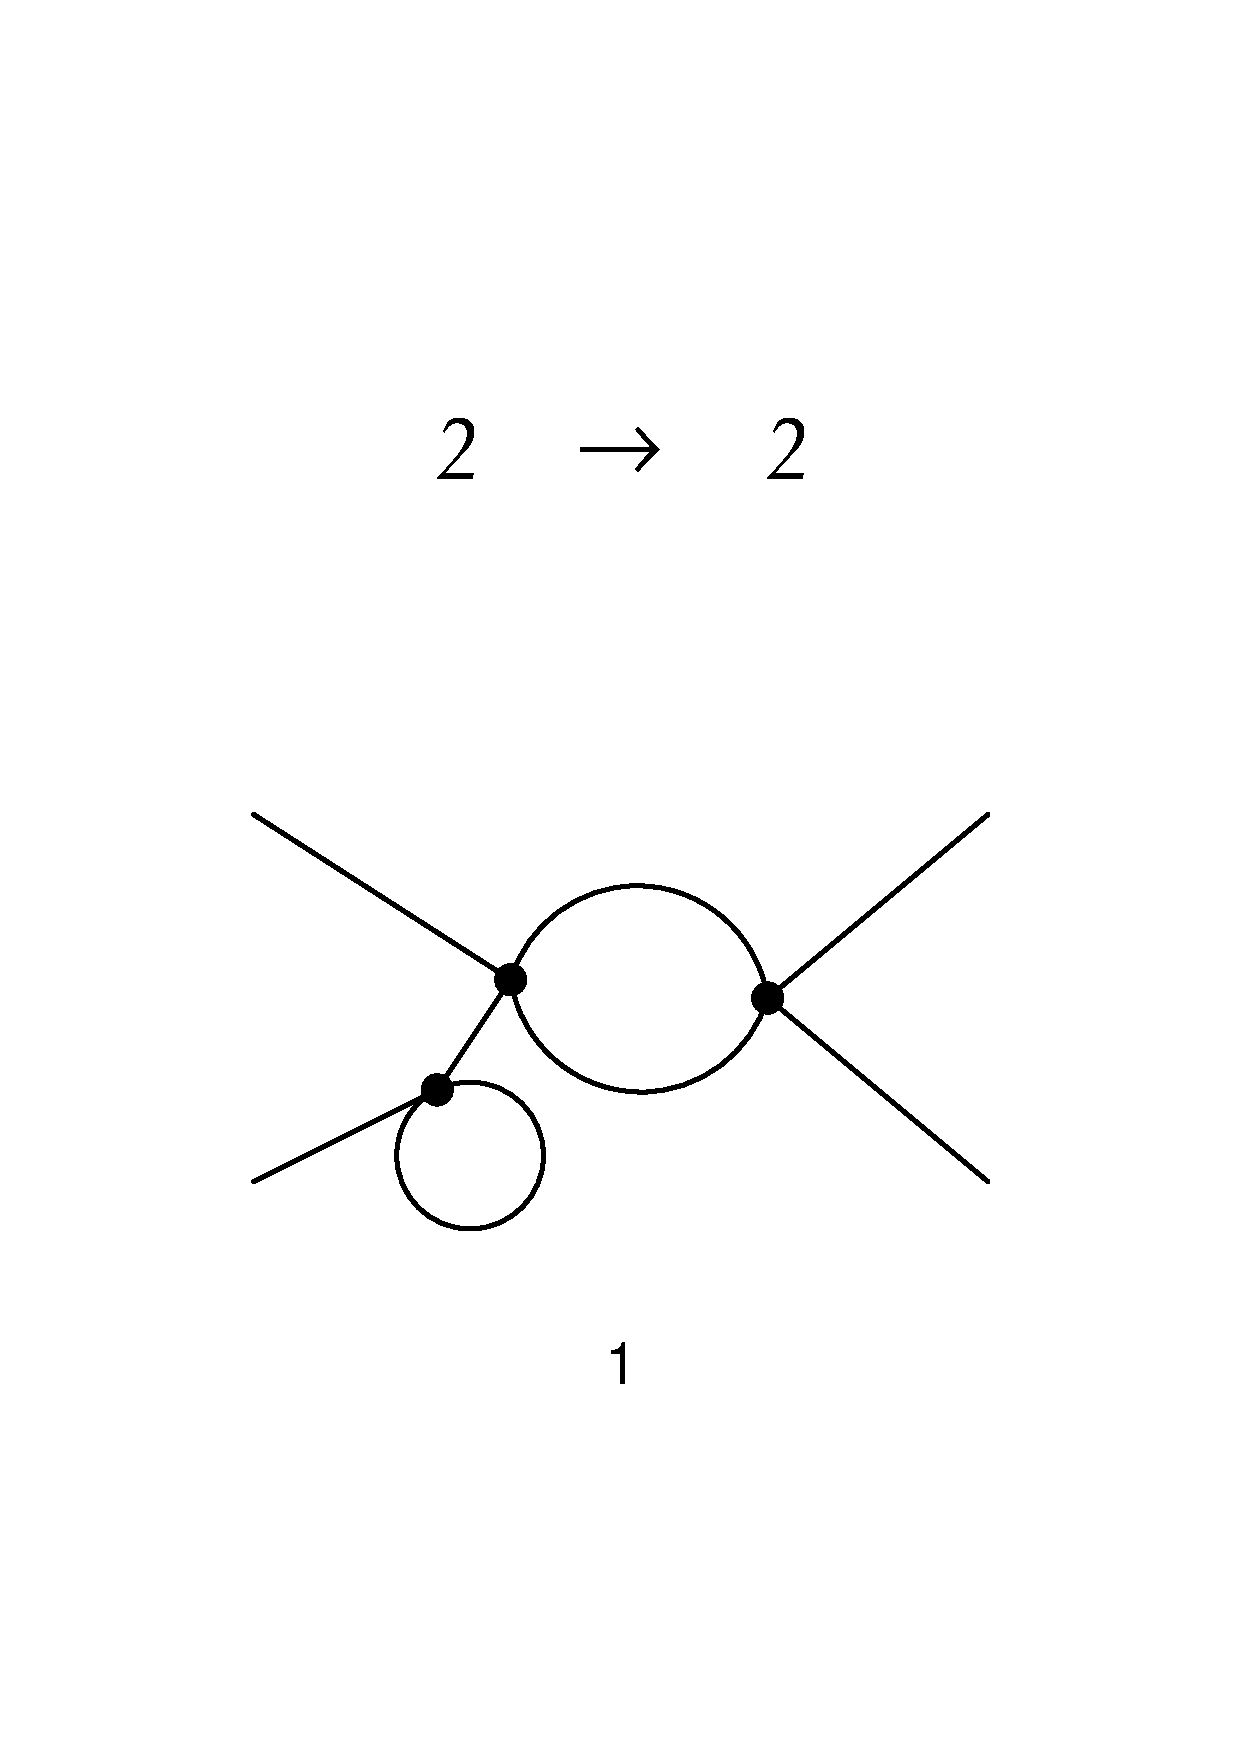
\includegraphics[width=0.28\textwidth]{generated/L2/images/topology10.pdf}
\end{center}
\noindent Parsed propagators: 8. Internal vertices: 3. Internal half-edges: 12.\\
\noindent Assignments checked: 32768. Surviving (nonzero vertex weight): 4096.\\
\noindent Raw $N_c$ power: 1. Net power in $C(t)$: -3.
\noindent Explicit surviving terms:
\begin{equation*}
\mathcal{T}_{10,1} = 128 i g_{2}^{3}\,N_c^{-3}\,G^<\left(x_1,z_{1}\right) \, G^<\left(z_{2},z_{1}\right) \, G_A\left(x_2,z_{2}\right) \, G_A\left(x_4,z_{3}\right) \, G_A\left(z_{1},z_{3}\right) \, G_A\left(z_{2},z_{2}\right) \, G_K\left(x_3,z_{3}\right) \, G_R\left(z_{1},z_{3}\right)
\end{equation*}
\begin{equation*}
\mathcal{T}_{10,2} = 128 i g_{2}^{3}\,N_c^{-3}\,G^<\left(x_1,z_{1}\right) \, G^<\left(z_{2},z_{1}\right) \, G_A\left(x_2,z_{2}\right) \, G_A\left(x_4,z_{3}\right) \, G_A\left(z_{1},z_{3}\right) \, G_A\left(z_{2},z_{2}\right) \, G_K\left(z_{1},z_{3}\right) \, G_R\left(x_3,z_{3}\right)
\end{equation*}
\begin{equation*}
\mathcal{T}_{10,3} = 128 i g_{2}^{3}\,N_c^{-3}\,G^<\left(x_1,z_{1}\right) \, G^<\left(z_{2},z_{1}\right) \, G_A\left(x_2,z_{2}\right) \, G_A\left(x_4,z_{3}\right) \, G_A\left(z_{1},z_{3}\right) \, G_K\left(x_3,z_{3}\right) \, G_R\left(z_{1},z_{3}\right) \, G_R\left(z_{2},z_{2}\right)
\end{equation*}
\begin{equation*}
\mathcal{T}_{10,4} = 128 i g_{2}^{3}\,N_c^{-3}\,G^<\left(x_1,z_{1}\right) \, G^<\left(z_{2},z_{1}\right) \, G_A\left(x_2,z_{2}\right) \, G_A\left(x_4,z_{3}\right) \, G_A\left(z_{1},z_{3}\right) \, G_K\left(z_{1},z_{3}\right) \, G_R\left(x_3,z_{3}\right) \, G_R\left(z_{2},z_{2}\right)
\end{equation*}
\begin{equation*}
\mathcal{T}_{10,5} = 64 i g_{2}^{3}\,N_c^{-3}\,G^<\left(z_{1},z_{3}\right) \, G^<\left(z_{1},z_{3}\right) \, G_A\left(x_2,z_{2}\right) \, G_A\left(x_4,z_{3}\right) \, G_A\left(z_{2},z_{1}\right) \, G_K\left(z_{2},z_{2}\right) \, G_R\left(x_1,z_{1}\right) \, G_R\left(x_3,z_{3}\right)
\end{equation*}
\begin{equation*}
\mathcal{T}_{10,6} = 64 i g_{2}^{3}\,N_c^{-3}\,G^<\left(z_{1},z_{3}\right) \, G^<\left(z_{1},z_{3}\right) \, G_A\left(x_2,z_{2}\right) \, G_A\left(x_4,z_{3}\right) \, G_A\left(z_{2},z_{2}\right) \, G_K\left(x_1,z_{1}\right) \, G_R\left(x_3,z_{3}\right) \, G_R\left(z_{2},z_{1}\right)
\end{equation*}
\begin{equation*}
\mathcal{T}_{10,7} = 64 i g_{2}^{3}\,N_c^{-3}\,G^<\left(z_{1},z_{3}\right) \, G^<\left(z_{1},z_{3}\right) \, G_A\left(x_2,z_{2}\right) \, G_A\left(x_4,z_{3}\right) \, G_A\left(z_{2},z_{2}\right) \, G_K\left(z_{2},z_{1}\right) \, G_R\left(x_1,z_{1}\right) \, G_R\left(x_3,z_{3}\right)
\end{equation*}
\begin{equation*}
\mathcal{T}_{10,8} = 64 i g_{2}^{3}\,N_c^{-3}\,G^<\left(z_{1},z_{3}\right) \, G^<\left(z_{1},z_{3}\right) \, G_A\left(x_2,z_{2}\right) \, G_A\left(x_4,z_{3}\right) \, G_K\left(x_1,z_{1}\right) \, G_R\left(x_3,z_{3}\right) \, G_R\left(z_{2},z_{1}\right) \, G_R\left(z_{2},z_{2}\right)
\end{equation*}
\begin{equation*}
\mathcal{T}_{10,9} = 64 i g_{2}^{3}\,N_c^{-3}\,G^<\left(z_{1},z_{3}\right) \, G^<\left(z_{1},z_{3}\right) \, G_A\left(x_2,z_{2}\right) \, G_A\left(x_4,z_{3}\right) \, G_K\left(z_{2},z_{1}\right) \, G_R\left(x_1,z_{1}\right) \, G_R\left(x_3,z_{3}\right) \, G_R\left(z_{2},z_{2}\right)
\end{equation*}
\section*{Topology 11 (FeynArts Topology 4)}
\begin{center}
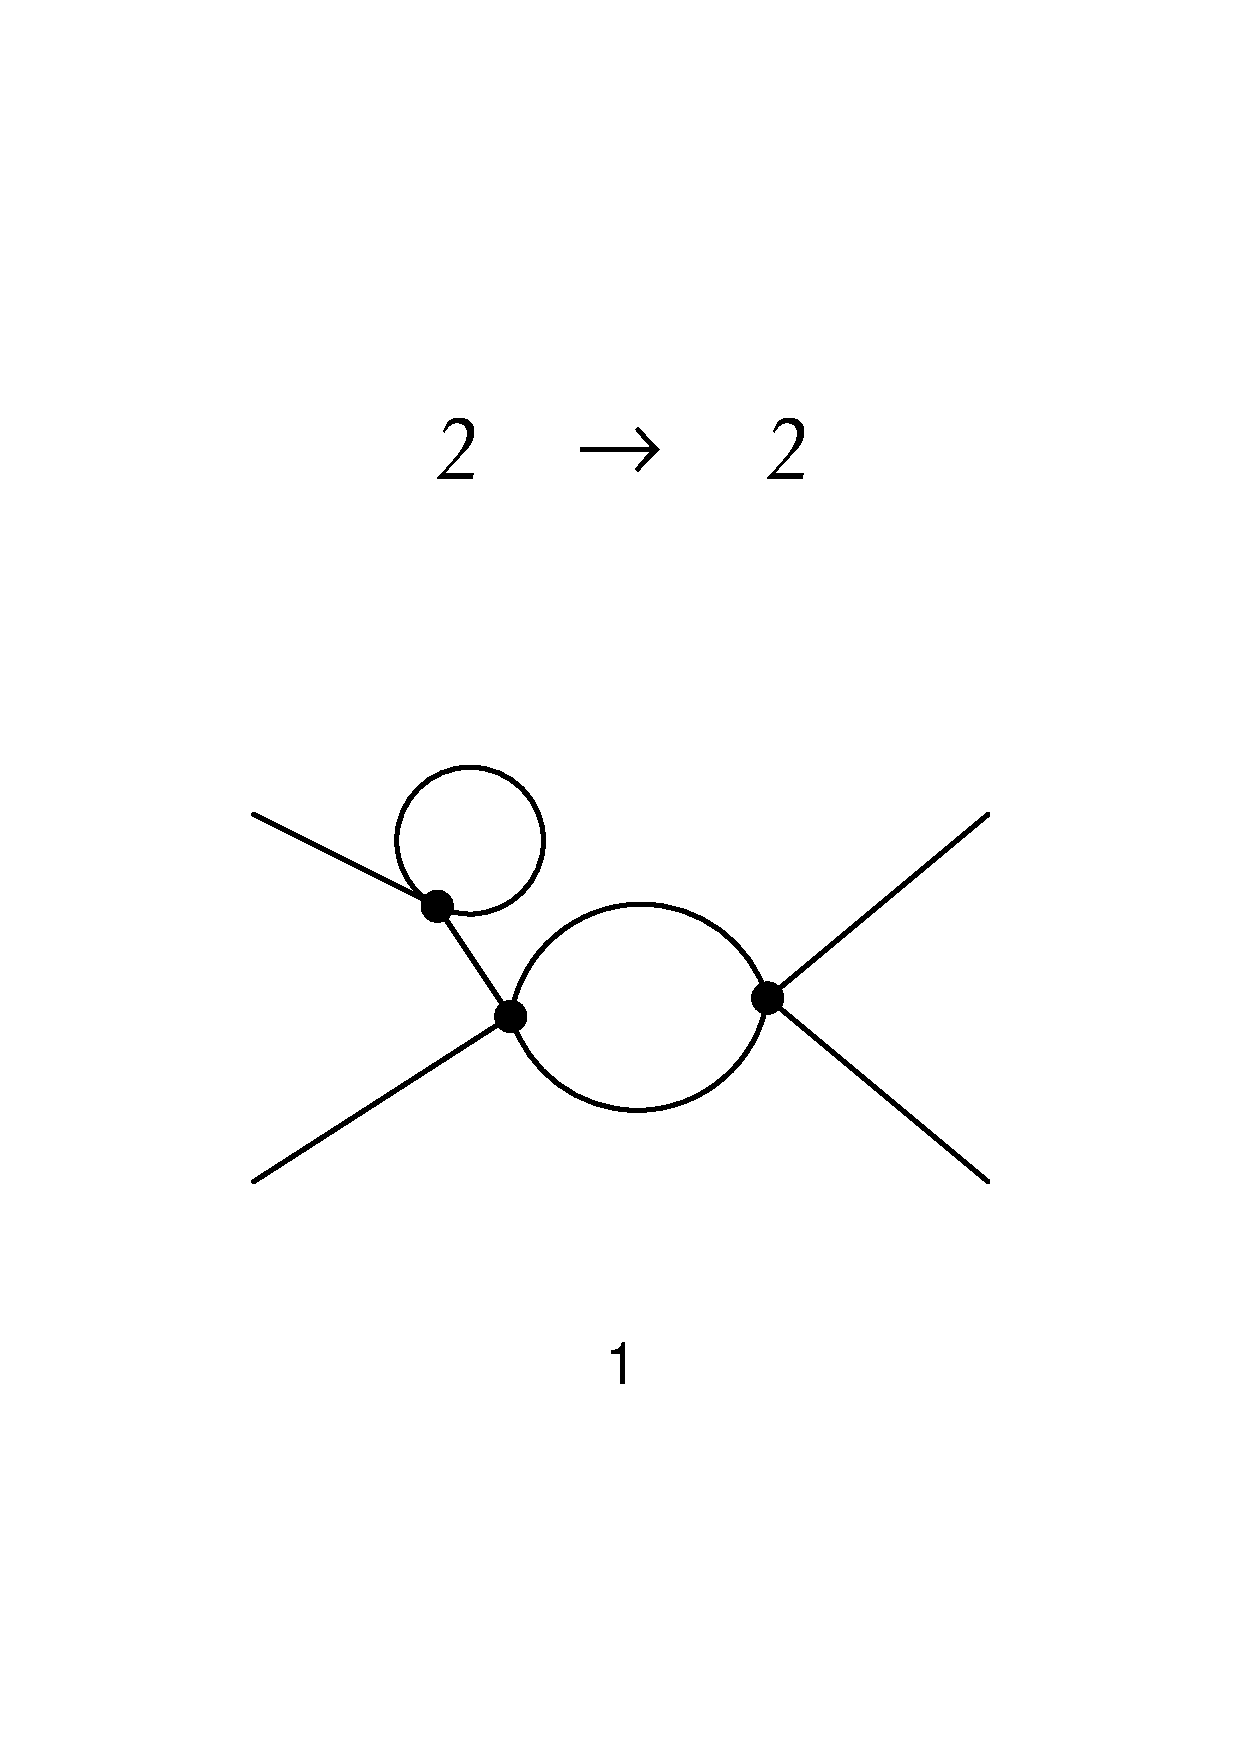
\includegraphics[width=0.28\textwidth]{generated/L2/images/topology11.pdf}
\end{center}
\noindent Parsed propagators: 8. Internal vertices: 3. Internal half-edges: 12.\\
\noindent Assignments checked: 32768. Surviving (nonzero vertex weight): 4096.\\
\noindent Raw $N_c$ power: 1. Net power in $C(t)$: -3.
\noindent Explicit surviving terms:
\begin{equation*}
\mathcal{T}_{11,1} = 64 i g_{2}^{3}\,N_c^{-3}\,G^<\left(z_{2},z_{3}\right) \, G^<\left(z_{2},z_{3}\right) \, G_A\left(x_2,z_{2}\right) \, G_A\left(x_4,z_{3}\right) \, G_A\left(z_{1},z_{1}\right) \, G_A\left(z_{2},z_{1}\right) \, G_K\left(x_1,z_{1}\right) \, G_R\left(x_3,z_{3}\right)
\end{equation*}
\begin{equation*}
\mathcal{T}_{11,2} = 64 i g_{2}^{3}\,N_c^{-3}\,G^<\left(z_{2},z_{3}\right) \, G^<\left(z_{2},z_{3}\right) \, G_A\left(x_2,z_{2}\right) \, G_A\left(x_4,z_{3}\right) \, G_A\left(z_{2},z_{1}\right) \, G_K\left(x_1,z_{1}\right) \, G_R\left(x_3,z_{3}\right) \, G_R\left(z_{1},z_{1}\right)
\end{equation*}
\begin{equation*}
\mathcal{T}_{11,3} = 64 i g_{2}^{3}\,N_c^{-3}\,G^<\left(z_{2},z_{3}\right) \, G^<\left(z_{2},z_{3}\right) \, G_A\left(x_2,z_{2}\right) \, G_A\left(x_4,z_{3}\right) \, G_A\left(z_{2},z_{1}\right) \, G_K\left(z_{1},z_{1}\right) \, G_R\left(x_1,z_{1}\right) \, G_R\left(x_3,z_{3}\right)
\end{equation*}
\section*{Topology 12 (FeynArts Topology 4)}
\begin{center}
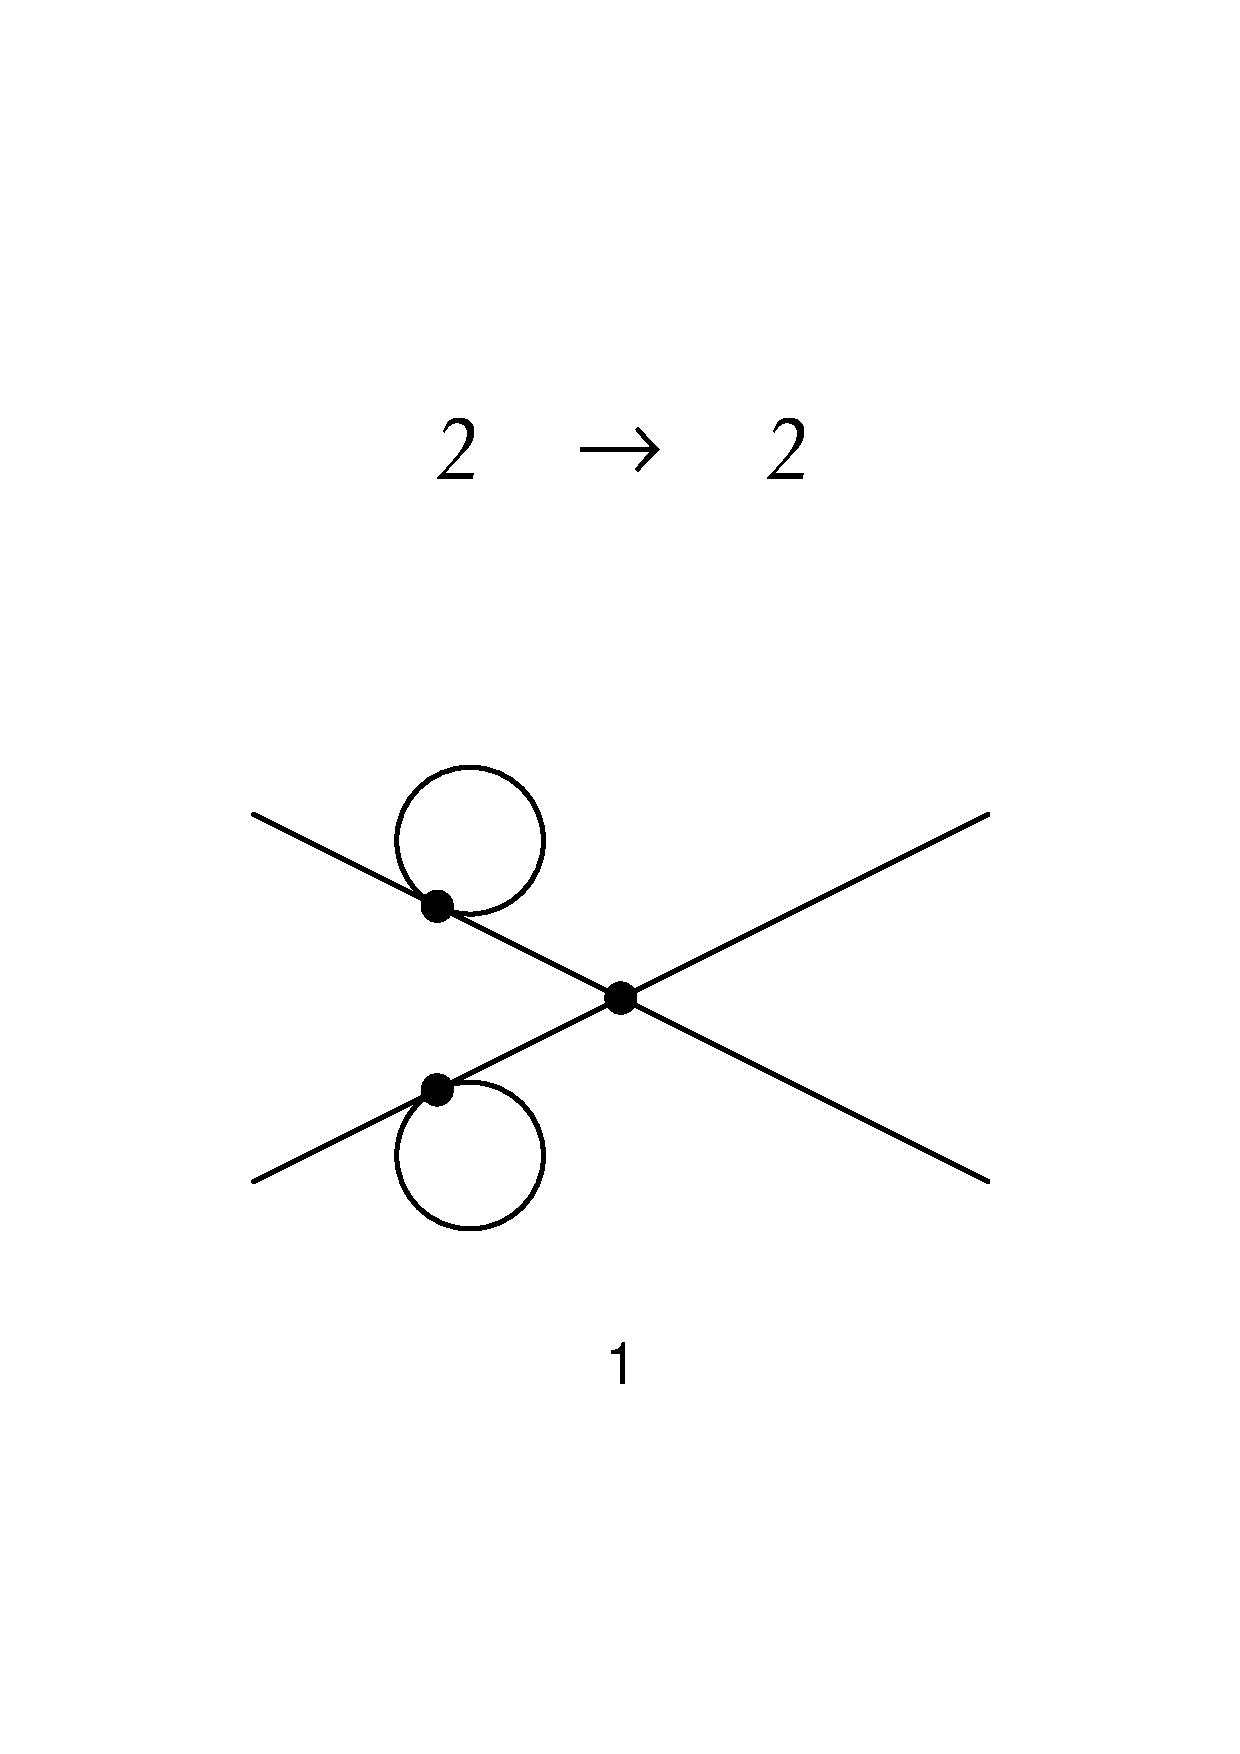
\includegraphics[width=0.28\textwidth]{generated/L2/images/topology12.pdf}
\end{center}
\noindent Parsed propagators: 8. Internal vertices: 3. Internal half-edges: 12.\\
\noindent Assignments checked: 32768. Surviving (nonzero vertex weight): 4096.\\
\noindent Raw $N_c$ power: 2. Net power in $C(t)$: -2.
\noindent Explicit surviving terms:
\begin{equation*}
\mathcal{T}_{12,1} = 64 i g_{2}^{3}\,N_c^{-2}\,G^<\left(x_1,z_{1}\right) \, G^<\left(z_{2},z_{3}\right) \, G_A\left(x_2,z_{2}\right) \, G_A\left(x_4,z_{3}\right) \, G_A\left(z_{1},z_{1}\right) \, G_A\left(z_{2},z_{2}\right) \, G_K\left(x_3,z_{3}\right) \, G_R\left(z_{1},z_{3}\right)
\end{equation*}
\begin{equation*}
\mathcal{T}_{12,2} = 64 i g_{2}^{3}\,N_c^{-2}\,G^<\left(x_1,z_{1}\right) \, G^<\left(z_{2},z_{3}\right) \, G_A\left(x_2,z_{2}\right) \, G_A\left(x_4,z_{3}\right) \, G_A\left(z_{1},z_{1}\right) \, G_A\left(z_{2},z_{2}\right) \, G_K\left(z_{1},z_{3}\right) \, G_R\left(x_3,z_{3}\right)
\end{equation*}
\begin{equation*}
\mathcal{T}_{12,3} = 64 i g_{2}^{3}\,N_c^{-2}\,G^<\left(x_1,z_{1}\right) \, G^<\left(z_{2},z_{3}\right) \, G_A\left(x_2,z_{2}\right) \, G_A\left(x_4,z_{3}\right) \, G_A\left(z_{1},z_{1}\right) \, G_K\left(x_3,z_{3}\right) \, G_R\left(z_{1},z_{3}\right) \, G_R\left(z_{2},z_{2}\right)
\end{equation*}
\begin{equation*}
\mathcal{T}_{12,4} = 64 i g_{2}^{3}\,N_c^{-2}\,G^<\left(x_1,z_{1}\right) \, G^<\left(z_{2},z_{3}\right) \, G_A\left(x_2,z_{2}\right) \, G_A\left(x_4,z_{3}\right) \, G_A\left(z_{1},z_{1}\right) \, G_K\left(z_{1},z_{3}\right) \, G_R\left(x_3,z_{3}\right) \, G_R\left(z_{2},z_{2}\right)
\end{equation*}
\begin{equation*}
\mathcal{T}_{12,5} = 64 i g_{2}^{3}\,N_c^{-2}\,G^<\left(x_1,z_{1}\right) \, G^<\left(z_{2},z_{3}\right) \, G_A\left(x_2,z_{2}\right) \, G_A\left(x_4,z_{3}\right) \, G_A\left(z_{1},z_{3}\right) \, G_A\left(z_{2},z_{2}\right) \, G_K\left(z_{1},z_{1}\right) \, G_R\left(x_3,z_{3}\right)
\end{equation*}
\begin{equation*}
\mathcal{T}_{12,6} = 64 i g_{2}^{3}\,N_c^{-2}\,G^<\left(x_1,z_{1}\right) \, G^<\left(z_{2},z_{3}\right) \, G_A\left(x_2,z_{2}\right) \, G_A\left(x_4,z_{3}\right) \, G_A\left(z_{1},z_{3}\right) \, G_K\left(z_{1},z_{1}\right) \, G_R\left(x_3,z_{3}\right) \, G_R\left(z_{2},z_{2}\right)
\end{equation*}
\begin{equation*}
\mathcal{T}_{12,7} = 64 i g_{2}^{3}\,N_c^{-2}\,G^<\left(x_1,z_{1}\right) \, G^<\left(z_{2},z_{3}\right) \, G_A\left(x_2,z_{2}\right) \, G_A\left(x_4,z_{3}\right) \, G_A\left(z_{2},z_{2}\right) \, G_K\left(x_3,z_{3}\right) \, G_R\left(z_{1},z_{1}\right) \, G_R\left(z_{1},z_{3}\right)
\end{equation*}
\begin{equation*}
\mathcal{T}_{12,8} = 64 i g_{2}^{3}\,N_c^{-2}\,G^<\left(x_1,z_{1}\right) \, G^<\left(z_{2},z_{3}\right) \, G_A\left(x_2,z_{2}\right) \, G_A\left(x_4,z_{3}\right) \, G_A\left(z_{2},z_{2}\right) \, G_K\left(z_{1},z_{3}\right) \, G_R\left(x_3,z_{3}\right) \, G_R\left(z_{1},z_{1}\right)
\end{equation*}
\begin{equation*}
\mathcal{T}_{12,9} = 64 i g_{2}^{3}\,N_c^{-2}\,G^<\left(x_1,z_{1}\right) \, G^<\left(z_{2},z_{3}\right) \, G_A\left(x_2,z_{2}\right) \, G_A\left(x_4,z_{3}\right) \, G_K\left(x_3,z_{3}\right) \, G_R\left(z_{1},z_{1}\right) \, G_R\left(z_{1},z_{3}\right) \, G_R\left(z_{2},z_{2}\right)
\end{equation*}
\begin{equation*}
\mathcal{T}_{12,10} = 64 i g_{2}^{3}\,N_c^{-2}\,G^<\left(x_1,z_{1}\right) \, G^<\left(z_{2},z_{3}\right) \, G_A\left(x_2,z_{2}\right) \, G_A\left(x_4,z_{3}\right) \, G_K\left(z_{1},z_{3}\right) \, G_R\left(x_3,z_{3}\right) \, G_R\left(z_{1},z_{1}\right) \, G_R\left(z_{2},z_{2}\right)
\end{equation*}
\begin{equation*}
\mathcal{T}_{12,11} = 64 i g_{2}^{3}\,N_c^{-2}\,G^<\left(z_{1},z_{3}\right) \, G^<\left(z_{2},z_{3}\right) \, G_A\left(x_2,z_{2}\right) \, G_A\left(x_4,z_{3}\right) \, G_A\left(z_{1},z_{1}\right) \, G_A\left(z_{2},z_{2}\right) \, G_K\left(x_1,z_{1}\right) \, G_R\left(x_3,z_{3}\right)
\end{equation*}
\begin{equation*}
\mathcal{T}_{12,12} = 64 i g_{2}^{3}\,N_c^{-2}\,G^<\left(z_{1},z_{3}\right) \, G^<\left(z_{2},z_{3}\right) \, G_A\left(x_2,z_{2}\right) \, G_A\left(x_4,z_{3}\right) \, G_A\left(z_{1},z_{1}\right) \, G_K\left(x_1,z_{1}\right) \, G_R\left(x_3,z_{3}\right) \, G_R\left(z_{2},z_{2}\right)
\end{equation*}
\begin{equation*}
\mathcal{T}_{12,13} = 64 i g_{2}^{3}\,N_c^{-2}\,G^<\left(z_{1},z_{3}\right) \, G^<\left(z_{2},z_{3}\right) \, G_A\left(x_2,z_{2}\right) \, G_A\left(x_4,z_{3}\right) \, G_A\left(z_{2},z_{2}\right) \, G_K\left(x_1,z_{1}\right) \, G_R\left(x_3,z_{3}\right) \, G_R\left(z_{1},z_{1}\right)
\end{equation*}
\begin{equation*}
\mathcal{T}_{12,14} = 64 i g_{2}^{3}\,N_c^{-2}\,G^<\left(z_{1},z_{3}\right) \, G^<\left(z_{2},z_{3}\right) \, G_A\left(x_2,z_{2}\right) \, G_A\left(x_4,z_{3}\right) \, G_A\left(z_{2},z_{2}\right) \, G_K\left(z_{1},z_{1}\right) \, G_R\left(x_1,z_{1}\right) \, G_R\left(x_3,z_{3}\right)
\end{equation*}
\begin{equation*}
\mathcal{T}_{12,15} = 64 i g_{2}^{3}\,N_c^{-2}\,G^<\left(z_{1},z_{3}\right) \, G^<\left(z_{2},z_{3}\right) \, G_A\left(x_2,z_{2}\right) \, G_A\left(x_4,z_{3}\right) \, G_K\left(x_1,z_{1}\right) \, G_R\left(x_3,z_{3}\right) \, G_R\left(z_{1},z_{1}\right) \, G_R\left(z_{2},z_{2}\right)
\end{equation*}
\begin{equation*}
\mathcal{T}_{12,16} = 64 i g_{2}^{3}\,N_c^{-2}\,G^<\left(z_{1},z_{3}\right) \, G^<\left(z_{2},z_{3}\right) \, G_A\left(x_2,z_{2}\right) \, G_A\left(x_4,z_{3}\right) \, G_K\left(z_{1},z_{1}\right) \, G_R\left(x_1,z_{1}\right) \, G_R\left(x_3,z_{3}\right) \, G_R\left(z_{2},z_{2}\right)
\end{equation*}
\section*{Topology 13 (FeynArts Topology 4)}
\begin{center}
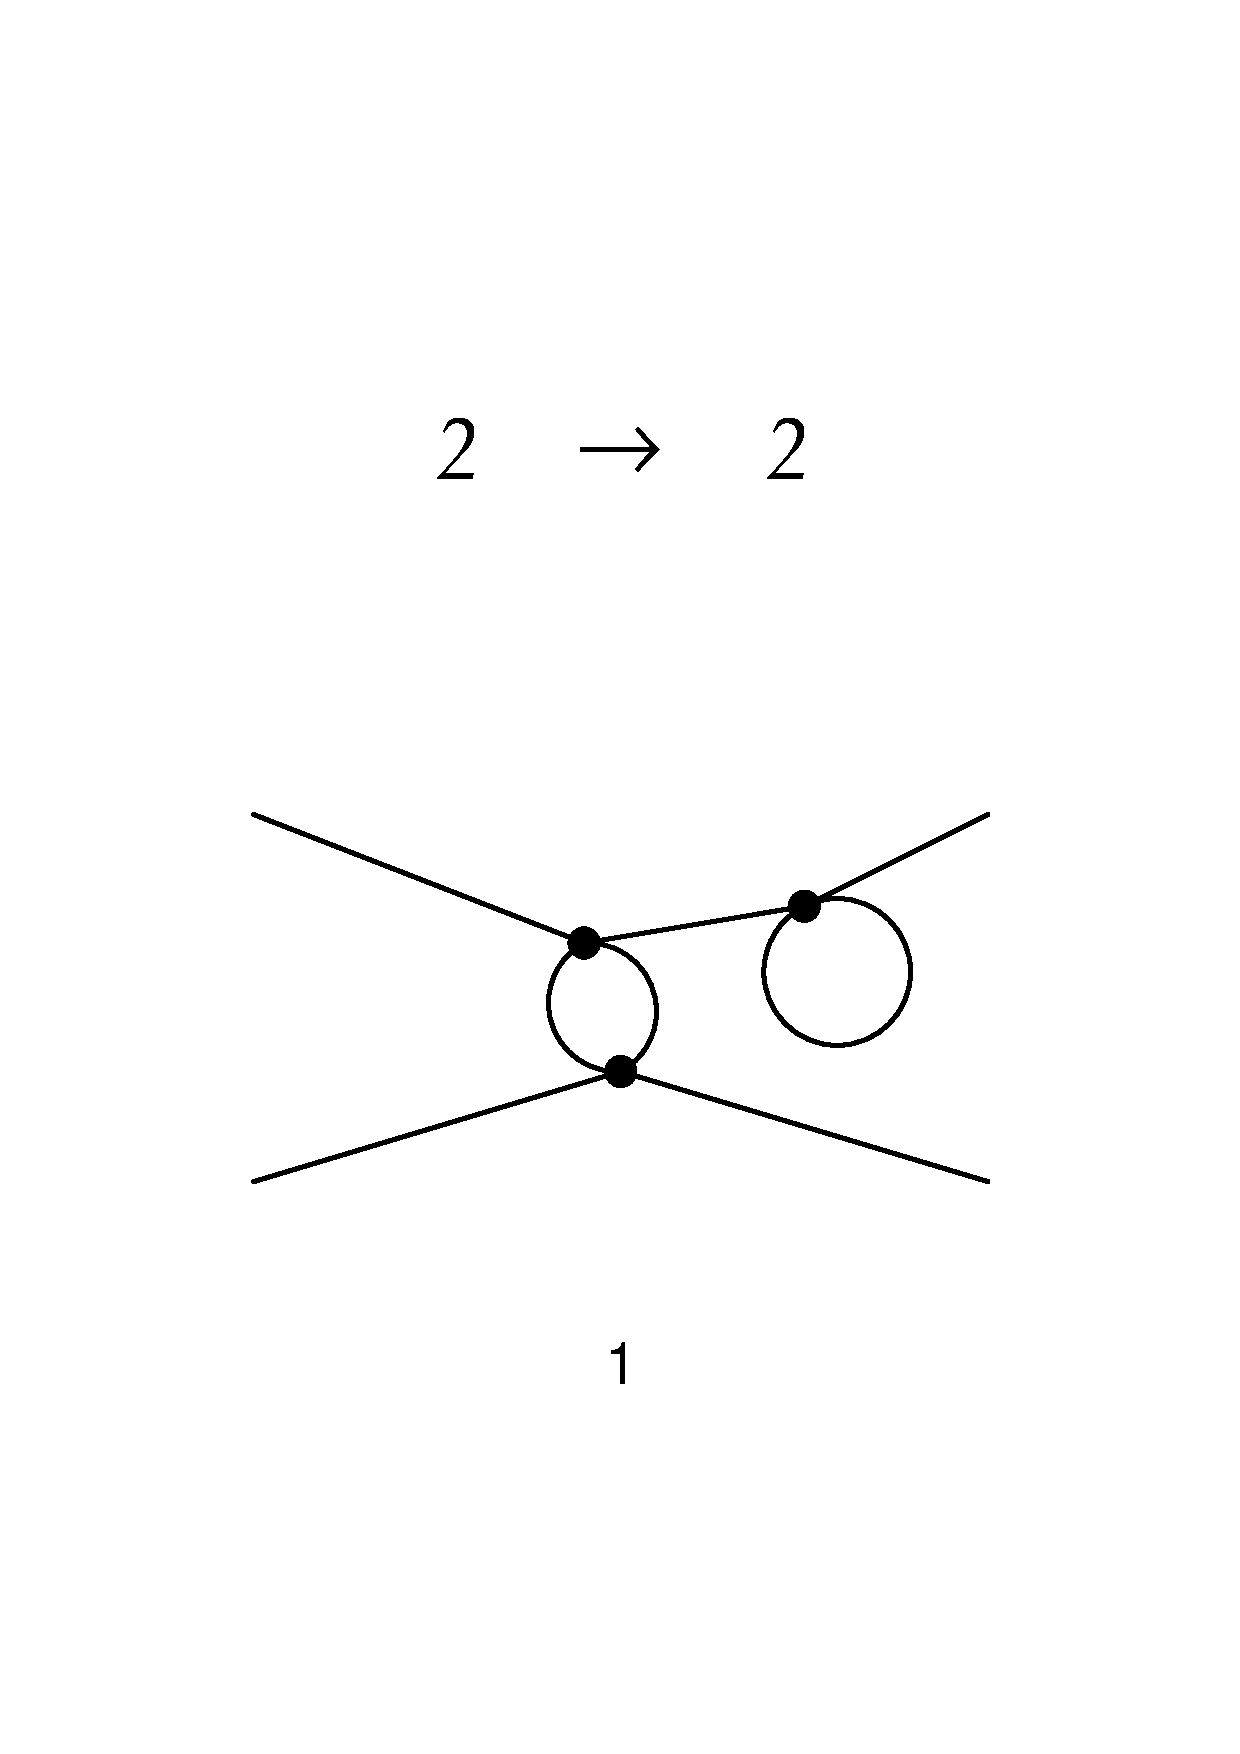
\includegraphics[width=0.28\textwidth]{generated/L2/images/topology13.pdf}
\end{center}
\noindent Parsed propagators: 8. Internal vertices: 3. Internal half-edges: 12.\\
\noindent Assignments checked: 32768. Surviving (nonzero vertex weight): 4096.\\
\noindent Raw $N_c$ power: 1. Net power in $C(t)$: -3.
\[\text{No surviving SK contributions for this topology.}\]
\section*{Topology 14 (FeynArts Topology 4)}
\begin{center}
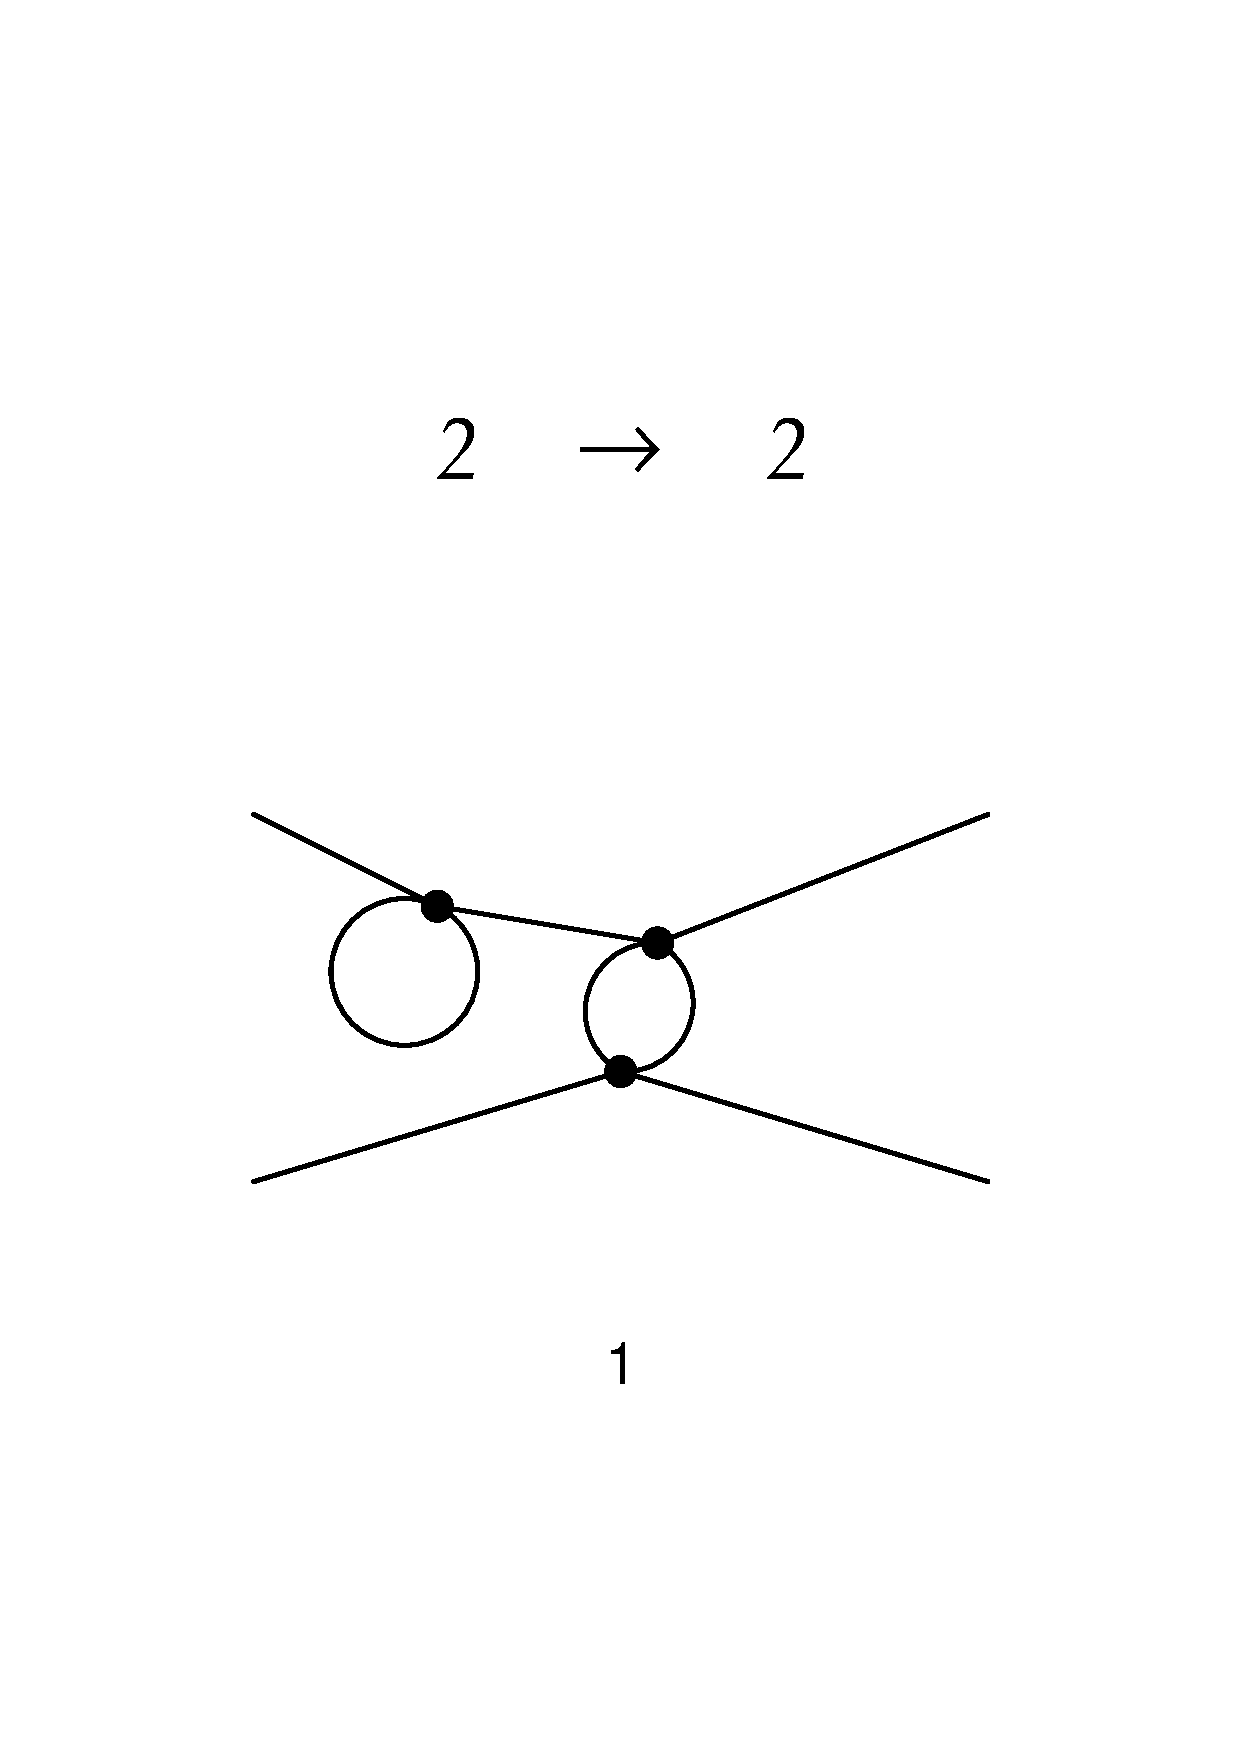
\includegraphics[width=0.28\textwidth]{generated/L2/images/topology14.pdf}
\end{center}
\noindent Parsed propagators: 8. Internal vertices: 3. Internal half-edges: 12.\\
\noindent Assignments checked: 32768. Surviving (nonzero vertex weight): 4096.\\
\noindent Raw $N_c$ power: 1. Net power in $C(t)$: -3.
\[\text{No surviving SK contributions for this topology.}\]
\section*{Topology 15 (FeynArts Topology 4)}
\begin{center}
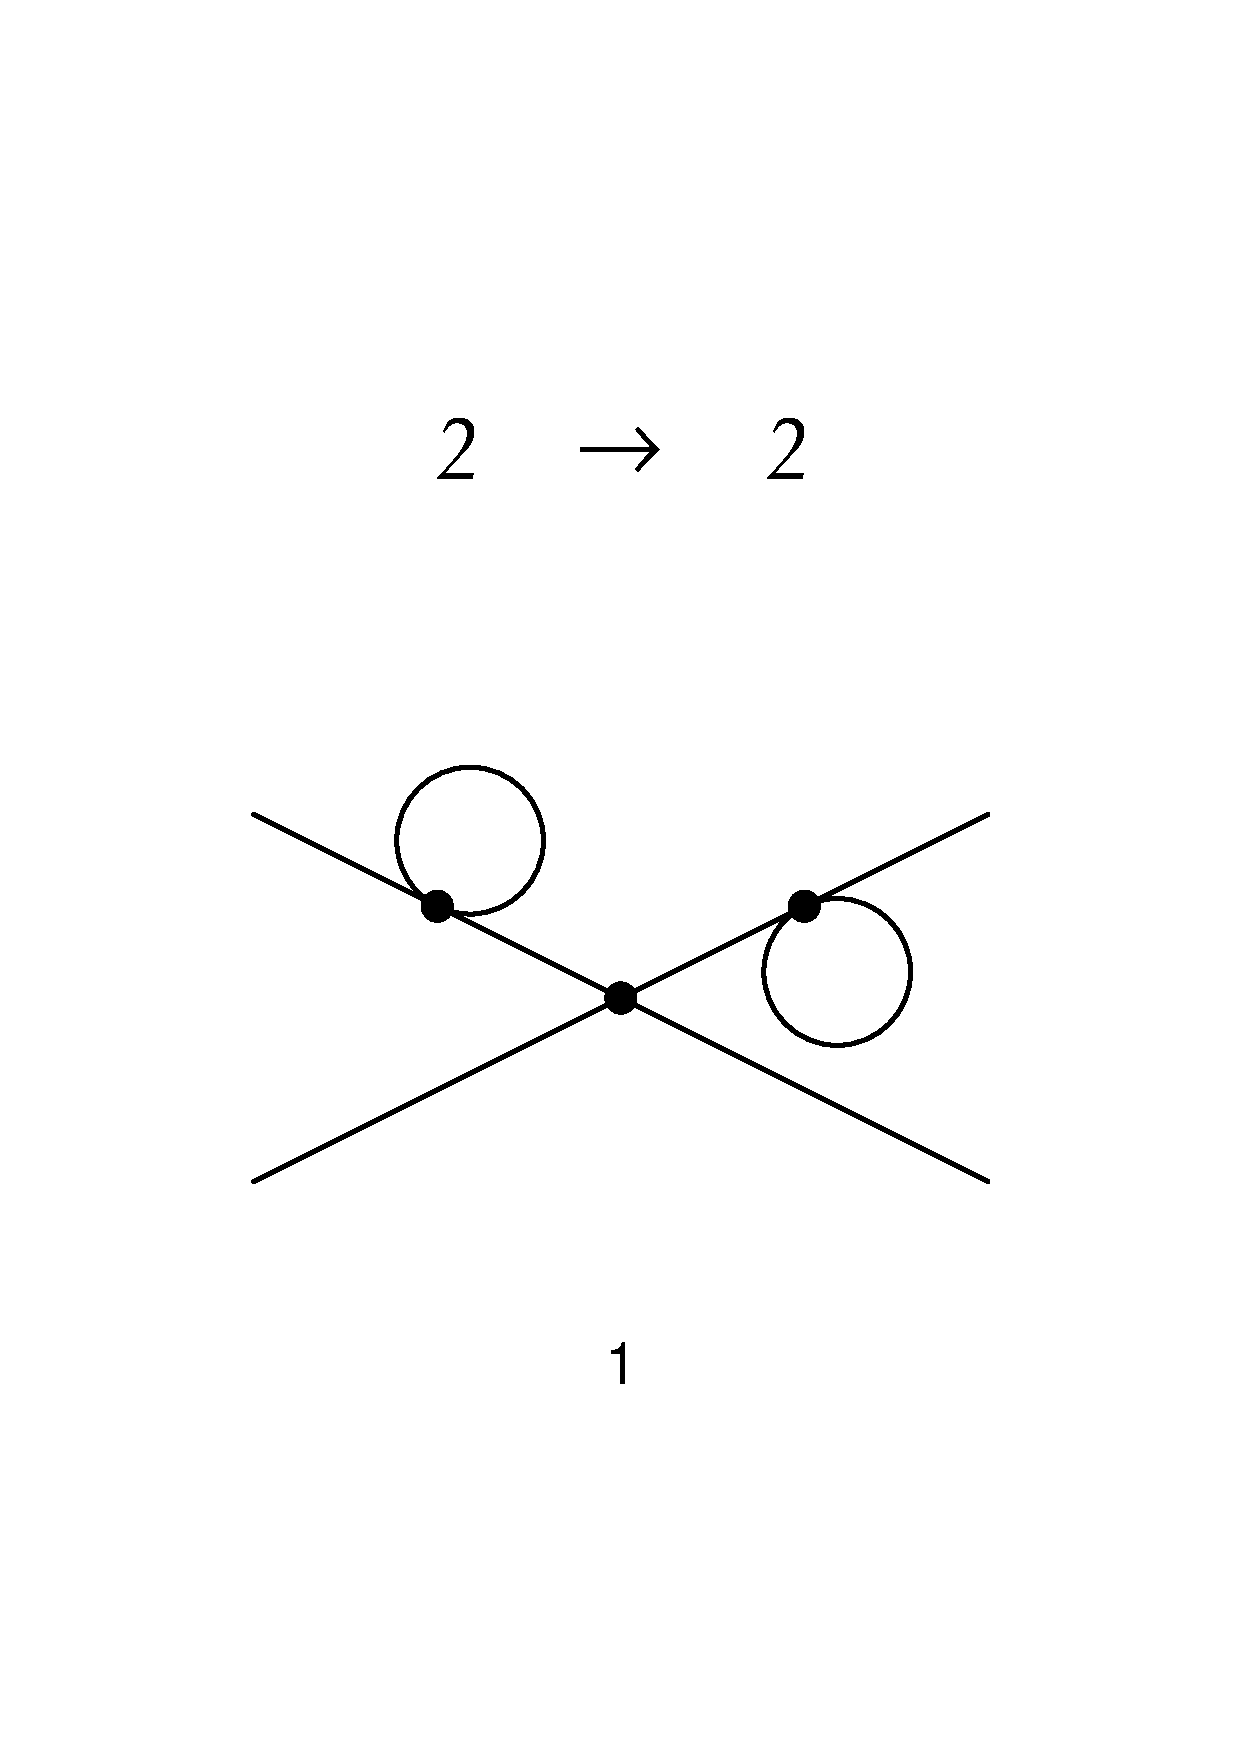
\includegraphics[width=0.28\textwidth]{generated/L2/images/topology15.pdf}
\end{center}
\noindent Parsed propagators: 8. Internal vertices: 3. Internal half-edges: 12.\\
\noindent Assignments checked: 32768. Surviving (nonzero vertex weight): 4096.\\
\noindent Raw $N_c$ power: 2. Net power in $C(t)$: -2.
\[\text{No surviving SK contributions for this topology.}\]
\section*{Topology 16 (FeynArts Topology 4)}
\begin{center}
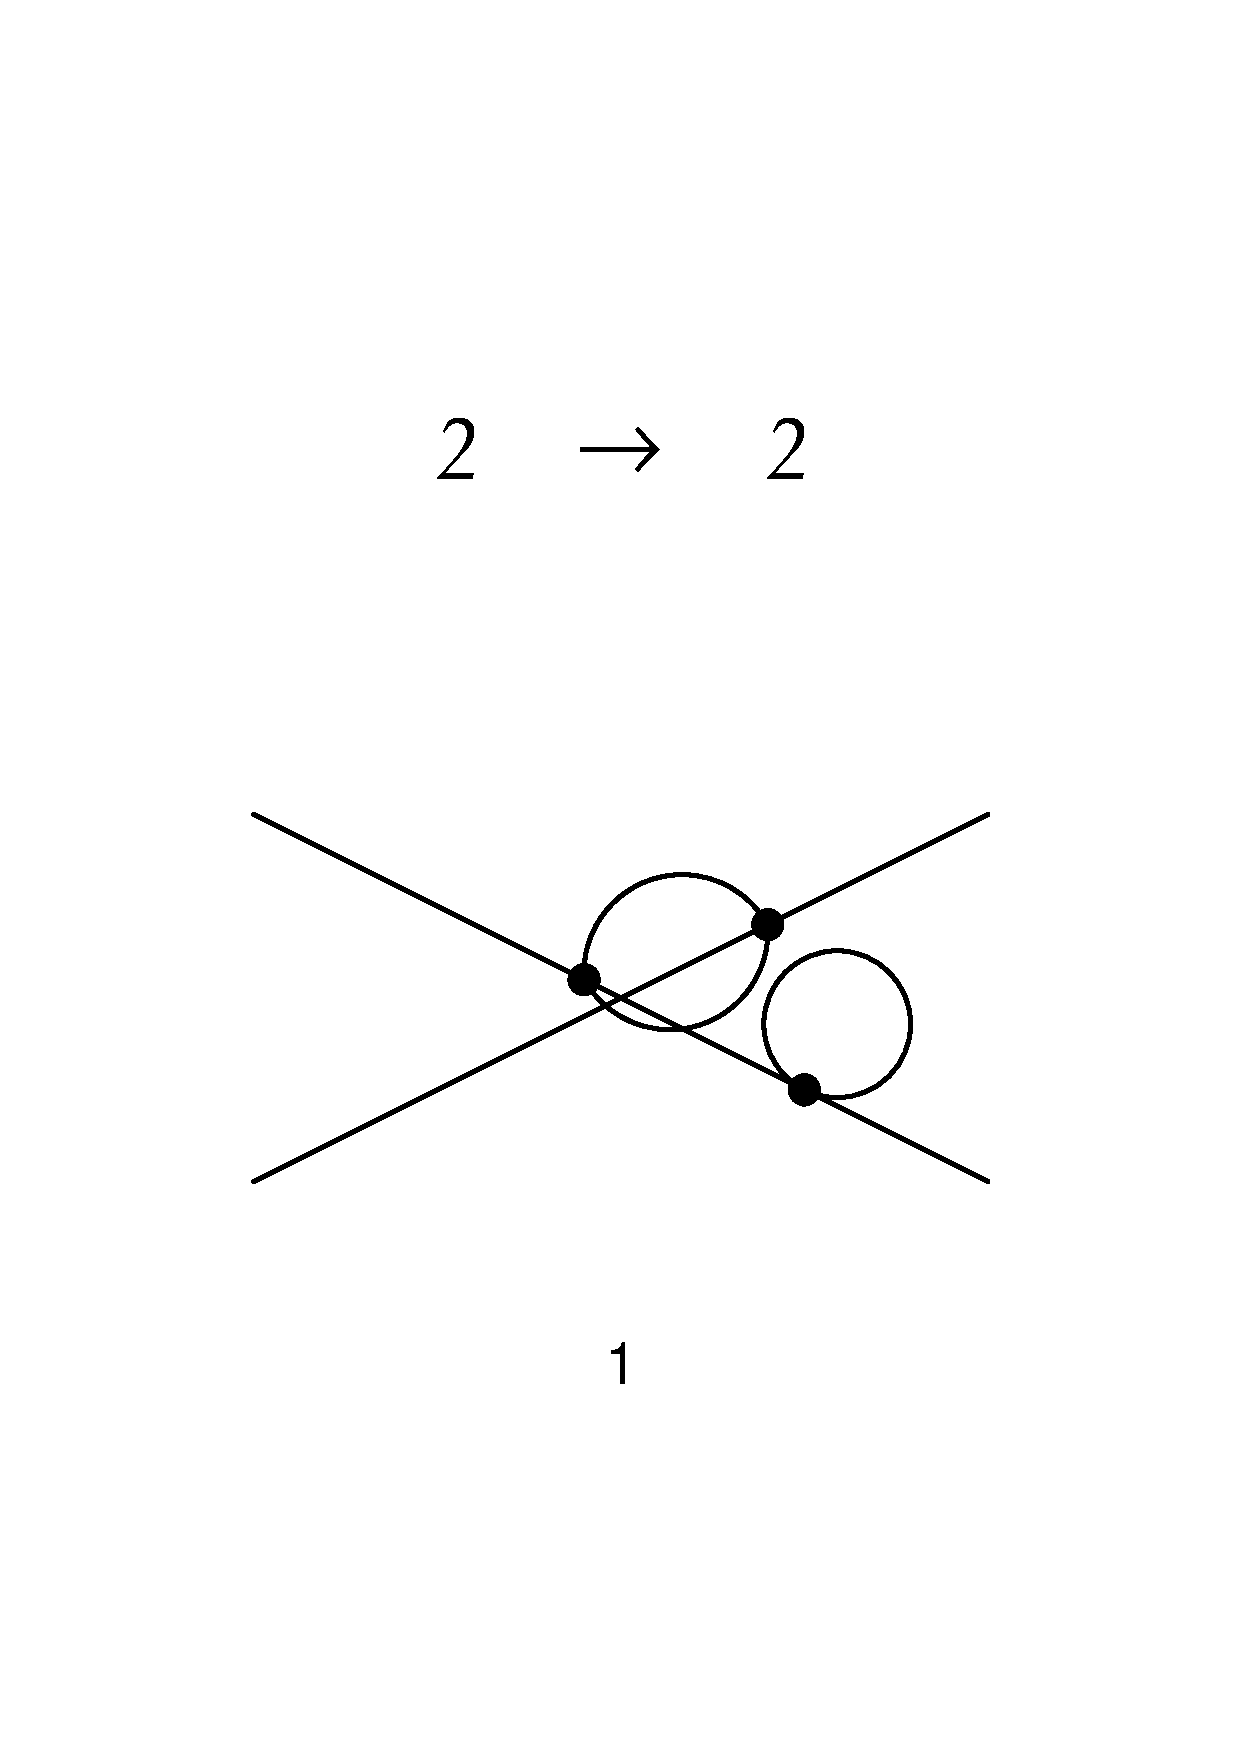
\includegraphics[width=0.28\textwidth]{generated/L2/images/topology16.pdf}
\end{center}
\noindent Parsed propagators: 8. Internal vertices: 3. Internal half-edges: 12.\\
\noindent Assignments checked: 32768. Surviving (nonzero vertex weight): 4096.\\
\noindent Raw $N_c$ power: 1. Net power in $C(t)$: -3.
\noindent Explicit surviving terms:
\begin{equation*}
\mathcal{T}_{16,1} = 128 i g_{2}^{3}\,N_c^{-3}\,G^>\left(x_3,z_{2}\right) \, G^>\left(z_{3},z_{1}\right) \, G_A\left(x_2,z_{2}\right) \, G_A\left(x_4,z_{3}\right) \, G_A\left(z_{1},z_{2}\right) \, G_A\left(z_{3},z_{3}\right) \, G_K\left(x_1,z_{1}\right) \, G_R\left(z_{1},z_{2}\right)
\end{equation*}
\begin{equation*}
\mathcal{T}_{16,2} = 128 i g_{2}^{3}\,N_c^{-3}\,G^>\left(x_3,z_{2}\right) \, G^>\left(z_{3},z_{1}\right) \, G_A\left(x_2,z_{2}\right) \, G_A\left(x_4,z_{3}\right) \, G_A\left(z_{1},z_{2}\right) \, G_K\left(x_1,z_{1}\right) \, G_R\left(z_{1},z_{2}\right) \, G_R\left(z_{3},z_{3}\right)
\end{equation*}
\begin{equation*}
\mathcal{T}_{16,3} = 128 i g_{2}^{3}\,N_c^{-3}\,G^>\left(x_3,z_{2}\right) \, G^>\left(z_{3},z_{1}\right) \, G_A\left(x_2,z_{2}\right) \, G_A\left(x_4,z_{3}\right) \, G_A\left(z_{3},z_{3}\right) \, G_K\left(z_{1},z_{2}\right) \, G_R\left(x_1,z_{1}\right) \, G_R\left(z_{1},z_{2}\right)
\end{equation*}
\begin{equation*}
\mathcal{T}_{16,4} = 128 i g_{2}^{3}\,N_c^{-3}\,G^>\left(x_3,z_{2}\right) \, G^>\left(z_{3},z_{1}\right) \, G_A\left(x_2,z_{2}\right) \, G_A\left(x_4,z_{3}\right) \, G_K\left(z_{1},z_{2}\right) \, G_R\left(x_1,z_{1}\right) \, G_R\left(z_{1},z_{2}\right) \, G_R\left(z_{3},z_{3}\right)
\end{equation*}
\section*{Topology 17 (FeynArts Topology 4)}
\begin{center}
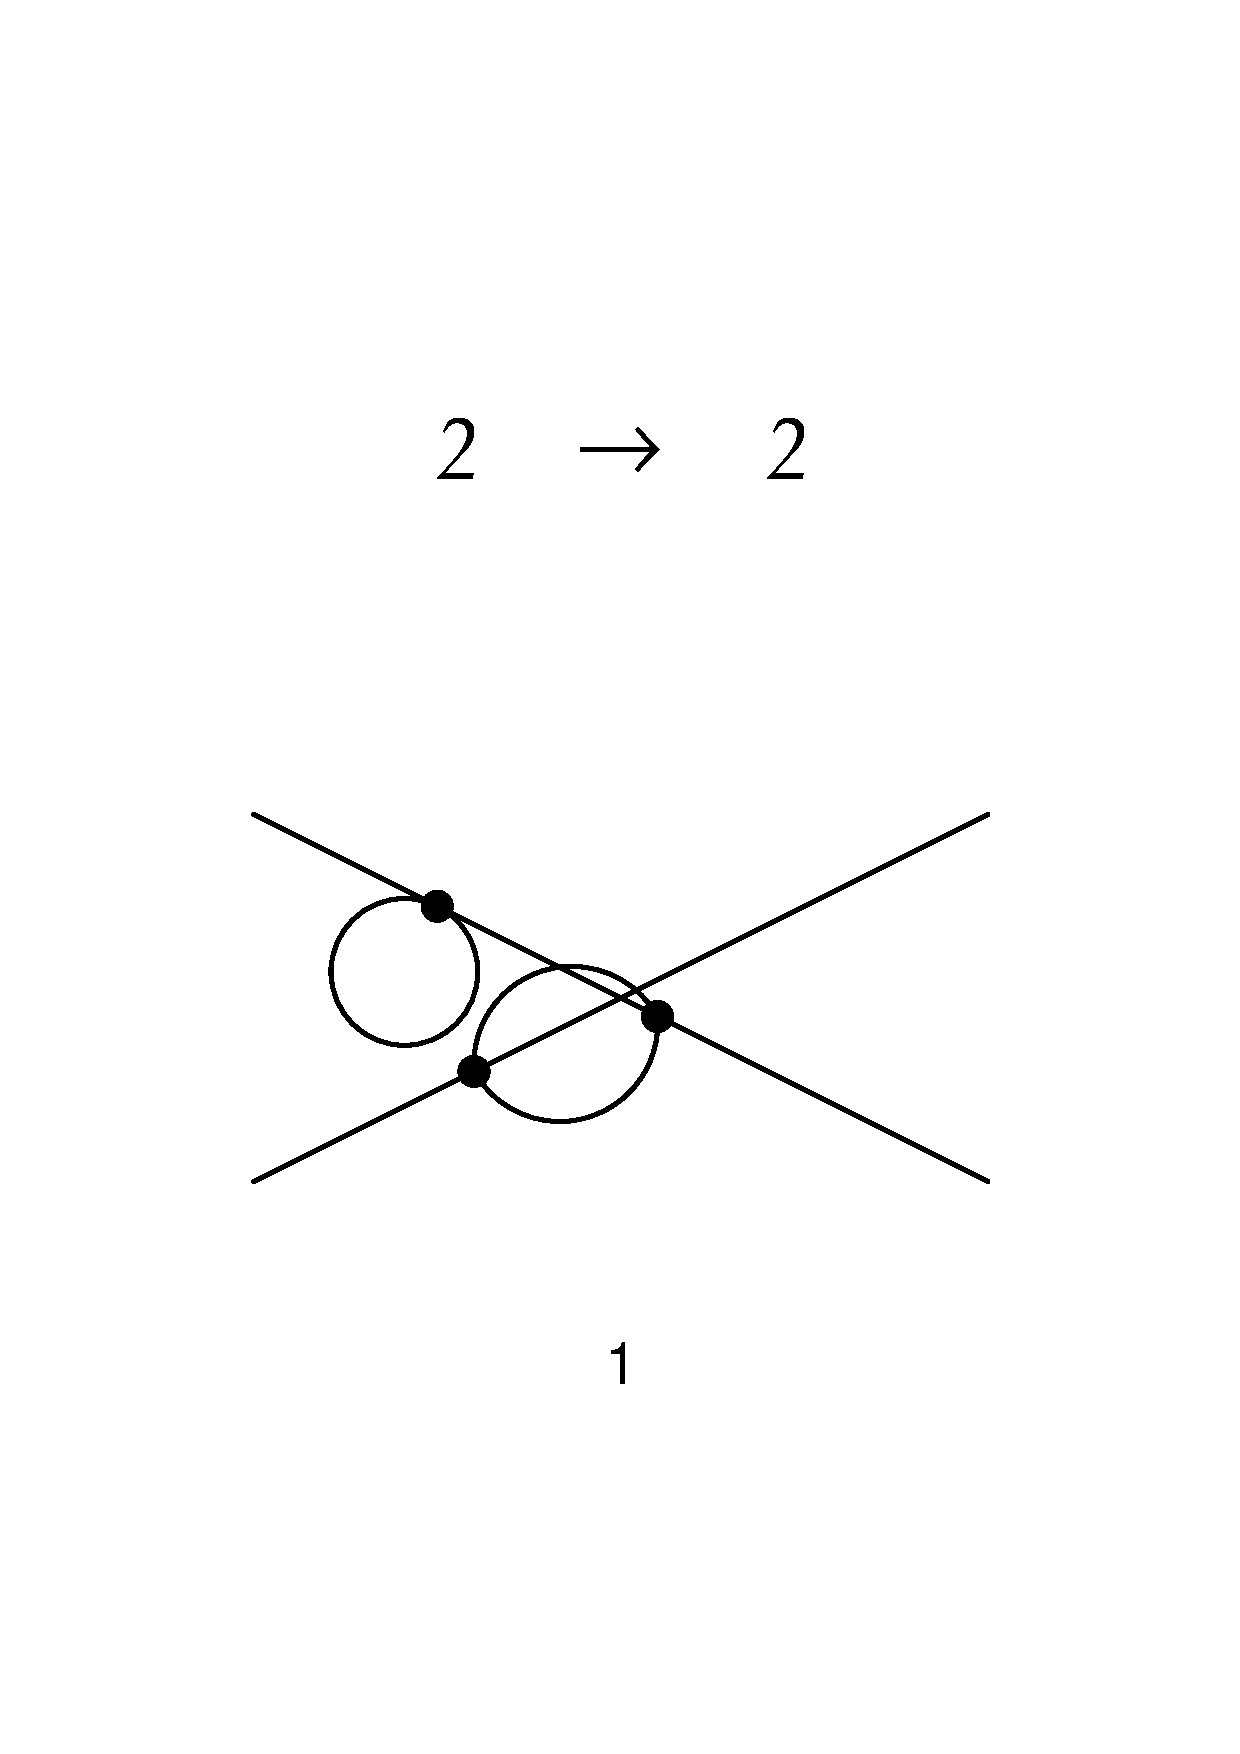
\includegraphics[width=0.28\textwidth]{generated/L2/images/topology17.pdf}
\end{center}
\noindent Parsed propagators: 8. Internal vertices: 3. Internal half-edges: 12.\\
\noindent Assignments checked: 32768. Surviving (nonzero vertex weight): 4096.\\
\noindent Raw $N_c$ power: 1. Net power in $C(t)$: -3.
\[\text{No surviving SK contributions for this topology.}\]
\section*{Topology 18 (FeynArts Topology 4)}
\begin{center}
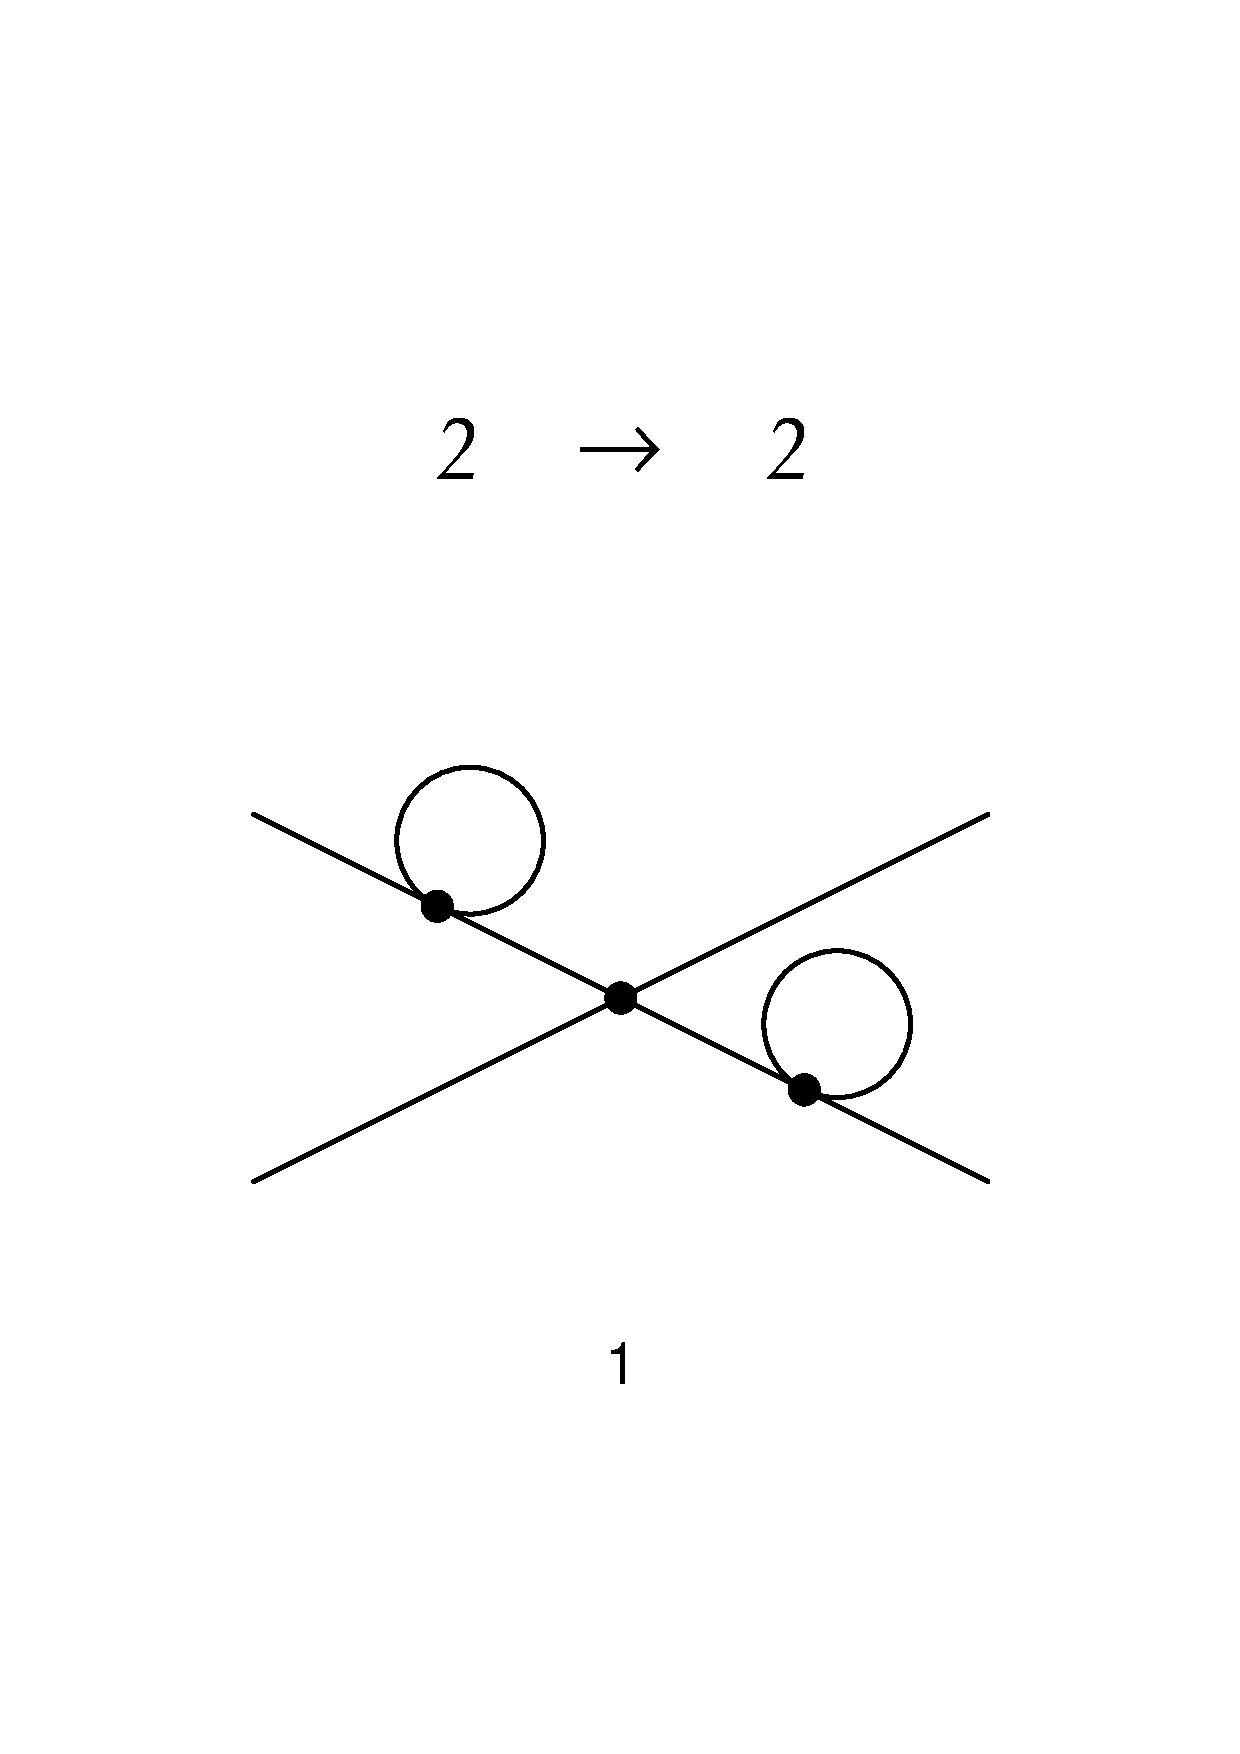
\includegraphics[width=0.28\textwidth]{generated/L2/images/topology18.pdf}
\end{center}
\noindent Parsed propagators: 8. Internal vertices: 3. Internal half-edges: 12.\\
\noindent Assignments checked: 32768. Surviving (nonzero vertex weight): 4096.\\
\noindent Raw $N_c$ power: 2. Net power in $C(t)$: -2.
\noindent Explicit surviving terms:
\begin{equation*}
\mathcal{T}_{18,1} = 64 i g_{2}^{3}\,N_c^{-2}\,G^>\left(x_3,z_{2}\right) \, G^>\left(z_{3},z_{2}\right) \, G_A\left(x_2,z_{2}\right) \, G_A\left(x_4,z_{3}\right) \, G_A\left(z_{1},z_{1}\right) \, G_A\left(z_{3},z_{3}\right) \, G_K\left(x_1,z_{1}\right) \, G_R\left(z_{1},z_{2}\right)
\end{equation*}
\begin{equation*}
\mathcal{T}_{18,2} = 64 i g_{2}^{3}\,N_c^{-2}\,G^>\left(x_3,z_{2}\right) \, G^>\left(z_{3},z_{2}\right) \, G_A\left(x_2,z_{2}\right) \, G_A\left(x_4,z_{3}\right) \, G_A\left(z_{1},z_{1}\right) \, G_K\left(x_1,z_{1}\right) \, G_R\left(z_{1},z_{2}\right) \, G_R\left(z_{3},z_{3}\right)
\end{equation*}
\begin{equation*}
\mathcal{T}_{18,3} = 64 i g_{2}^{3}\,N_c^{-2}\,G^>\left(x_3,z_{2}\right) \, G^>\left(z_{3},z_{2}\right) \, G_A\left(x_2,z_{2}\right) \, G_A\left(x_4,z_{3}\right) \, G_A\left(z_{3},z_{3}\right) \, G_K\left(x_1,z_{1}\right) \, G_R\left(z_{1},z_{1}\right) \, G_R\left(z_{1},z_{2}\right)
\end{equation*}
\begin{equation*}
\mathcal{T}_{18,4} = 64 i g_{2}^{3}\,N_c^{-2}\,G^>\left(x_3,z_{2}\right) \, G^>\left(z_{3},z_{2}\right) \, G_A\left(x_2,z_{2}\right) \, G_A\left(x_4,z_{3}\right) \, G_A\left(z_{3},z_{3}\right) \, G_K\left(z_{1},z_{1}\right) \, G_R\left(x_1,z_{1}\right) \, G_R\left(z_{1},z_{2}\right)
\end{equation*}
\begin{equation*}
\mathcal{T}_{18,5} = 64 i g_{2}^{3}\,N_c^{-2}\,G^>\left(x_3,z_{2}\right) \, G^>\left(z_{3},z_{2}\right) \, G_A\left(x_2,z_{2}\right) \, G_A\left(x_4,z_{3}\right) \, G_K\left(x_1,z_{1}\right) \, G_R\left(z_{1},z_{1}\right) \, G_R\left(z_{1},z_{2}\right) \, G_R\left(z_{3},z_{3}\right)
\end{equation*}
\begin{equation*}
\mathcal{T}_{18,6} = 64 i g_{2}^{3}\,N_c^{-2}\,G^>\left(x_3,z_{2}\right) \, G^>\left(z_{3},z_{2}\right) \, G_A\left(x_2,z_{2}\right) \, G_A\left(x_4,z_{3}\right) \, G_K\left(z_{1},z_{1}\right) \, G_R\left(x_1,z_{1}\right) \, G_R\left(z_{1},z_{2}\right) \, G_R\left(z_{3},z_{3}\right)
\end{equation*}
\section*{Topology 19 (FeynArts Topology 4)}
\begin{center}
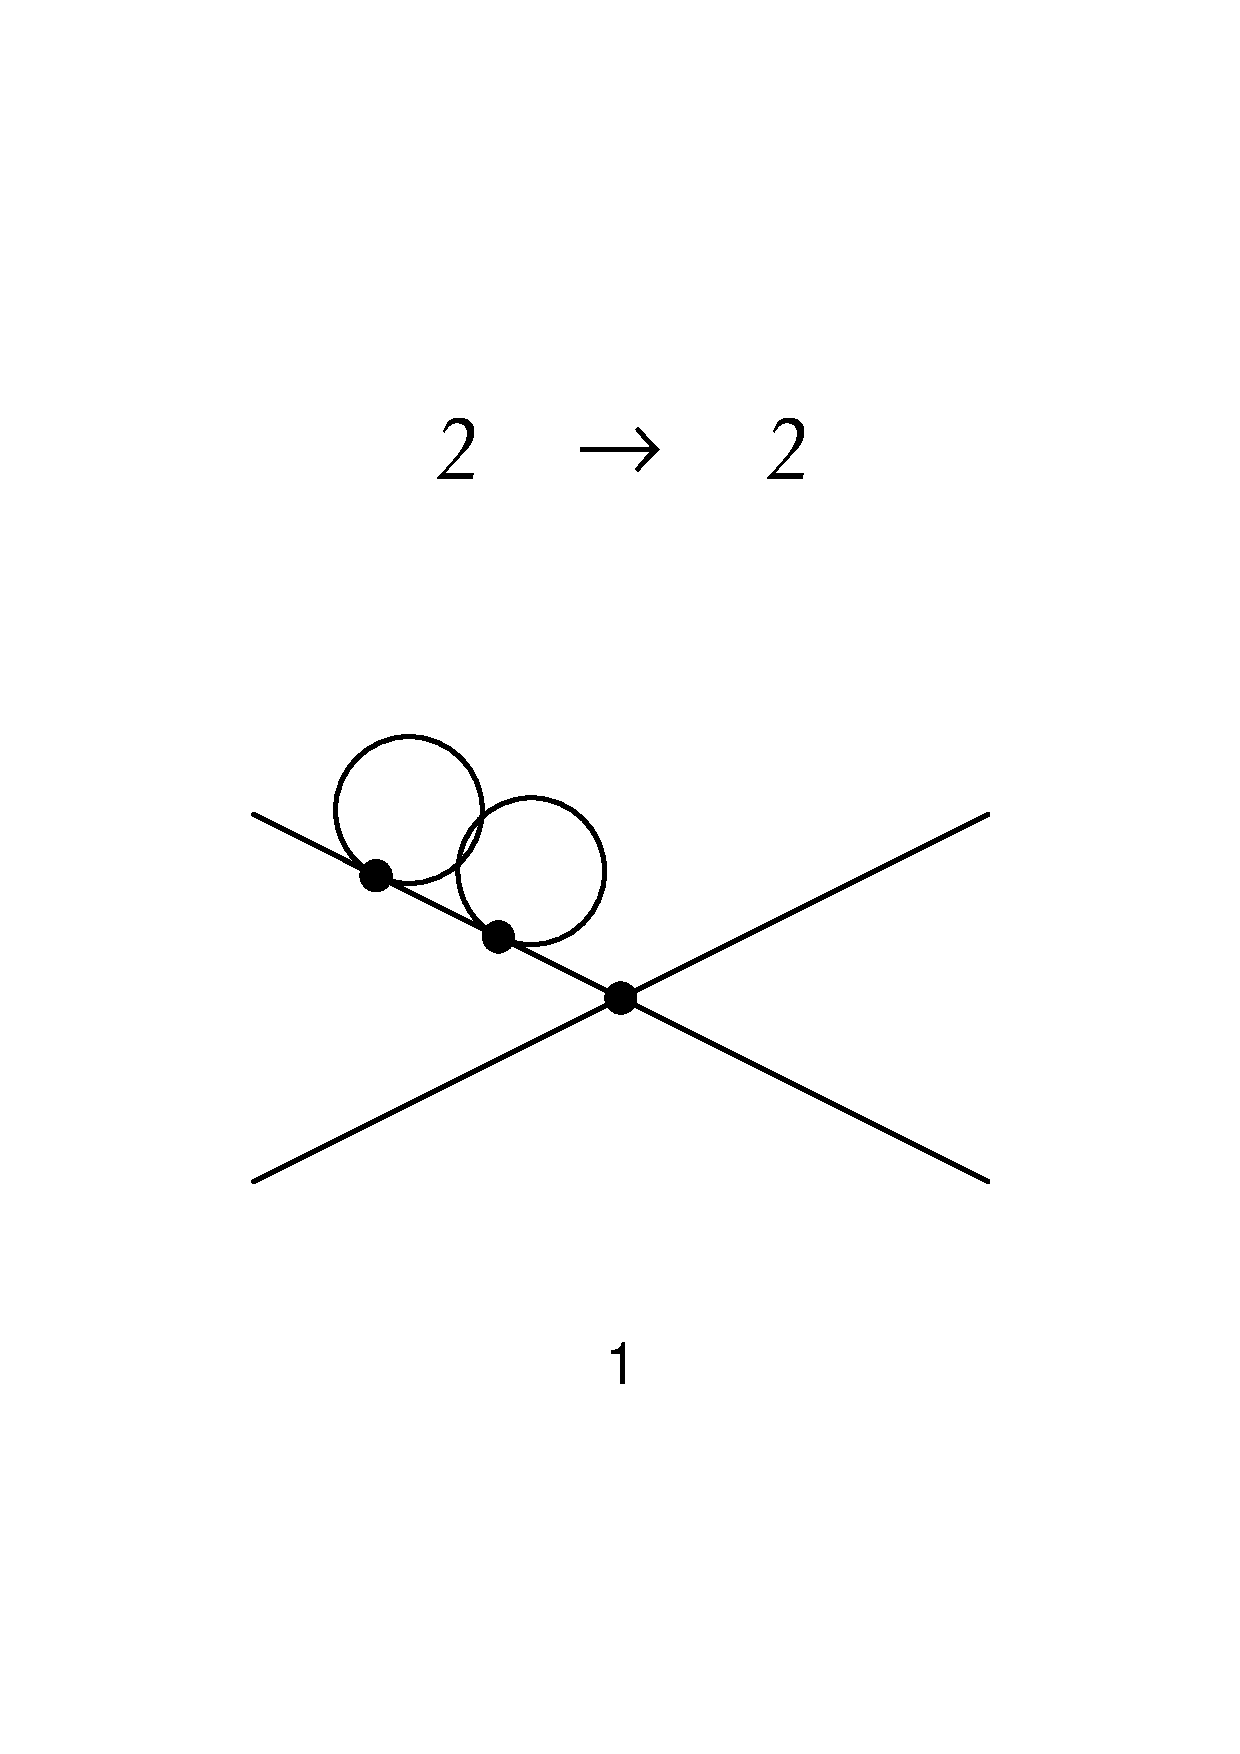
\includegraphics[width=0.28\textwidth]{generated/L2/images/topology19.pdf}
\end{center}
\noindent Parsed propagators: 8. Internal vertices: 3. Internal half-edges: 12.\\
\noindent Assignments checked: 32768. Surviving (nonzero vertex weight): 4096.\\
\noindent Raw $N_c$ power: 2. Net power in $C(t)$: -2.
\[\text{No surviving SK contributions for this topology.}\]
\section*{Topology 20 (FeynArts Topology 4)}
\begin{center}
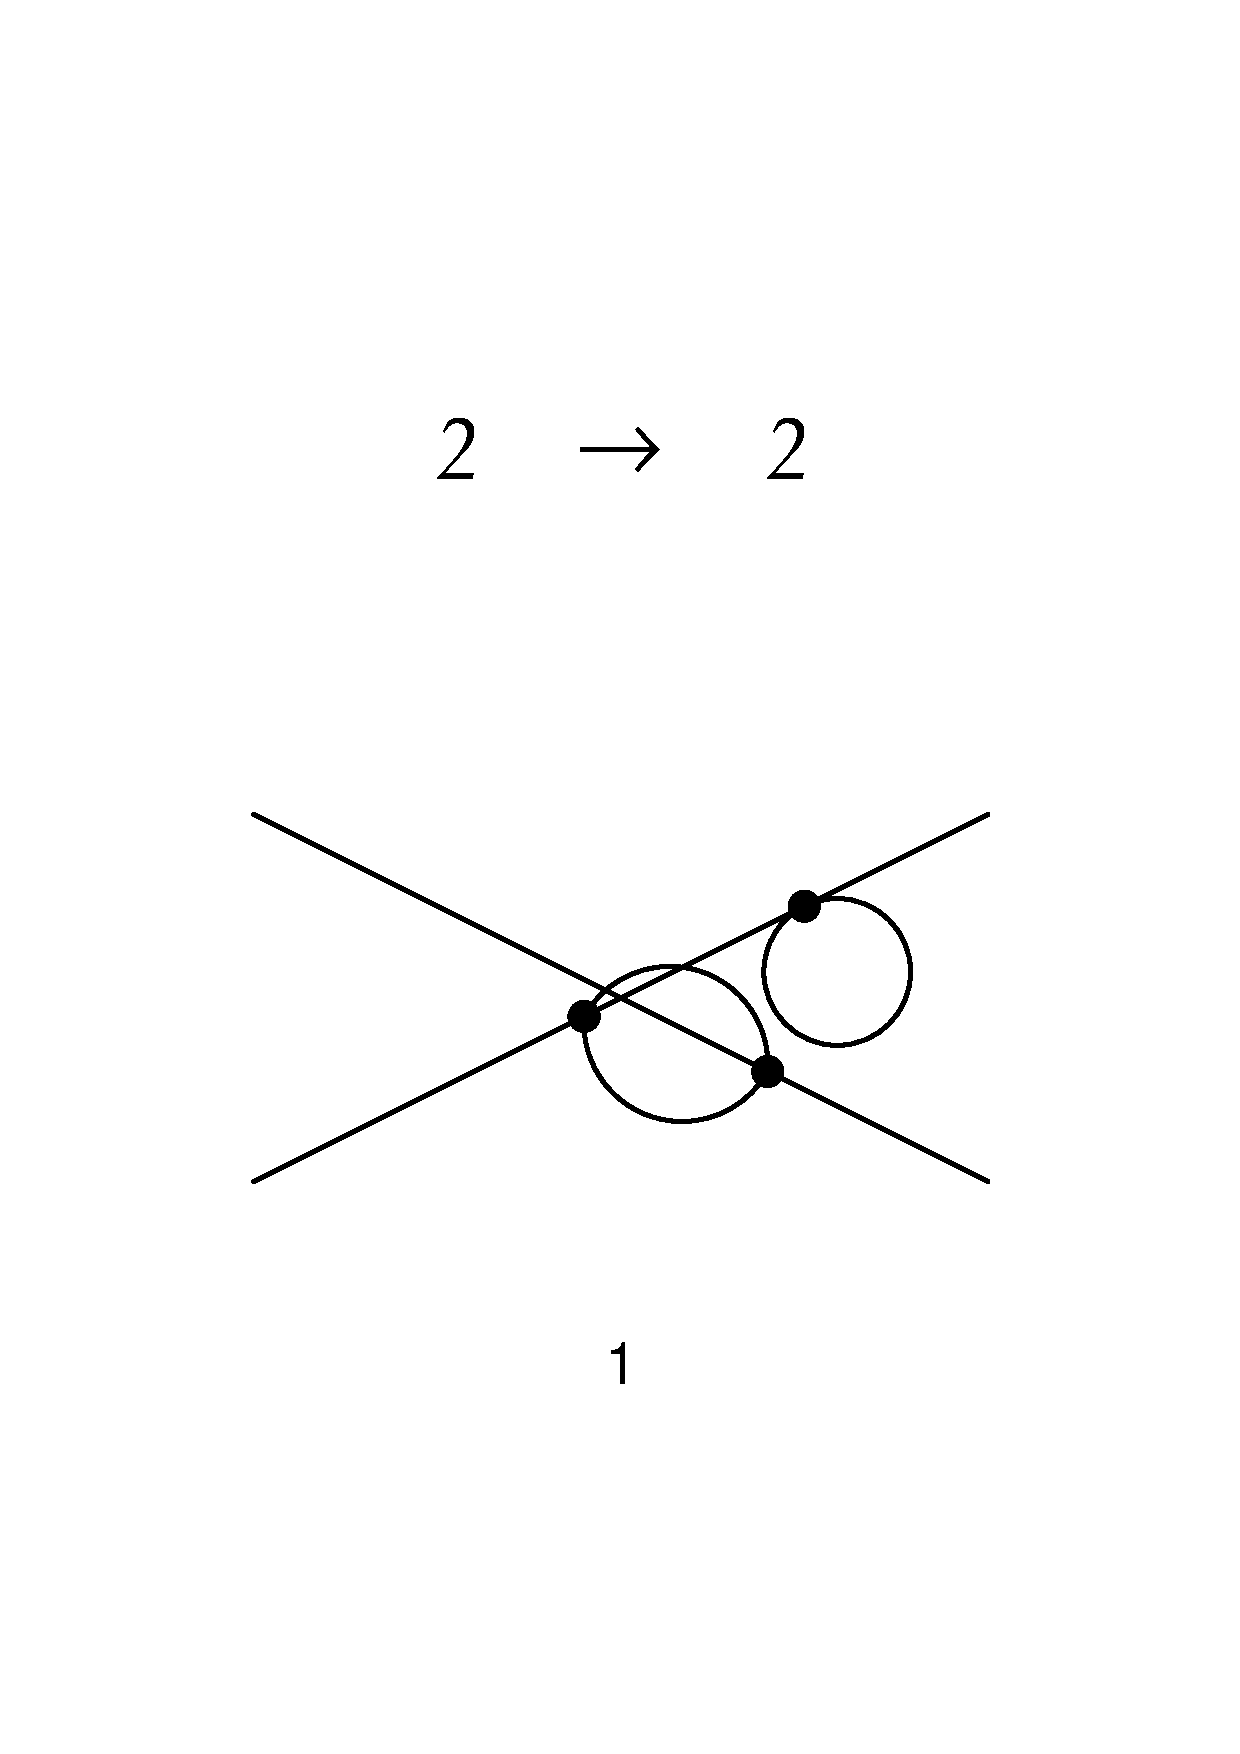
\includegraphics[width=0.28\textwidth]{generated/L2/images/topology20.pdf}
\end{center}
\noindent Parsed propagators: 8. Internal vertices: 3. Internal half-edges: 12.\\
\noindent Assignments checked: 32768. Surviving (nonzero vertex weight): 4096.\\
\noindent Raw $N_c$ power: 1. Net power in $C(t)$: -3.
\[\text{No surviving SK contributions for this topology.}\]
\section*{Topology 21 (FeynArts Topology 4)}
\begin{center}
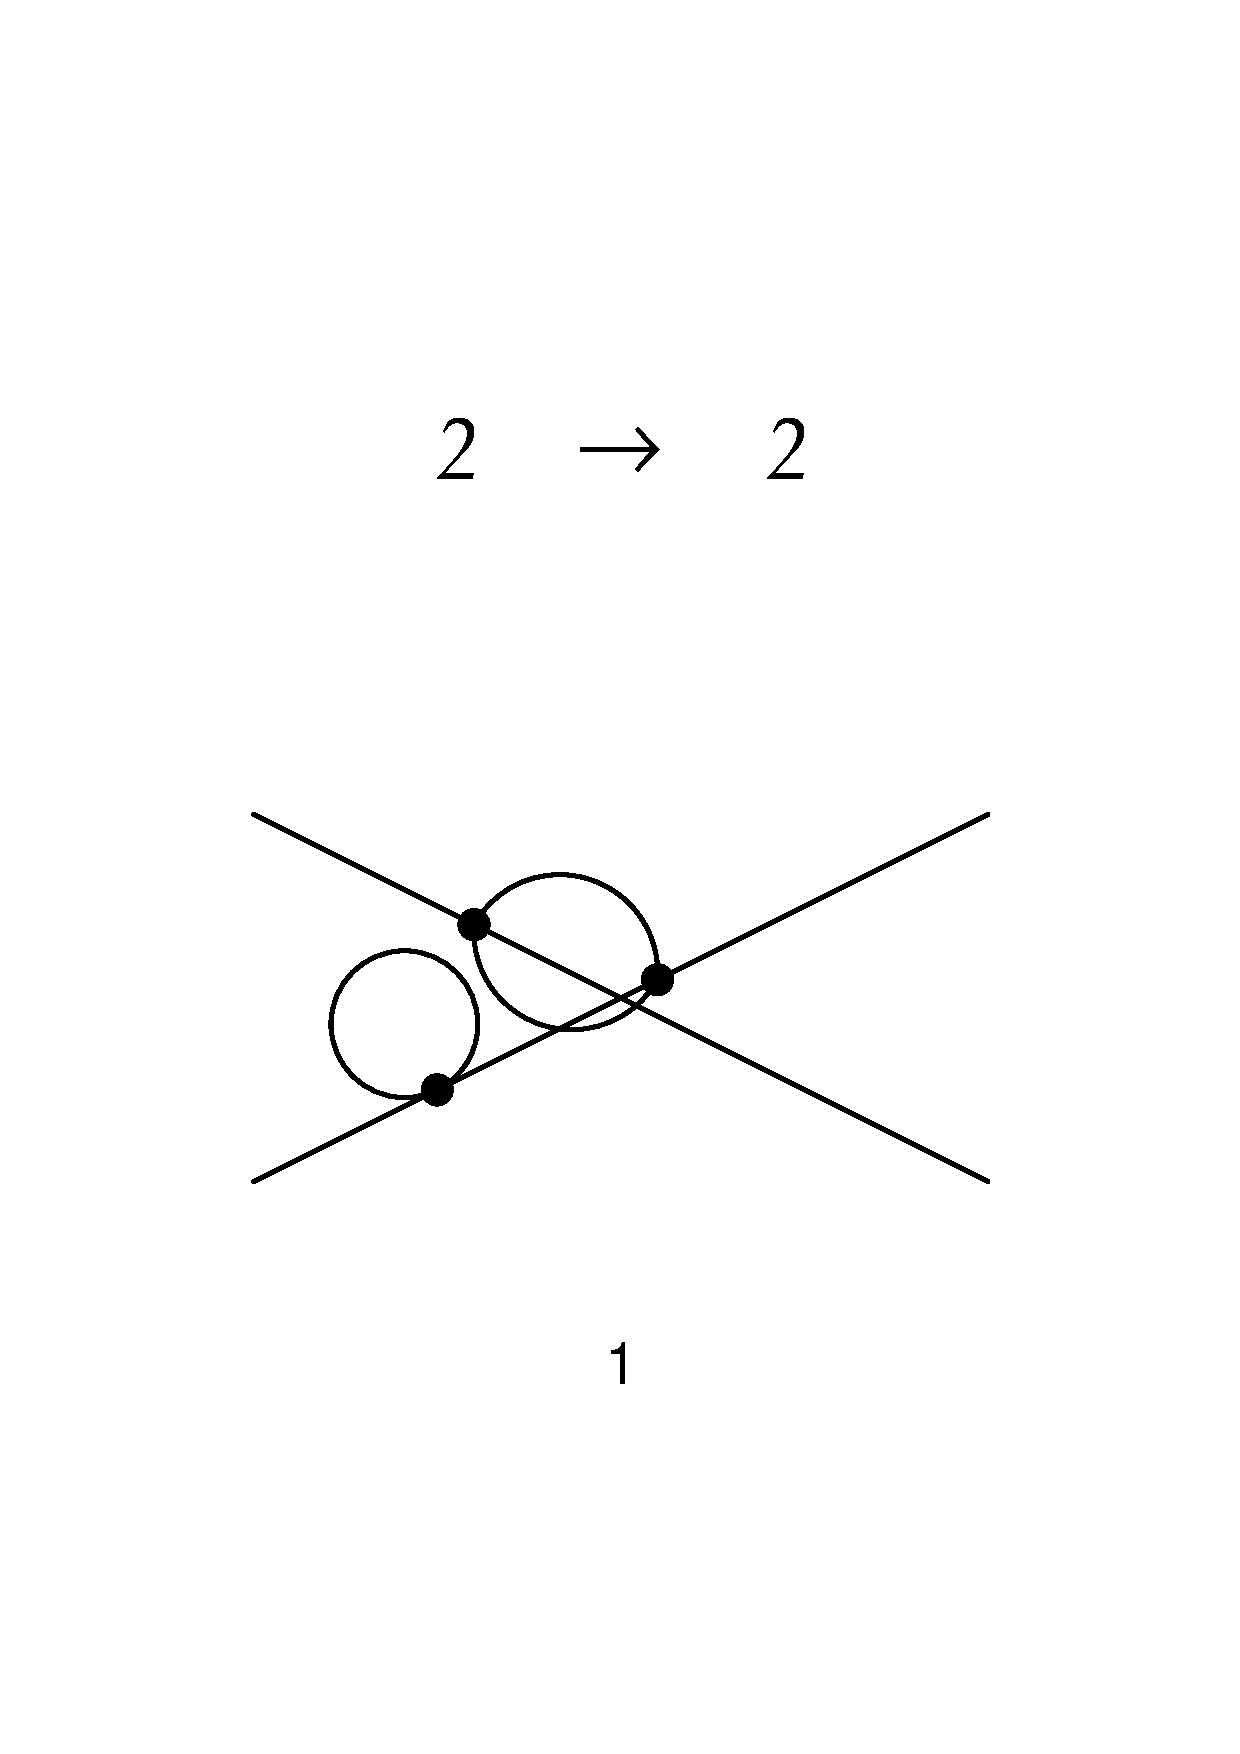
\includegraphics[width=0.28\textwidth]{generated/L2/images/topology21.pdf}
\end{center}
\noindent Parsed propagators: 8. Internal vertices: 3. Internal half-edges: 12.\\
\noindent Assignments checked: 32768. Surviving (nonzero vertex weight): 4096.\\
\noindent Raw $N_c$ power: 1. Net power in $C(t)$: -3.
\noindent Explicit surviving terms:
\begin{equation*}
\mathcal{T}_{21,1} = 128 i g_{2}^{3}\,N_c^{-3}\,G^<\left(x_1,z_{1}\right) \, G^>\left(z_{3},z_{2}\right) \, G_A\left(x_2,z_{2}\right) \, G_A\left(x_4,z_{1}\right) \, G_A\left(z_{2},z_{2}\right) \, G_A\left(z_{3},z_{1}\right) \, G_K\left(x_3,z_{3}\right) \, G_R\left(z_{3},z_{1}\right)
\end{equation*}
\begin{equation*}
\mathcal{T}_{21,2} = 128 i g_{2}^{3}\,N_c^{-3}\,G^<\left(x_1,z_{1}\right) \, G^>\left(z_{3},z_{2}\right) \, G_A\left(x_2,z_{2}\right) \, G_A\left(x_4,z_{1}\right) \, G_A\left(z_{2},z_{2}\right) \, G_K\left(z_{3},z_{1}\right) \, G_R\left(x_3,z_{3}\right) \, G_R\left(z_{3},z_{1}\right)
\end{equation*}
\begin{equation*}
\mathcal{T}_{21,3} = 128 i g_{2}^{3}\,N_c^{-3}\,G^<\left(x_1,z_{1}\right) \, G^>\left(z_{3},z_{2}\right) \, G_A\left(x_2,z_{2}\right) \, G_A\left(x_4,z_{1}\right) \, G_A\left(z_{3},z_{1}\right) \, G_K\left(x_3,z_{3}\right) \, G_R\left(z_{2},z_{2}\right) \, G_R\left(z_{3},z_{1}\right)
\end{equation*}
\begin{equation*}
\mathcal{T}_{21,4} = 128 i g_{2}^{3}\,N_c^{-3}\,G^<\left(x_1,z_{1}\right) \, G^>\left(z_{3},z_{2}\right) \, G_A\left(x_2,z_{2}\right) \, G_A\left(x_4,z_{1}\right) \, G_K\left(z_{3},z_{1}\right) \, G_R\left(x_3,z_{3}\right) \, G_R\left(z_{2},z_{2}\right) \, G_R\left(z_{3},z_{1}\right)
\end{equation*}
\section*{Topology 22 (FeynArts Topology 4)}
\begin{center}
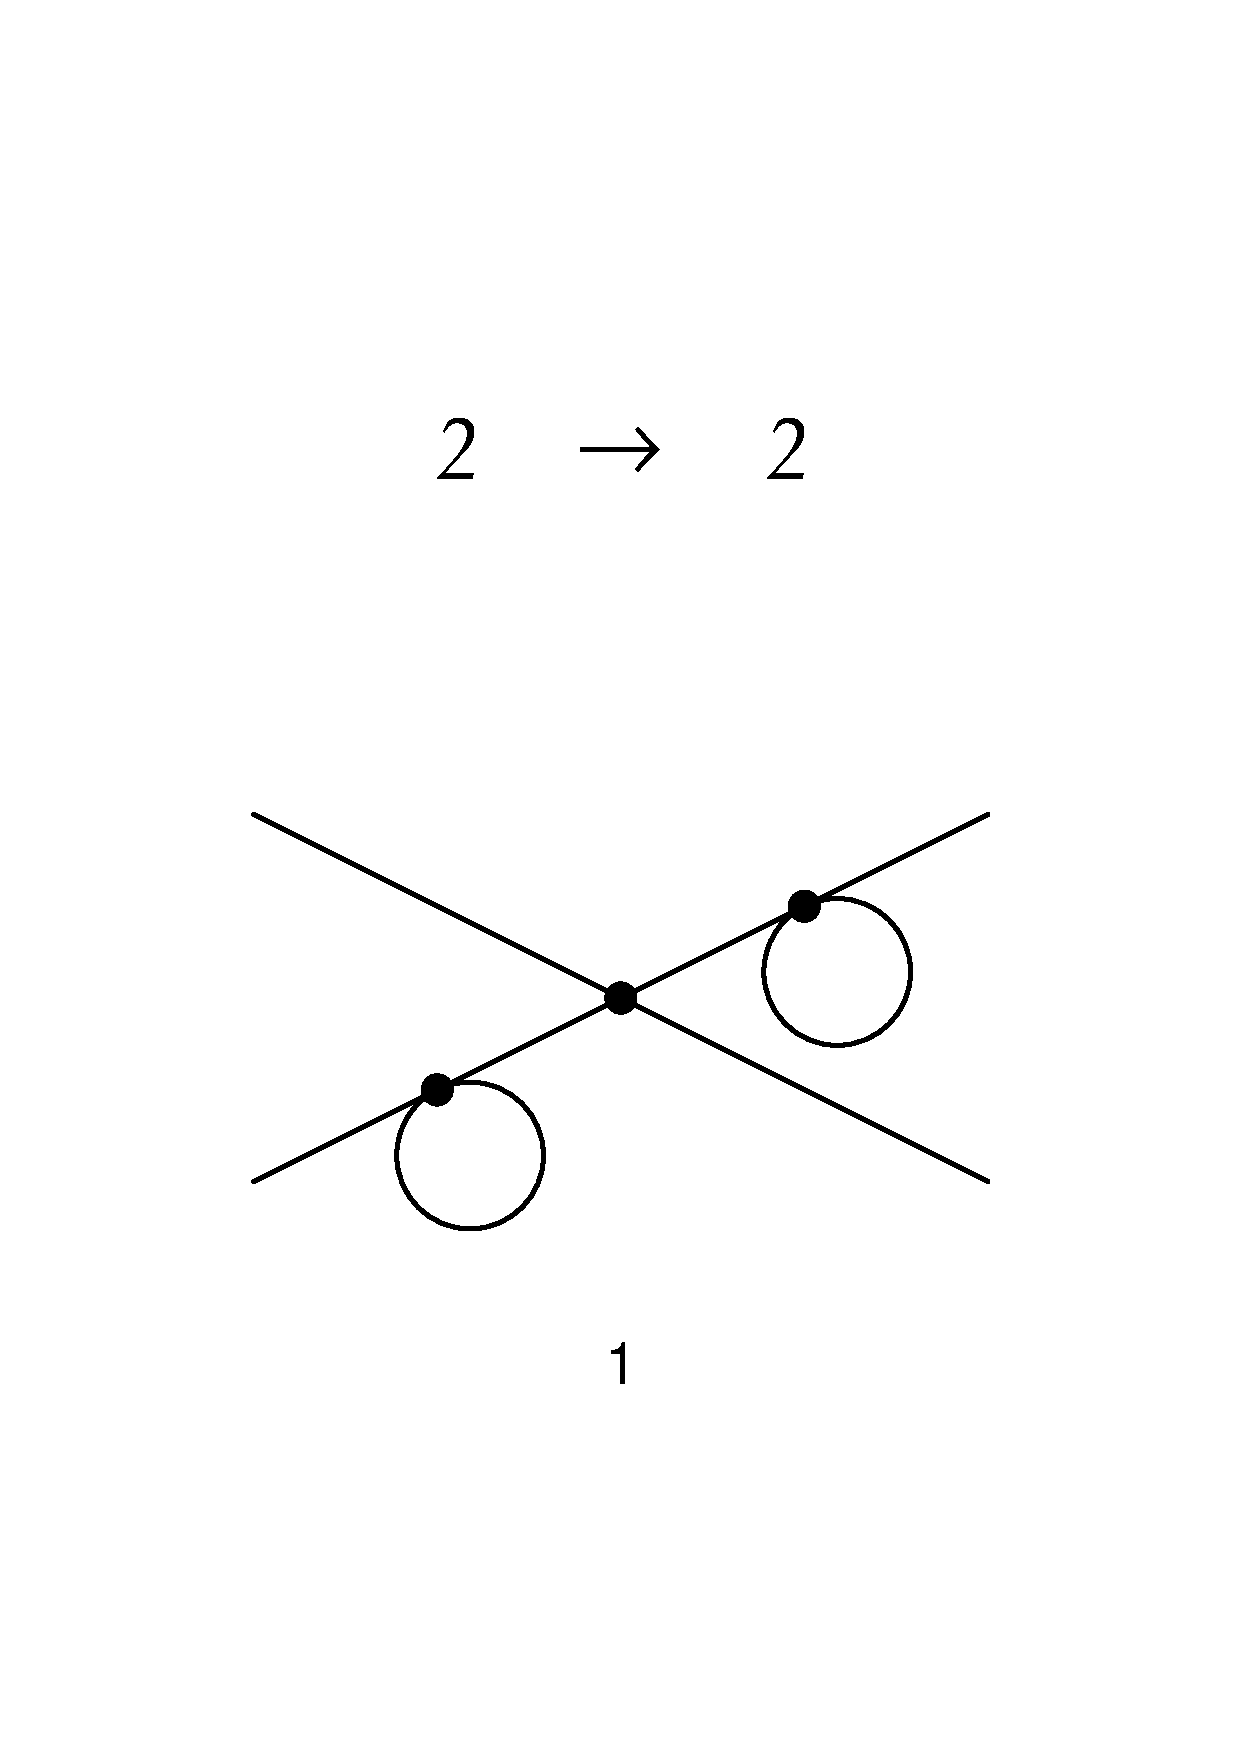
\includegraphics[width=0.28\textwidth]{generated/L2/images/topology22.pdf}
\end{center}
\noindent Parsed propagators: 8. Internal vertices: 3. Internal half-edges: 12.\\
\noindent Assignments checked: 32768. Surviving (nonzero vertex weight): 4096.\\
\noindent Raw $N_c$ power: 2. Net power in $C(t)$: -2.
\noindent Explicit surviving terms:
\begin{equation*}
\mathcal{T}_{22,1} = 64 i g_{2}^{3}\,N_c^{-2}\,G^<\left(x_1,z_{1}\right) \, G^<\left(z_{2},z_{1}\right) \, G_A\left(x_2,z_{2}\right) \, G_A\left(x_4,z_{1}\right) \, G_A\left(z_{2},z_{2}\right) \, G_A\left(z_{3},z_{3}\right) \, G_K\left(x_3,z_{3}\right) \, G_R\left(z_{3},z_{1}\right)
\end{equation*}
\begin{equation*}
\mathcal{T}_{22,2} = 64 i g_{2}^{3}\,N_c^{-2}\,G^<\left(x_1,z_{1}\right) \, G^<\left(z_{2},z_{1}\right) \, G_A\left(x_2,z_{2}\right) \, G_A\left(x_4,z_{1}\right) \, G_A\left(z_{2},z_{2}\right) \, G_K\left(x_3,z_{3}\right) \, G_R\left(z_{3},z_{1}\right) \, G_R\left(z_{3},z_{3}\right)
\end{equation*}
\begin{equation*}
\mathcal{T}_{22,3} = 64 i g_{2}^{3}\,N_c^{-2}\,G^<\left(x_1,z_{1}\right) \, G^<\left(z_{2},z_{1}\right) \, G_A\left(x_2,z_{2}\right) \, G_A\left(x_4,z_{1}\right) \, G_A\left(z_{2},z_{2}\right) \, G_K\left(z_{3},z_{3}\right) \, G_R\left(x_3,z_{3}\right) \, G_R\left(z_{3},z_{1}\right)
\end{equation*}
\begin{equation*}
\mathcal{T}_{22,4} = 64 i g_{2}^{3}\,N_c^{-2}\,G^<\left(x_1,z_{1}\right) \, G^<\left(z_{2},z_{1}\right) \, G_A\left(x_2,z_{2}\right) \, G_A\left(x_4,z_{1}\right) \, G_A\left(z_{3},z_{3}\right) \, G_K\left(x_3,z_{3}\right) \, G_R\left(z_{2},z_{2}\right) \, G_R\left(z_{3},z_{1}\right)
\end{equation*}
\begin{equation*}
\mathcal{T}_{22,5} = 64 i g_{2}^{3}\,N_c^{-2}\,G^<\left(x_1,z_{1}\right) \, G^<\left(z_{2},z_{1}\right) \, G_A\left(x_2,z_{2}\right) \, G_A\left(x_4,z_{1}\right) \, G_K\left(x_3,z_{3}\right) \, G_R\left(z_{2},z_{2}\right) \, G_R\left(z_{3},z_{1}\right) \, G_R\left(z_{3},z_{3}\right)
\end{equation*}
\begin{equation*}
\mathcal{T}_{22,6} = 64 i g_{2}^{3}\,N_c^{-2}\,G^<\left(x_1,z_{1}\right) \, G^<\left(z_{2},z_{1}\right) \, G_A\left(x_2,z_{2}\right) \, G_A\left(x_4,z_{1}\right) \, G_K\left(z_{3},z_{3}\right) \, G_R\left(x_3,z_{3}\right) \, G_R\left(z_{2},z_{2}\right) \, G_R\left(z_{3},z_{1}\right)
\end{equation*}
\section*{Topology 23 (FeynArts Topology 4)}
\begin{center}
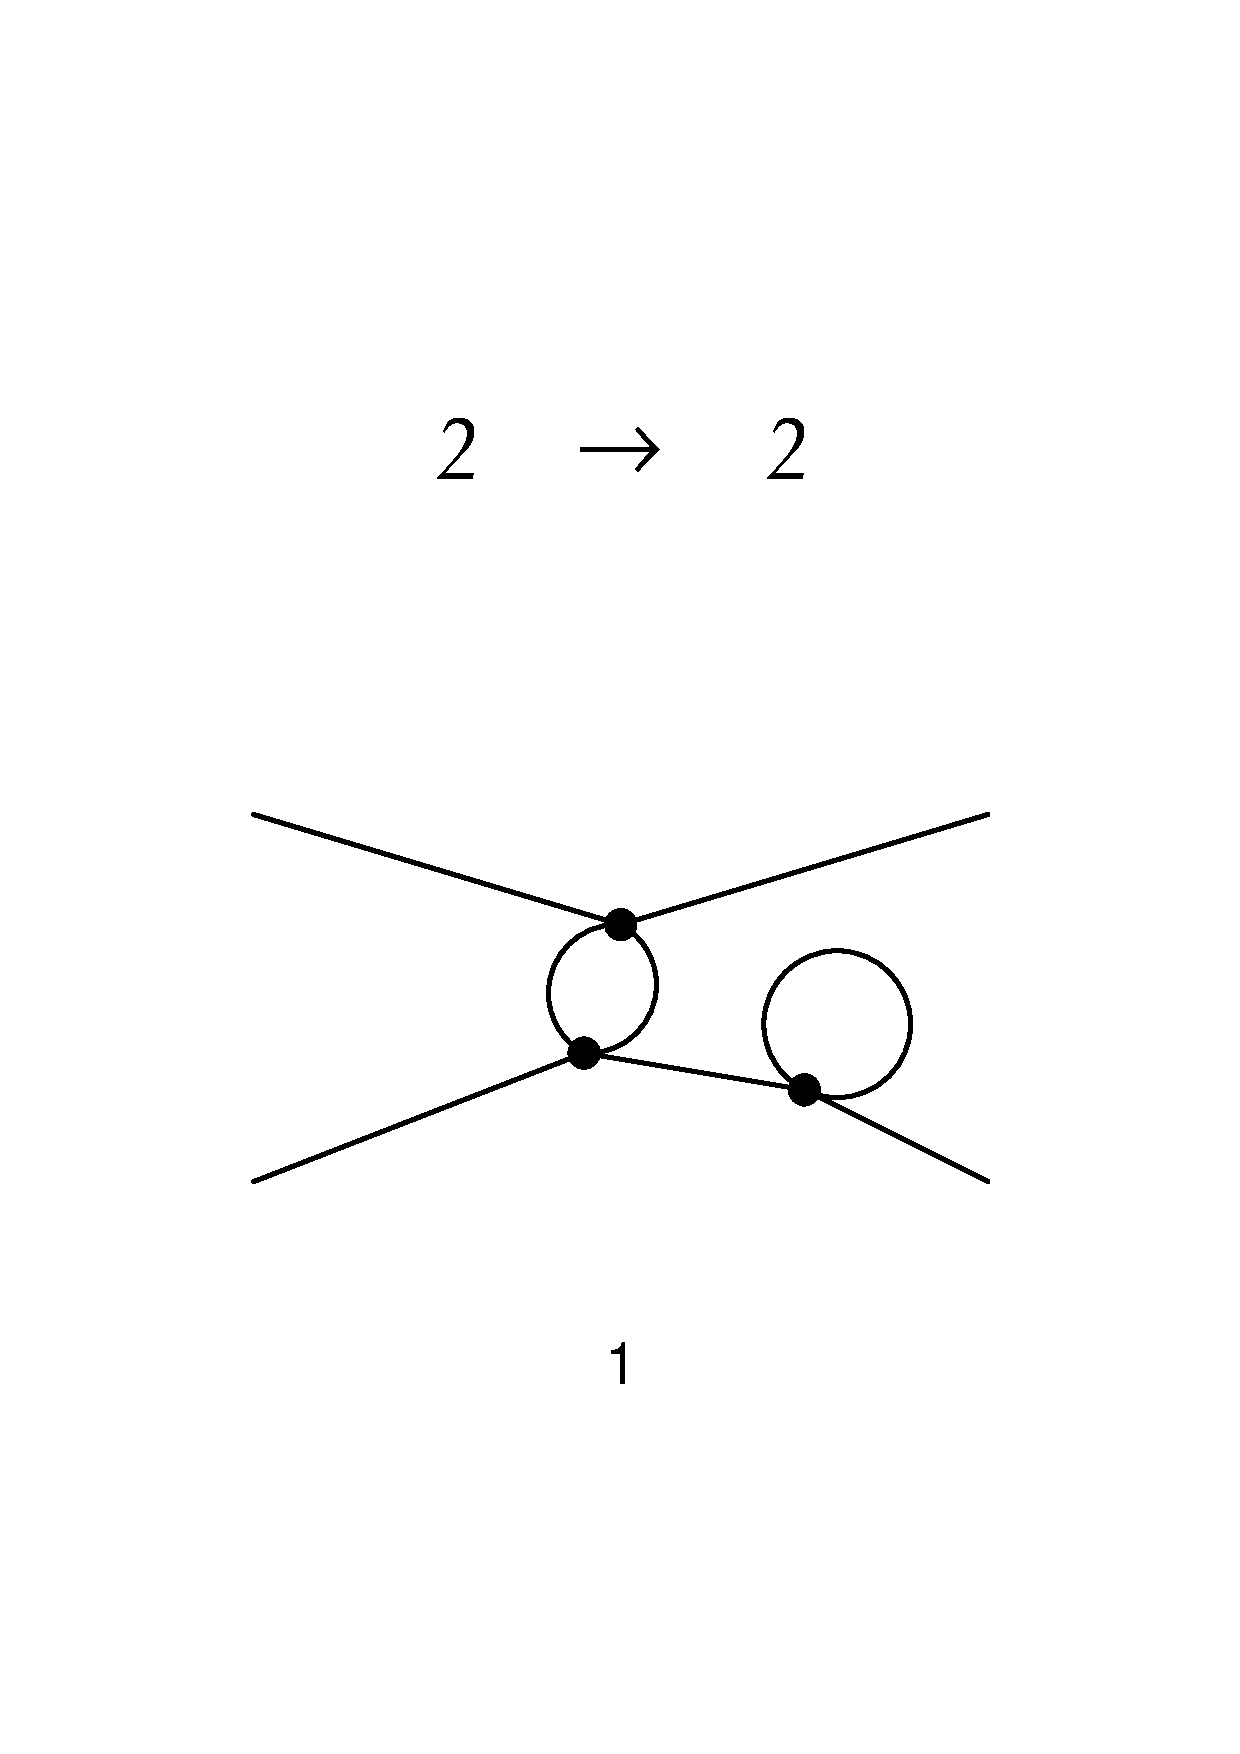
\includegraphics[width=0.28\textwidth]{generated/L2/images/topology23.pdf}
\end{center}
\noindent Parsed propagators: 8. Internal vertices: 3. Internal half-edges: 12.\\
\noindent Assignments checked: 32768. Surviving (nonzero vertex weight): 4096.\\
\noindent Raw $N_c$ power: 1. Net power in $C(t)$: -3.
\noindent Explicit surviving terms:
\begin{equation*}
\mathcal{T}_{23,1} = 128 i g_{2}^{3}\,N_c^{-3}\,G^>\left(x_3,z_{1}\right) \, G^>\left(z_{3},z_{2}\right) \, G_A\left(x_2,z_{2}\right) \, G_A\left(x_4,z_{3}\right) \, G_A\left(z_{2},z_{1}\right) \, G_A\left(z_{3},z_{3}\right) \, G_K\left(x_1,z_{1}\right) \, G_R\left(z_{2},z_{1}\right)
\end{equation*}
\begin{equation*}
\mathcal{T}_{23,2} = 128 i g_{2}^{3}\,N_c^{-3}\,G^>\left(x_3,z_{1}\right) \, G^>\left(z_{3},z_{2}\right) \, G_A\left(x_2,z_{2}\right) \, G_A\left(x_4,z_{3}\right) \, G_A\left(z_{2},z_{1}\right) \, G_A\left(z_{3},z_{3}\right) \, G_K\left(z_{2},z_{1}\right) \, G_R\left(x_1,z_{1}\right)
\end{equation*}
\begin{equation*}
\mathcal{T}_{23,3} = 128 i g_{2}^{3}\,N_c^{-3}\,G^>\left(x_3,z_{1}\right) \, G^>\left(z_{3},z_{2}\right) \, G_A\left(x_2,z_{2}\right) \, G_A\left(x_4,z_{3}\right) \, G_A\left(z_{2},z_{1}\right) \, G_K\left(x_1,z_{1}\right) \, G_R\left(z_{2},z_{1}\right) \, G_R\left(z_{3},z_{3}\right)
\end{equation*}
\begin{equation*}
\mathcal{T}_{23,4} = 128 i g_{2}^{3}\,N_c^{-3}\,G^>\left(x_3,z_{1}\right) \, G^>\left(z_{3},z_{2}\right) \, G_A\left(x_2,z_{2}\right) \, G_A\left(x_4,z_{3}\right) \, G_A\left(z_{2},z_{1}\right) \, G_K\left(z_{2},z_{1}\right) \, G_R\left(x_1,z_{1}\right) \, G_R\left(z_{3},z_{3}\right)
\end{equation*}
\section*{Topology 24 (FeynArts Topology 4)}
\begin{center}
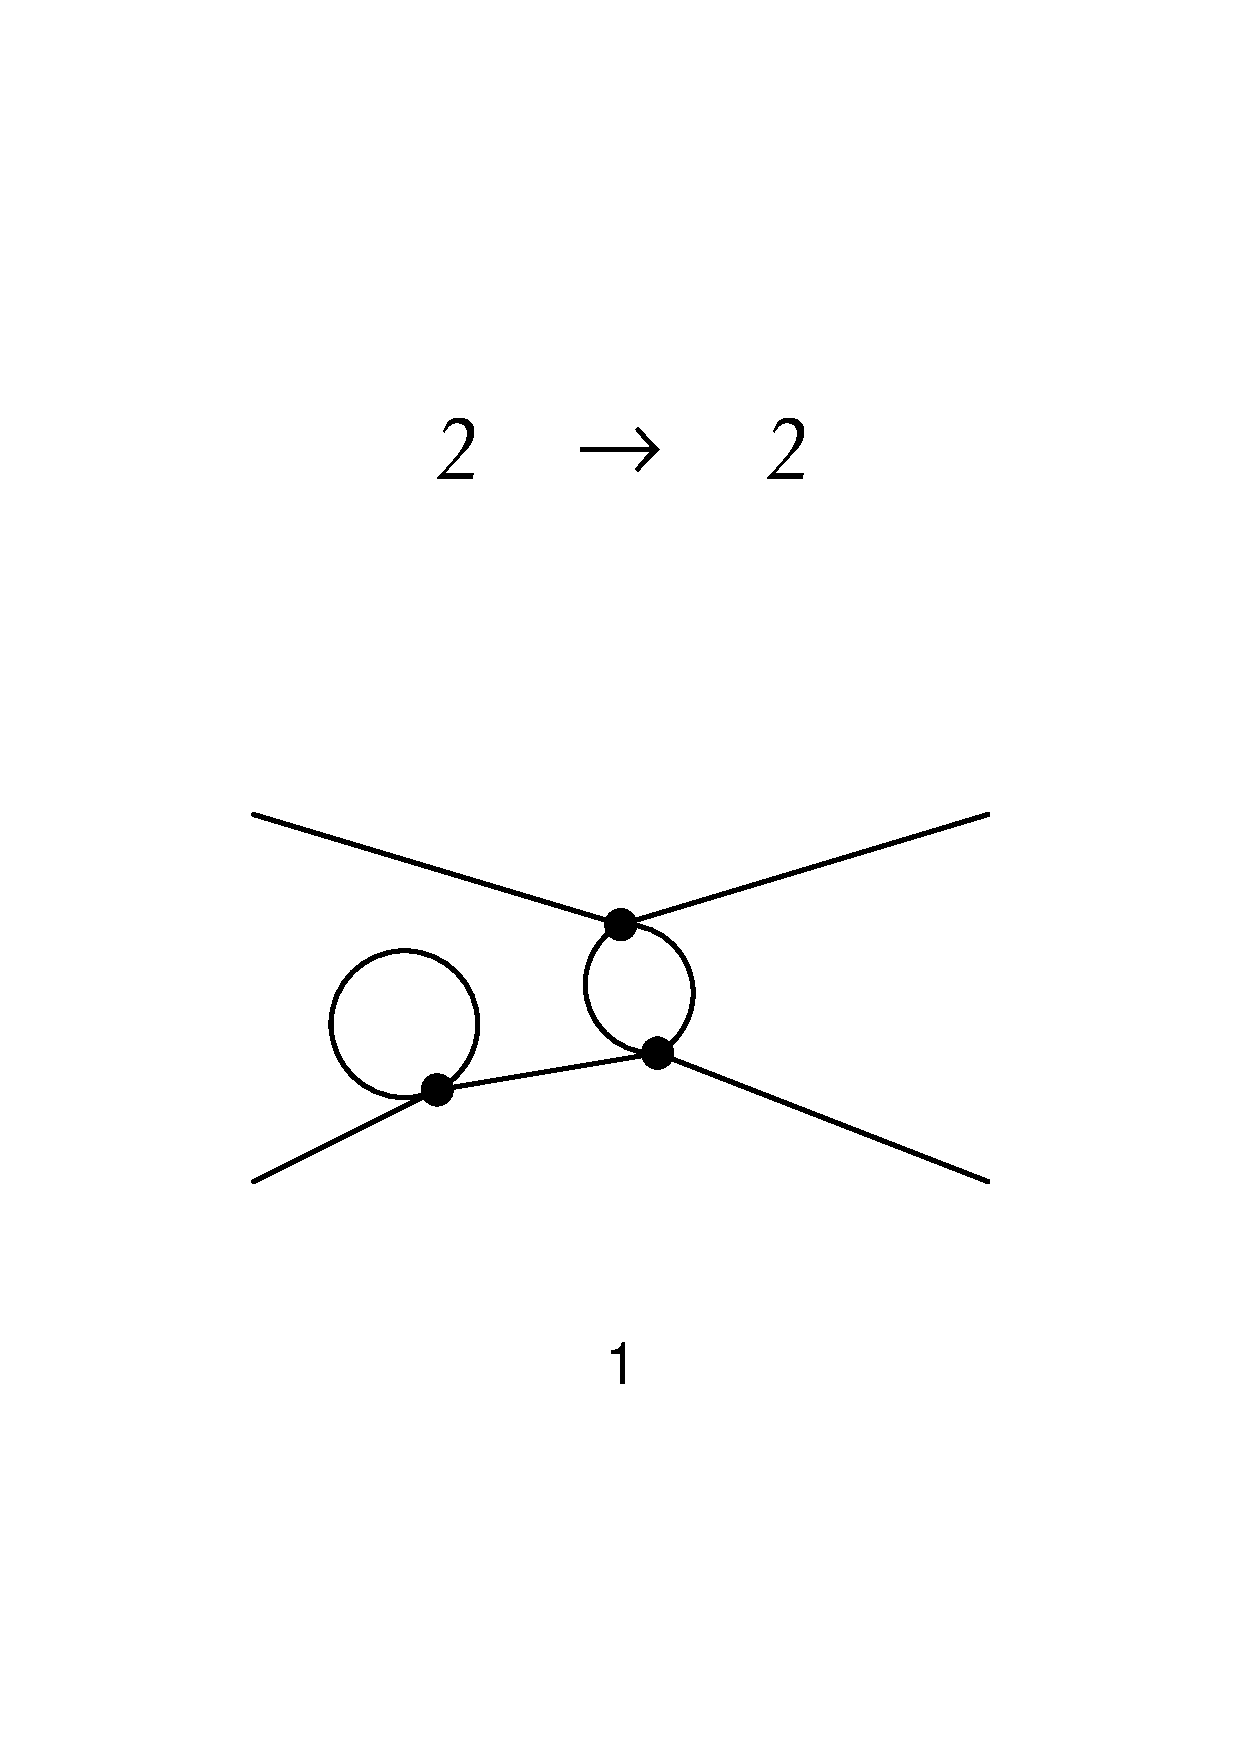
\includegraphics[width=0.28\textwidth]{generated/L2/images/topology24.pdf}
\end{center}
\noindent Parsed propagators: 8. Internal vertices: 3. Internal half-edges: 12.\\
\noindent Assignments checked: 32768. Surviving (nonzero vertex weight): 4096.\\
\noindent Raw $N_c$ power: 1. Net power in $C(t)$: -3.
\noindent Explicit surviving terms:
\begin{equation*}
\mathcal{T}_{24,1} = 128 i g_{2}^{3}\,N_c^{-3}\,G^<\left(x_1,z_{1}\right) \, G^>\left(z_{3},z_{2}\right) \, G_A\left(x_2,z_{2}\right) \, G_A\left(x_4,z_{3}\right) \, G_A\left(z_{2},z_{2}\right) \, G_A\left(z_{3},z_{1}\right) \, G_K\left(x_3,z_{1}\right) \, G_R\left(z_{3},z_{1}\right)
\end{equation*}
\begin{equation*}
\mathcal{T}_{24,2} = 128 i g_{2}^{3}\,N_c^{-3}\,G^<\left(x_1,z_{1}\right) \, G^>\left(z_{3},z_{2}\right) \, G_A\left(x_2,z_{2}\right) \, G_A\left(x_4,z_{3}\right) \, G_A\left(z_{2},z_{2}\right) \, G_A\left(z_{3},z_{1}\right) \, G_K\left(z_{3},z_{1}\right) \, G_R\left(x_3,z_{1}\right)
\end{equation*}
\begin{equation*}
\mathcal{T}_{24,3} = 128 i g_{2}^{3}\,N_c^{-3}\,G^<\left(x_1,z_{1}\right) \, G^>\left(z_{3},z_{2}\right) \, G_A\left(x_2,z_{2}\right) \, G_A\left(x_4,z_{3}\right) \, G_A\left(z_{3},z_{1}\right) \, G_K\left(x_3,z_{1}\right) \, G_R\left(z_{2},z_{2}\right) \, G_R\left(z_{3},z_{1}\right)
\end{equation*}
\begin{equation*}
\mathcal{T}_{24,4} = 128 i g_{2}^{3}\,N_c^{-3}\,G^<\left(x_1,z_{1}\right) \, G^>\left(z_{3},z_{2}\right) \, G_A\left(x_2,z_{2}\right) \, G_A\left(x_4,z_{3}\right) \, G_A\left(z_{3},z_{1}\right) \, G_K\left(z_{3},z_{1}\right) \, G_R\left(x_3,z_{1}\right) \, G_R\left(z_{2},z_{2}\right)
\end{equation*}
\section*{Topology 25 (FeynArts Topology 4)}
\begin{center}
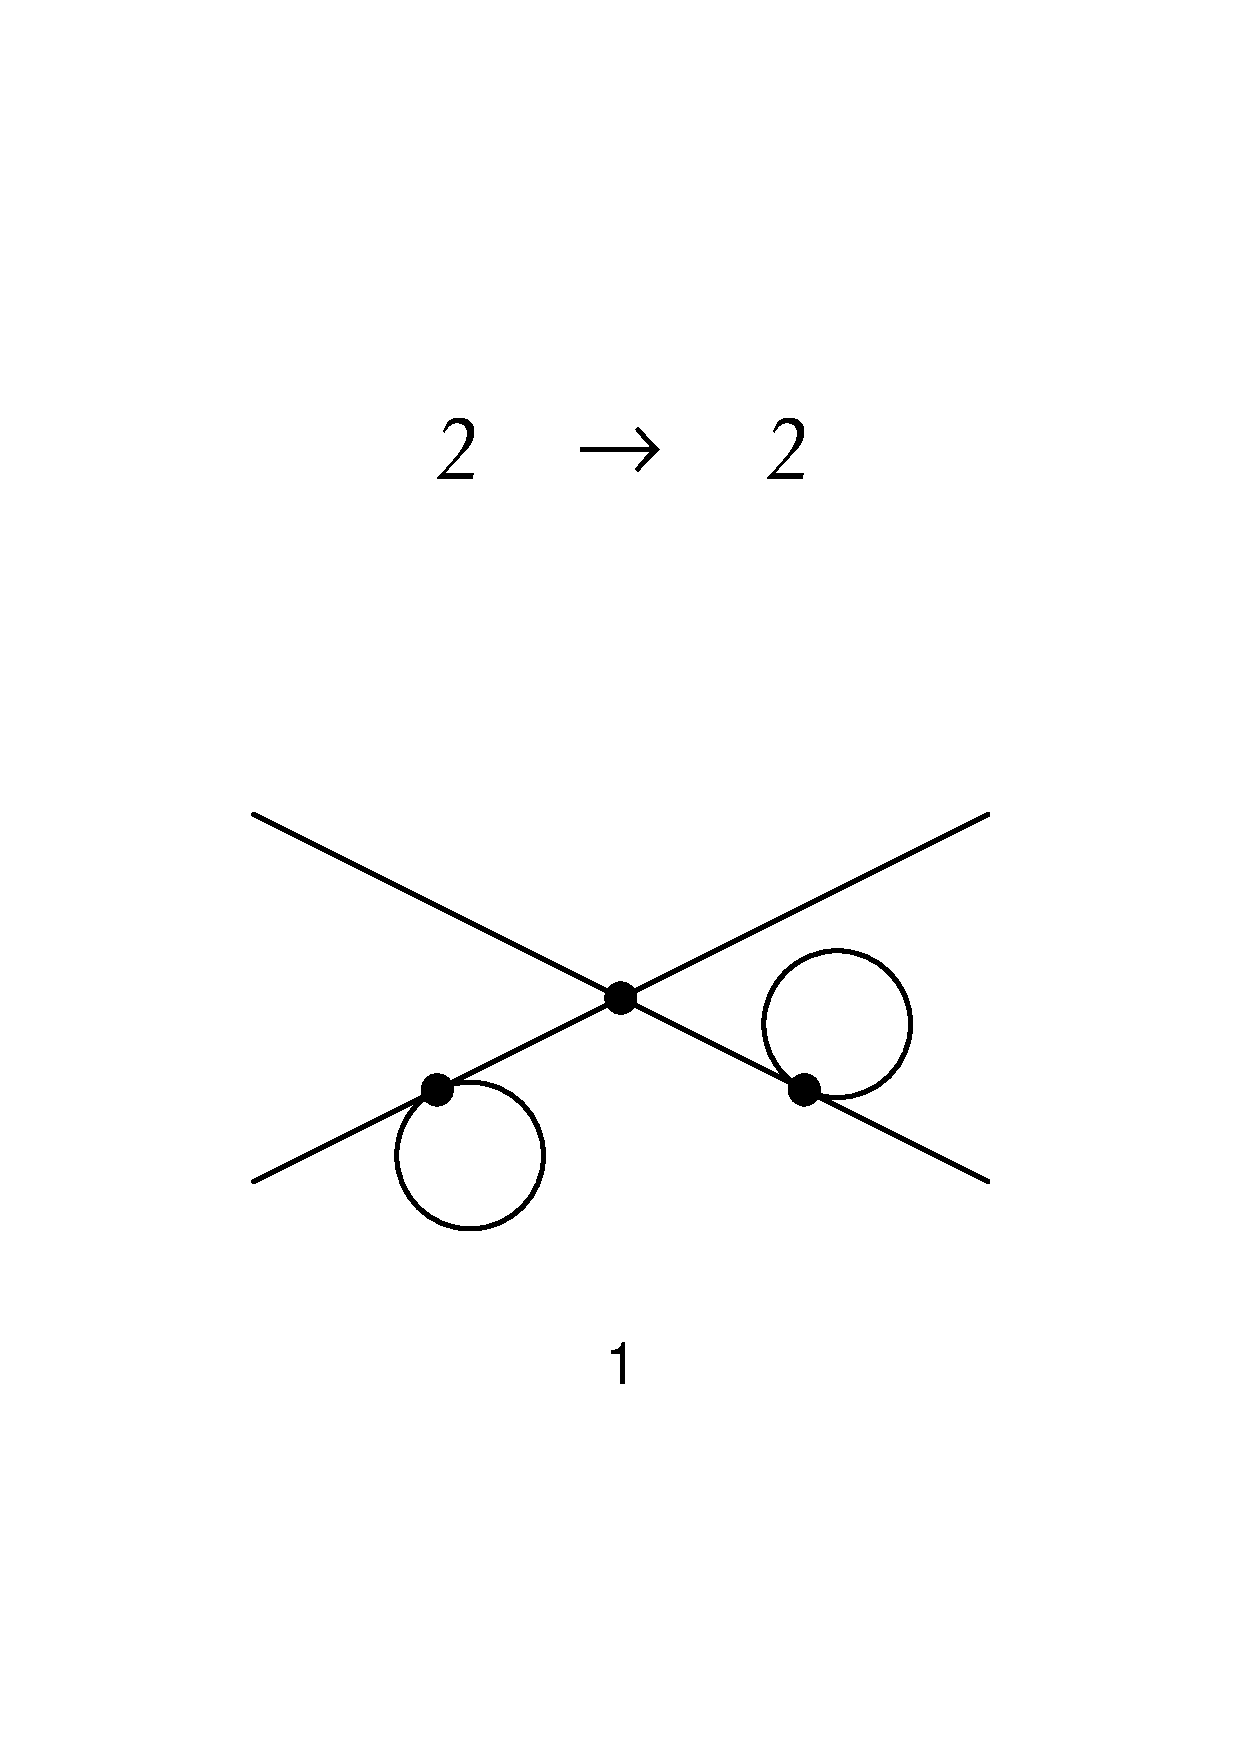
\includegraphics[width=0.28\textwidth]{generated/L2/images/topology25.pdf}
\end{center}
\noindent Parsed propagators: 8. Internal vertices: 3. Internal half-edges: 12.\\
\noindent Assignments checked: 32768. Surviving (nonzero vertex weight): 4096.\\
\noindent Raw $N_c$ power: 2. Net power in $C(t)$: -2.
\noindent Explicit surviving terms:
\begin{equation*}
\mathcal{T}_{25,1} = 64 i g_{2}^{3}\,N_c^{-2}\,G^<\left(x_1,z_{1}\right) \, G^<\left(z_{2},z_{1}\right) \, G_A\left(x_2,z_{2}\right) \, G_A\left(x_4,z_{3}\right) \, G_A\left(z_{2},z_{2}\right) \, G_A\left(z_{3},z_{1}\right) \, G_K\left(z_{3},z_{3}\right) \, G_R\left(x_3,z_{1}\right)
\end{equation*}
\begin{equation*}
\mathcal{T}_{25,2} = 64 i g_{2}^{3}\,N_c^{-2}\,G^<\left(x_1,z_{1}\right) \, G^<\left(z_{2},z_{1}\right) \, G_A\left(x_2,z_{2}\right) \, G_A\left(x_4,z_{3}\right) \, G_A\left(z_{2},z_{2}\right) \, G_A\left(z_{3},z_{3}\right) \, G_K\left(x_3,z_{1}\right) \, G_R\left(z_{3},z_{1}\right)
\end{equation*}
\begin{equation*}
\mathcal{T}_{25,3} = 64 i g_{2}^{3}\,N_c^{-2}\,G^<\left(x_1,z_{1}\right) \, G^<\left(z_{2},z_{1}\right) \, G_A\left(x_2,z_{2}\right) \, G_A\left(x_4,z_{3}\right) \, G_A\left(z_{2},z_{2}\right) \, G_A\left(z_{3},z_{3}\right) \, G_K\left(z_{3},z_{1}\right) \, G_R\left(x_3,z_{1}\right)
\end{equation*}
\begin{equation*}
\mathcal{T}_{25,4} = 64 i g_{2}^{3}\,N_c^{-2}\,G^<\left(x_1,z_{1}\right) \, G^<\left(z_{2},z_{1}\right) \, G_A\left(x_2,z_{2}\right) \, G_A\left(x_4,z_{3}\right) \, G_A\left(z_{2},z_{2}\right) \, G_K\left(x_3,z_{1}\right) \, G_R\left(z_{3},z_{1}\right) \, G_R\left(z_{3},z_{3}\right)
\end{equation*}
\begin{equation*}
\mathcal{T}_{25,5} = 64 i g_{2}^{3}\,N_c^{-2}\,G^<\left(x_1,z_{1}\right) \, G^<\left(z_{2},z_{1}\right) \, G_A\left(x_2,z_{2}\right) \, G_A\left(x_4,z_{3}\right) \, G_A\left(z_{2},z_{2}\right) \, G_K\left(z_{3},z_{1}\right) \, G_R\left(x_3,z_{1}\right) \, G_R\left(z_{3},z_{3}\right)
\end{equation*}
\begin{equation*}
\mathcal{T}_{25,6} = 64 i g_{2}^{3}\,N_c^{-2}\,G^<\left(x_1,z_{1}\right) \, G^<\left(z_{2},z_{1}\right) \, G_A\left(x_2,z_{2}\right) \, G_A\left(x_4,z_{3}\right) \, G_A\left(z_{3},z_{1}\right) \, G_K\left(z_{3},z_{3}\right) \, G_R\left(x_3,z_{1}\right) \, G_R\left(z_{2},z_{2}\right)
\end{equation*}
\begin{equation*}
\mathcal{T}_{25,7} = 64 i g_{2}^{3}\,N_c^{-2}\,G^<\left(x_1,z_{1}\right) \, G^<\left(z_{2},z_{1}\right) \, G_A\left(x_2,z_{2}\right) \, G_A\left(x_4,z_{3}\right) \, G_A\left(z_{3},z_{3}\right) \, G_K\left(x_3,z_{1}\right) \, G_R\left(z_{2},z_{2}\right) \, G_R\left(z_{3},z_{1}\right)
\end{equation*}
\begin{equation*}
\mathcal{T}_{25,8} = 64 i g_{2}^{3}\,N_c^{-2}\,G^<\left(x_1,z_{1}\right) \, G^<\left(z_{2},z_{1}\right) \, G_A\left(x_2,z_{2}\right) \, G_A\left(x_4,z_{3}\right) \, G_A\left(z_{3},z_{3}\right) \, G_K\left(z_{3},z_{1}\right) \, G_R\left(x_3,z_{1}\right) \, G_R\left(z_{2},z_{2}\right)
\end{equation*}
\begin{equation*}
\mathcal{T}_{25,9} = 64 i g_{2}^{3}\,N_c^{-2}\,G^<\left(x_1,z_{1}\right) \, G^<\left(z_{2},z_{1}\right) \, G_A\left(x_2,z_{2}\right) \, G_A\left(x_4,z_{3}\right) \, G_K\left(x_3,z_{1}\right) \, G_R\left(z_{2},z_{2}\right) \, G_R\left(z_{3},z_{1}\right) \, G_R\left(z_{3},z_{3}\right)
\end{equation*}
\begin{equation*}
\mathcal{T}_{25,10} = 64 i g_{2}^{3}\,N_c^{-2}\,G^<\left(x_1,z_{1}\right) \, G^<\left(z_{2},z_{1}\right) \, G_A\left(x_2,z_{2}\right) \, G_A\left(x_4,z_{3}\right) \, G_K\left(z_{3},z_{1}\right) \, G_R\left(x_3,z_{1}\right) \, G_R\left(z_{2},z_{2}\right) \, G_R\left(z_{3},z_{3}\right)
\end{equation*}
\begin{equation*}
\mathcal{T}_{25,11} = 64 i g_{2}^{3}\,N_c^{-2}\,G^>\left(x_3,z_{1}\right) \, G^>\left(z_{3},z_{1}\right) \, G_A\left(x_2,z_{2}\right) \, G_A\left(x_4,z_{3}\right) \, G_A\left(z_{2},z_{1}\right) \, G_A\left(z_{3},z_{3}\right) \, G_K\left(z_{2},z_{2}\right) \, G_R\left(x_1,z_{1}\right)
\end{equation*}
\begin{equation*}
\mathcal{T}_{25,12} = 64 i g_{2}^{3}\,N_c^{-2}\,G^>\left(x_3,z_{1}\right) \, G^>\left(z_{3},z_{1}\right) \, G_A\left(x_2,z_{2}\right) \, G_A\left(x_4,z_{3}\right) \, G_A\left(z_{2},z_{1}\right) \, G_K\left(z_{2},z_{2}\right) \, G_R\left(x_1,z_{1}\right) \, G_R\left(z_{3},z_{3}\right)
\end{equation*}
\begin{equation*}
\mathcal{T}_{25,13} = 64 i g_{2}^{3}\,N_c^{-2}\,G^>\left(x_3,z_{1}\right) \, G^>\left(z_{3},z_{1}\right) \, G_A\left(x_2,z_{2}\right) \, G_A\left(x_4,z_{3}\right) \, G_A\left(z_{2},z_{2}\right) \, G_A\left(z_{3},z_{3}\right) \, G_K\left(x_1,z_{1}\right) \, G_R\left(z_{2},z_{1}\right)
\end{equation*}
\begin{equation*}
\mathcal{T}_{25,14} = 64 i g_{2}^{3}\,N_c^{-2}\,G^>\left(x_3,z_{1}\right) \, G^>\left(z_{3},z_{1}\right) \, G_A\left(x_2,z_{2}\right) \, G_A\left(x_4,z_{3}\right) \, G_A\left(z_{2},z_{2}\right) \, G_A\left(z_{3},z_{3}\right) \, G_K\left(z_{2},z_{1}\right) \, G_R\left(x_1,z_{1}\right)
\end{equation*}
\begin{equation*}
\mathcal{T}_{25,15} = 64 i g_{2}^{3}\,N_c^{-2}\,G^>\left(x_3,z_{1}\right) \, G^>\left(z_{3},z_{1}\right) \, G_A\left(x_2,z_{2}\right) \, G_A\left(x_4,z_{3}\right) \, G_A\left(z_{2},z_{2}\right) \, G_K\left(x_1,z_{1}\right) \, G_R\left(z_{2},z_{1}\right) \, G_R\left(z_{3},z_{3}\right)
\end{equation*}
\begin{equation*}
\mathcal{T}_{25,16} = 64 i g_{2}^{3}\,N_c^{-2}\,G^>\left(x_3,z_{1}\right) \, G^>\left(z_{3},z_{1}\right) \, G_A\left(x_2,z_{2}\right) \, G_A\left(x_4,z_{3}\right) \, G_A\left(z_{2},z_{2}\right) \, G_K\left(z_{2},z_{1}\right) \, G_R\left(x_1,z_{1}\right) \, G_R\left(z_{3},z_{3}\right)
\end{equation*}
\begin{equation*}
\mathcal{T}_{25,17} = 64 i g_{2}^{3}\,N_c^{-2}\,G^>\left(x_3,z_{1}\right) \, G^>\left(z_{3},z_{1}\right) \, G_A\left(x_2,z_{2}\right) \, G_A\left(x_4,z_{3}\right) \, G_A\left(z_{3},z_{3}\right) \, G_K\left(x_1,z_{1}\right) \, G_R\left(z_{2},z_{1}\right) \, G_R\left(z_{2},z_{2}\right)
\end{equation*}
\begin{equation*}
\mathcal{T}_{25,18} = 64 i g_{2}^{3}\,N_c^{-2}\,G^>\left(x_3,z_{1}\right) \, G^>\left(z_{3},z_{1}\right) \, G_A\left(x_2,z_{2}\right) \, G_A\left(x_4,z_{3}\right) \, G_A\left(z_{3},z_{3}\right) \, G_K\left(z_{2},z_{1}\right) \, G_R\left(x_1,z_{1}\right) \, G_R\left(z_{2},z_{2}\right)
\end{equation*}
\begin{equation*}
\mathcal{T}_{25,19} = 64 i g_{2}^{3}\,N_c^{-2}\,G^>\left(x_3,z_{1}\right) \, G^>\left(z_{3},z_{1}\right) \, G_A\left(x_2,z_{2}\right) \, G_A\left(x_4,z_{3}\right) \, G_K\left(x_1,z_{1}\right) \, G_R\left(z_{2},z_{1}\right) \, G_R\left(z_{2},z_{2}\right) \, G_R\left(z_{3},z_{3}\right)
\end{equation*}
\begin{equation*}
\mathcal{T}_{25,20} = 64 i g_{2}^{3}\,N_c^{-2}\,G^>\left(x_3,z_{1}\right) \, G^>\left(z_{3},z_{1}\right) \, G_A\left(x_2,z_{2}\right) \, G_A\left(x_4,z_{3}\right) \, G_K\left(z_{2},z_{1}\right) \, G_R\left(x_1,z_{1}\right) \, G_R\left(z_{2},z_{2}\right) \, G_R\left(z_{3},z_{3}\right)
\end{equation*}
\section*{Topology 26 (FeynArts Topology 4)}
\begin{center}
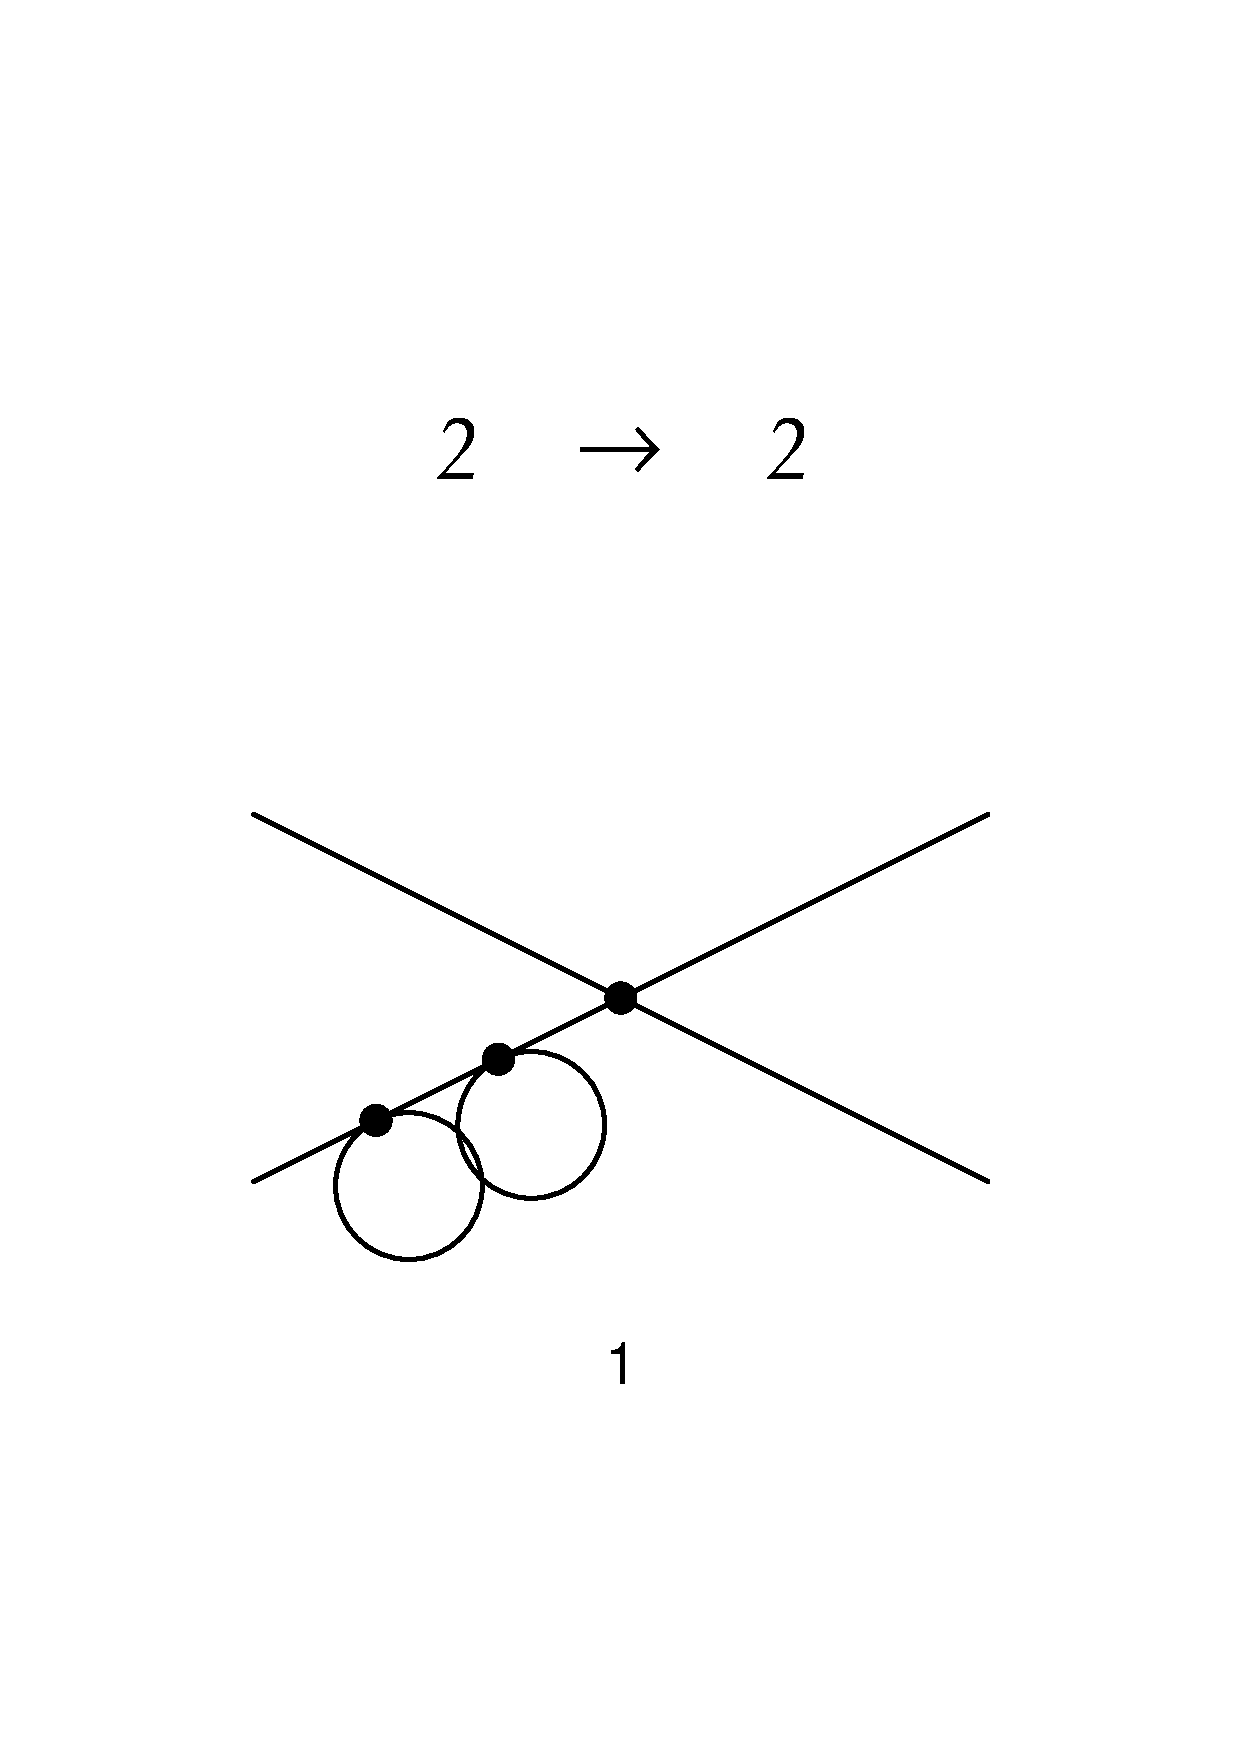
\includegraphics[width=0.28\textwidth]{generated/L2/images/topology26.pdf}
\end{center}
\noindent Parsed propagators: 8. Internal vertices: 3. Internal half-edges: 12.\\
\noindent Assignments checked: 32768. Surviving (nonzero vertex weight): 4096.\\
\noindent Raw $N_c$ power: 2. Net power in $C(t)$: -2.
\noindent Explicit surviving terms:
\begin{equation*}
\mathcal{T}_{26,1} = 64 i g_{2}^{3}\,N_c^{-2}\,G^<\left(x_1,z_{1}\right) \, G^<\left(z_{3},z_{1}\right) \, G_A\left(x_2,z_{2}\right) \, G_A\left(x_4,z_{1}\right) \, G_A\left(z_{2},z_{2}\right) \, G_A\left(z_{3},z_{2}\right) \, G_K\left(z_{3},z_{3}\right) \, G_R\left(x_3,z_{1}\right)
\end{equation*}
\begin{equation*}
\mathcal{T}_{26,2} = 64 i g_{2}^{3}\,N_c^{-2}\,G^<\left(x_1,z_{1}\right) \, G^<\left(z_{3},z_{1}\right) \, G_A\left(x_2,z_{2}\right) \, G_A\left(x_4,z_{1}\right) \, G_A\left(z_{2},z_{2}\right) \, G_A\left(z_{3},z_{3}\right) \, G_K\left(z_{3},z_{2}\right) \, G_R\left(x_3,z_{1}\right)
\end{equation*}
\begin{equation*}
\mathcal{T}_{26,3} = 64 i g_{2}^{3}\,N_c^{-2}\,G^<\left(x_1,z_{1}\right) \, G^<\left(z_{3},z_{1}\right) \, G_A\left(x_2,z_{2}\right) \, G_A\left(x_4,z_{1}\right) \, G_A\left(z_{2},z_{2}\right) \, G_K\left(z_{3},z_{2}\right) \, G_R\left(x_3,z_{1}\right) \, G_R\left(z_{3},z_{3}\right)
\end{equation*}
\begin{equation*}
\mathcal{T}_{26,4} = 64 i g_{2}^{3}\,N_c^{-2}\,G^<\left(x_1,z_{1}\right) \, G^<\left(z_{3},z_{1}\right) \, G_A\left(x_2,z_{2}\right) \, G_A\left(x_4,z_{1}\right) \, G_A\left(z_{3},z_{2}\right) \, G_K\left(z_{3},z_{3}\right) \, G_R\left(x_3,z_{1}\right) \, G_R\left(z_{2},z_{2}\right)
\end{equation*}
\begin{equation*}
\mathcal{T}_{26,5} = 64 i g_{2}^{3}\,N_c^{-2}\,G^<\left(x_1,z_{1}\right) \, G^<\left(z_{3},z_{1}\right) \, G_A\left(x_2,z_{2}\right) \, G_A\left(x_4,z_{1}\right) \, G_A\left(z_{3},z_{3}\right) \, G_K\left(z_{2},z_{2}\right) \, G_R\left(x_3,z_{1}\right) \, G_R\left(z_{3},z_{2}\right)
\end{equation*}
\begin{equation*}
\mathcal{T}_{26,6} = 64 i g_{2}^{3}\,N_c^{-2}\,G^<\left(x_1,z_{1}\right) \, G^<\left(z_{3},z_{1}\right) \, G_A\left(x_2,z_{2}\right) \, G_A\left(x_4,z_{1}\right) \, G_A\left(z_{3},z_{3}\right) \, G_K\left(z_{3},z_{2}\right) \, G_R\left(x_3,z_{1}\right) \, G_R\left(z_{2},z_{2}\right)
\end{equation*}
\begin{equation*}
\mathcal{T}_{26,7} = 64 i g_{2}^{3}\,N_c^{-2}\,G^<\left(x_1,z_{1}\right) \, G^<\left(z_{3},z_{1}\right) \, G_A\left(x_2,z_{2}\right) \, G_A\left(x_4,z_{1}\right) \, G_K\left(z_{2},z_{2}\right) \, G_R\left(x_3,z_{1}\right) \, G_R\left(z_{3},z_{2}\right) \, G_R\left(z_{3},z_{3}\right)
\end{equation*}
\begin{equation*}
\mathcal{T}_{26,8} = 64 i g_{2}^{3}\,N_c^{-2}\,G^<\left(x_1,z_{1}\right) \, G^<\left(z_{3},z_{1}\right) \, G_A\left(x_2,z_{2}\right) \, G_A\left(x_4,z_{1}\right) \, G_K\left(z_{3},z_{2}\right) \, G_R\left(x_3,z_{1}\right) \, G_R\left(z_{2},z_{2}\right) \, G_R\left(z_{3},z_{3}\right)
\end{equation*}
\begin{equation*}
\mathcal{T}_{26,9} = 64 i g_{2}^{3}\,N_c^{-2}\,G^<\left(x_1,z_{1}\right) \, G^>\left(z_{3},z_{2}\right) \, G_A\left(x_2,z_{2}\right) \, G_A\left(x_4,z_{1}\right) \, G_A\left(z_{2},z_{2}\right) \, G_A\left(z_{3},z_{1}\right) \, G_K\left(z_{3},z_{3}\right) \, G_R\left(x_3,z_{1}\right)
\end{equation*}
\begin{equation*}
\mathcal{T}_{26,10} = 64 i g_{2}^{3}\,N_c^{-2}\,G^<\left(x_1,z_{1}\right) \, G^>\left(z_{3},z_{2}\right) \, G_A\left(x_2,z_{2}\right) \, G_A\left(x_4,z_{1}\right) \, G_A\left(z_{2},z_{2}\right) \, G_A\left(z_{3},z_{3}\right) \, G_K\left(x_3,z_{1}\right) \, G_R\left(z_{3},z_{1}\right)
\end{equation*}
\begin{equation*}
\mathcal{T}_{26,11} = 64 i g_{2}^{3}\,N_c^{-2}\,G^<\left(x_1,z_{1}\right) \, G^>\left(z_{3},z_{2}\right) \, G_A\left(x_2,z_{2}\right) \, G_A\left(x_4,z_{1}\right) \, G_A\left(z_{2},z_{2}\right) \, G_A\left(z_{3},z_{3}\right) \, G_K\left(z_{3},z_{1}\right) \, G_R\left(x_3,z_{1}\right)
\end{equation*}
\begin{equation*}
\mathcal{T}_{26,12} = 64 i g_{2}^{3}\,N_c^{-2}\,G^<\left(x_1,z_{1}\right) \, G^>\left(z_{3},z_{2}\right) \, G_A\left(x_2,z_{2}\right) \, G_A\left(x_4,z_{1}\right) \, G_A\left(z_{2},z_{2}\right) \, G_K\left(x_3,z_{1}\right) \, G_R\left(z_{3},z_{1}\right) \, G_R\left(z_{3},z_{3}\right)
\end{equation*}
\begin{equation*}
\mathcal{T}_{26,13} = 64 i g_{2}^{3}\,N_c^{-2}\,G^<\left(x_1,z_{1}\right) \, G^>\left(z_{3},z_{2}\right) \, G_A\left(x_2,z_{2}\right) \, G_A\left(x_4,z_{1}\right) \, G_A\left(z_{2},z_{2}\right) \, G_K\left(z_{3},z_{1}\right) \, G_R\left(x_3,z_{1}\right) \, G_R\left(z_{3},z_{3}\right)
\end{equation*}
\begin{equation*}
\mathcal{T}_{26,14} = 64 i g_{2}^{3}\,N_c^{-2}\,G^<\left(x_1,z_{1}\right) \, G^>\left(z_{3},z_{2}\right) \, G_A\left(x_2,z_{2}\right) \, G_A\left(x_4,z_{1}\right) \, G_A\left(z_{3},z_{1}\right) \, G_K\left(z_{3},z_{3}\right) \, G_R\left(x_3,z_{1}\right) \, G_R\left(z_{2},z_{2}\right)
\end{equation*}
\begin{equation*}
\mathcal{T}_{26,15} = 64 i g_{2}^{3}\,N_c^{-2}\,G^<\left(x_1,z_{1}\right) \, G^>\left(z_{3},z_{2}\right) \, G_A\left(x_2,z_{2}\right) \, G_A\left(x_4,z_{1}\right) \, G_A\left(z_{3},z_{3}\right) \, G_K\left(x_3,z_{1}\right) \, G_R\left(z_{2},z_{2}\right) \, G_R\left(z_{3},z_{1}\right)
\end{equation*}
\begin{equation*}
\mathcal{T}_{26,16} = 64 i g_{2}^{3}\,N_c^{-2}\,G^<\left(x_1,z_{1}\right) \, G^>\left(z_{3},z_{2}\right) \, G_A\left(x_2,z_{2}\right) \, G_A\left(x_4,z_{1}\right) \, G_A\left(z_{3},z_{3}\right) \, G_K\left(z_{3},z_{1}\right) \, G_R\left(x_3,z_{1}\right) \, G_R\left(z_{2},z_{2}\right)
\end{equation*}
\begin{equation*}
\mathcal{T}_{26,17} = 64 i g_{2}^{3}\,N_c^{-2}\,G^<\left(x_1,z_{1}\right) \, G^>\left(z_{3},z_{2}\right) \, G_A\left(x_2,z_{2}\right) \, G_A\left(x_4,z_{1}\right) \, G_K\left(x_3,z_{1}\right) \, G_R\left(z_{2},z_{2}\right) \, G_R\left(z_{3},z_{1}\right) \, G_R\left(z_{3},z_{3}\right)
\end{equation*}
\begin{equation*}
\mathcal{T}_{26,18} = 64 i g_{2}^{3}\,N_c^{-2}\,G^<\left(x_1,z_{1}\right) \, G^>\left(z_{3},z_{2}\right) \, G_A\left(x_2,z_{2}\right) \, G_A\left(x_4,z_{1}\right) \, G_K\left(z_{3},z_{1}\right) \, G_R\left(x_3,z_{1}\right) \, G_R\left(z_{2},z_{2}\right) \, G_R\left(z_{3},z_{3}\right)
\end{equation*}
\section*{Topology 27 (FeynArts Topology 4)}
\begin{center}
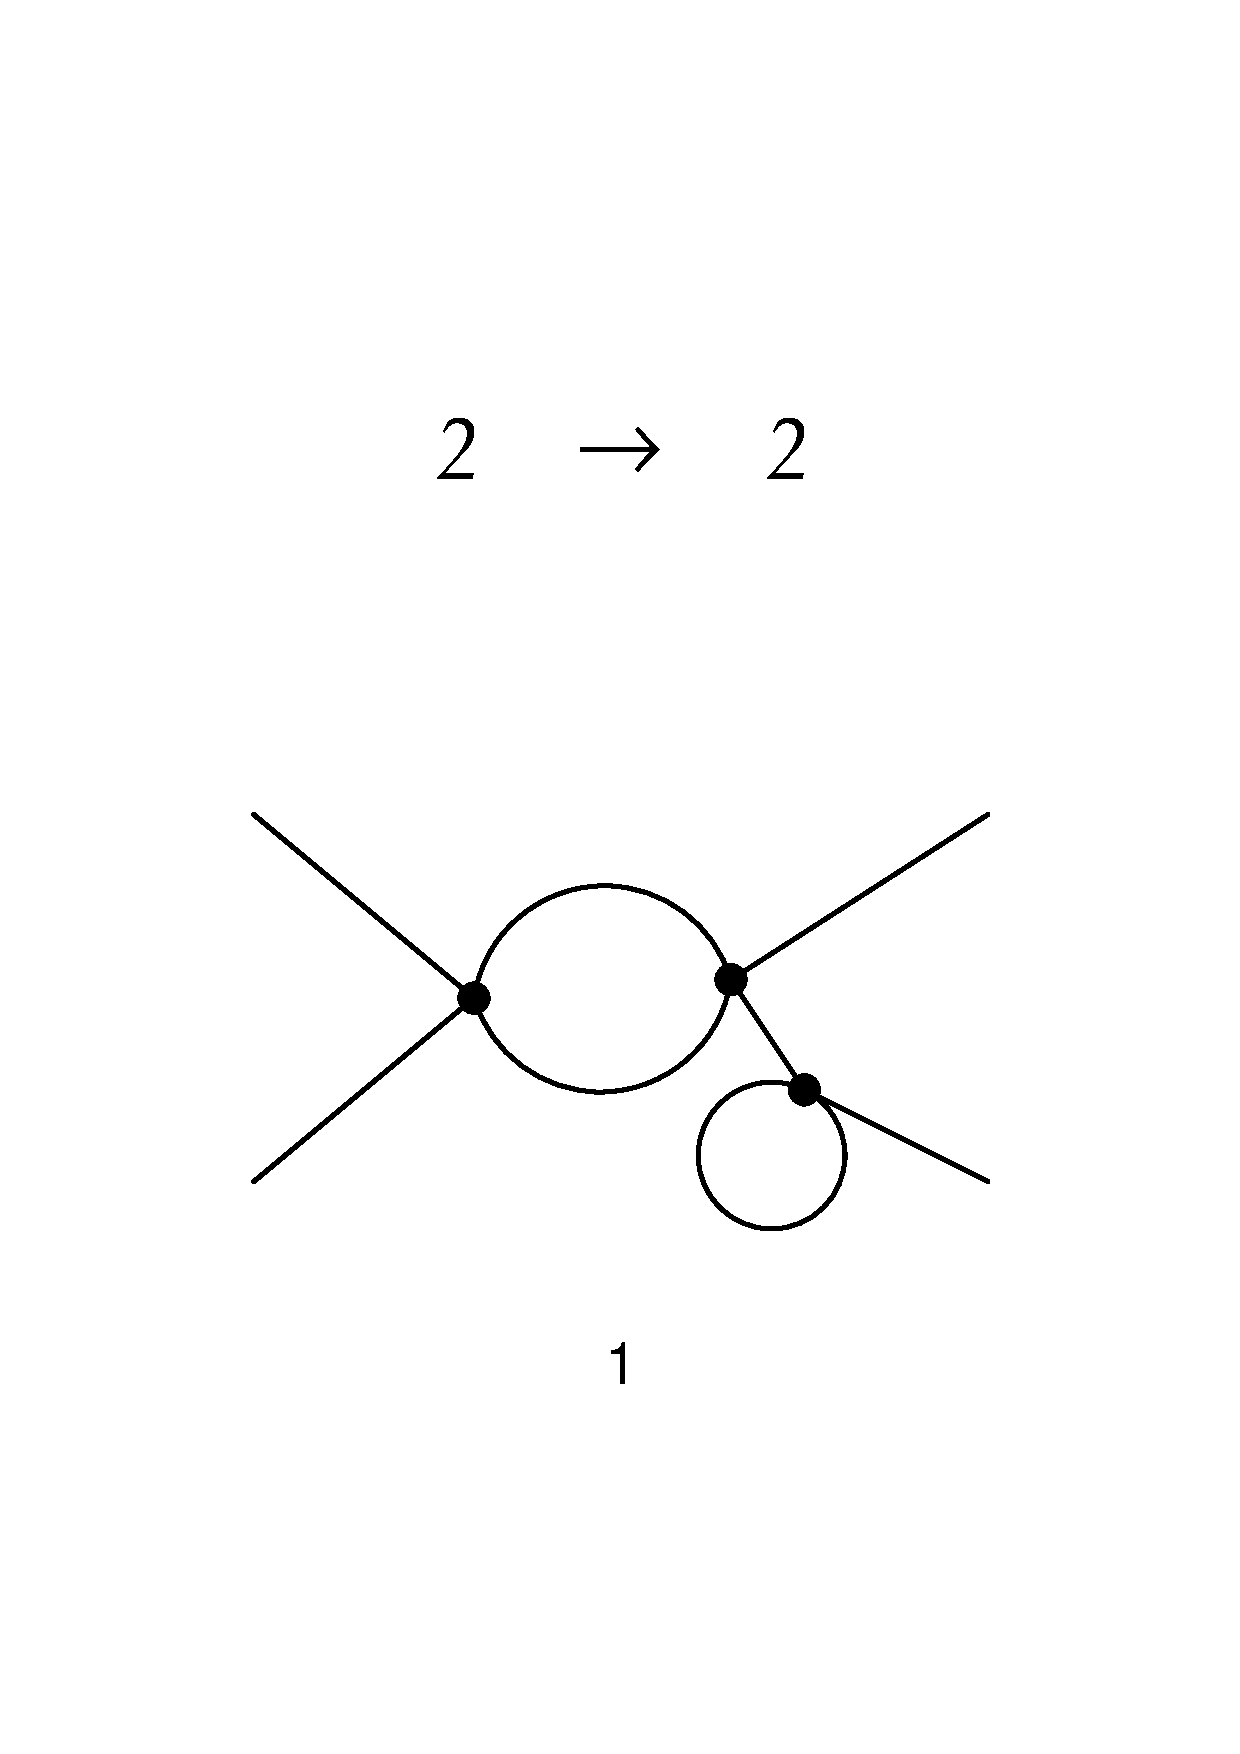
\includegraphics[width=0.28\textwidth]{generated/L2/images/topology27.pdf}
\end{center}
\noindent Parsed propagators: 8. Internal vertices: 3. Internal half-edges: 12.\\
\noindent Assignments checked: 32768. Surviving (nonzero vertex weight): 4096.\\
\noindent Raw $N_c$ power: 1. Net power in $C(t)$: -3.
\noindent Explicit surviving terms:
\begin{equation*}
\mathcal{T}_{27,1} = 128 i g_{2}^{3}\,N_c^{-3}\,G^>\left(x_3,z_{2}\right) \, G^>\left(z_{3},z_{2}\right) \, G_A\left(x_2,z_{1}\right) \, G_A\left(x_4,z_{3}\right) \, G_A\left(z_{2},z_{1}\right) \, G_A\left(z_{3},z_{3}\right) \, G_K\left(x_1,z_{1}\right) \, G_R\left(z_{2},z_{1}\right)
\end{equation*}
\begin{equation*}
\mathcal{T}_{27,2} = 128 i g_{2}^{3}\,N_c^{-3}\,G^>\left(x_3,z_{2}\right) \, G^>\left(z_{3},z_{2}\right) \, G_A\left(x_2,z_{1}\right) \, G_A\left(x_4,z_{3}\right) \, G_A\left(z_{2},z_{1}\right) \, G_A\left(z_{3},z_{3}\right) \, G_K\left(z_{2},z_{1}\right) \, G_R\left(x_1,z_{1}\right)
\end{equation*}
\begin{equation*}
\mathcal{T}_{27,3} = 128 i g_{2}^{3}\,N_c^{-3}\,G^>\left(x_3,z_{2}\right) \, G^>\left(z_{3},z_{2}\right) \, G_A\left(x_2,z_{1}\right) \, G_A\left(x_4,z_{3}\right) \, G_A\left(z_{2},z_{1}\right) \, G_K\left(x_1,z_{1}\right) \, G_R\left(z_{2},z_{1}\right) \, G_R\left(z_{3},z_{3}\right)
\end{equation*}
\begin{equation*}
\mathcal{T}_{27,4} = 128 i g_{2}^{3}\,N_c^{-3}\,G^>\left(x_3,z_{2}\right) \, G^>\left(z_{3},z_{2}\right) \, G_A\left(x_2,z_{1}\right) \, G_A\left(x_4,z_{3}\right) \, G_A\left(z_{2},z_{1}\right) \, G_K\left(z_{2},z_{1}\right) \, G_R\left(x_1,z_{1}\right) \, G_R\left(z_{3},z_{3}\right)
\end{equation*}
\begin{equation*}
\mathcal{T}_{27,5} = 64 i g_{2}^{3}\,N_c^{-3}\,G^>\left(z_{2},z_{1}\right) \, G^>\left(z_{2},z_{1}\right) \, G_A\left(x_2,z_{1}\right) \, G_A\left(x_4,z_{3}\right) \, G_A\left(z_{3},z_{2}\right) \, G_K\left(z_{3},z_{3}\right) \, G_R\left(x_1,z_{1}\right) \, G_R\left(x_3,z_{2}\right)
\end{equation*}
\begin{equation*}
\mathcal{T}_{27,6} = 64 i g_{2}^{3}\,N_c^{-3}\,G^>\left(z_{2},z_{1}\right) \, G^>\left(z_{2},z_{1}\right) \, G_A\left(x_2,z_{1}\right) \, G_A\left(x_4,z_{3}\right) \, G_A\left(z_{3},z_{3}\right) \, G_K\left(x_3,z_{2}\right) \, G_R\left(x_1,z_{1}\right) \, G_R\left(z_{3},z_{2}\right)
\end{equation*}
\begin{equation*}
\mathcal{T}_{27,7} = 64 i g_{2}^{3}\,N_c^{-3}\,G^>\left(z_{2},z_{1}\right) \, G^>\left(z_{2},z_{1}\right) \, G_A\left(x_2,z_{1}\right) \, G_A\left(x_4,z_{3}\right) \, G_A\left(z_{3},z_{3}\right) \, G_K\left(z_{3},z_{2}\right) \, G_R\left(x_1,z_{1}\right) \, G_R\left(x_3,z_{2}\right)
\end{equation*}
\begin{equation*}
\mathcal{T}_{27,8} = 64 i g_{2}^{3}\,N_c^{-3}\,G^>\left(z_{2},z_{1}\right) \, G^>\left(z_{2},z_{1}\right) \, G_A\left(x_2,z_{1}\right) \, G_A\left(x_4,z_{3}\right) \, G_K\left(x_3,z_{2}\right) \, G_R\left(x_1,z_{1}\right) \, G_R\left(z_{3},z_{2}\right) \, G_R\left(z_{3},z_{3}\right)
\end{equation*}
\begin{equation*}
\mathcal{T}_{27,9} = 64 i g_{2}^{3}\,N_c^{-3}\,G^>\left(z_{2},z_{1}\right) \, G^>\left(z_{2},z_{1}\right) \, G_A\left(x_2,z_{1}\right) \, G_A\left(x_4,z_{3}\right) \, G_K\left(z_{3},z_{2}\right) \, G_R\left(x_1,z_{1}\right) \, G_R\left(x_3,z_{2}\right) \, G_R\left(z_{3},z_{3}\right)
\end{equation*}
\section*{Topology 28 (FeynArts Topology 4)}
\begin{center}
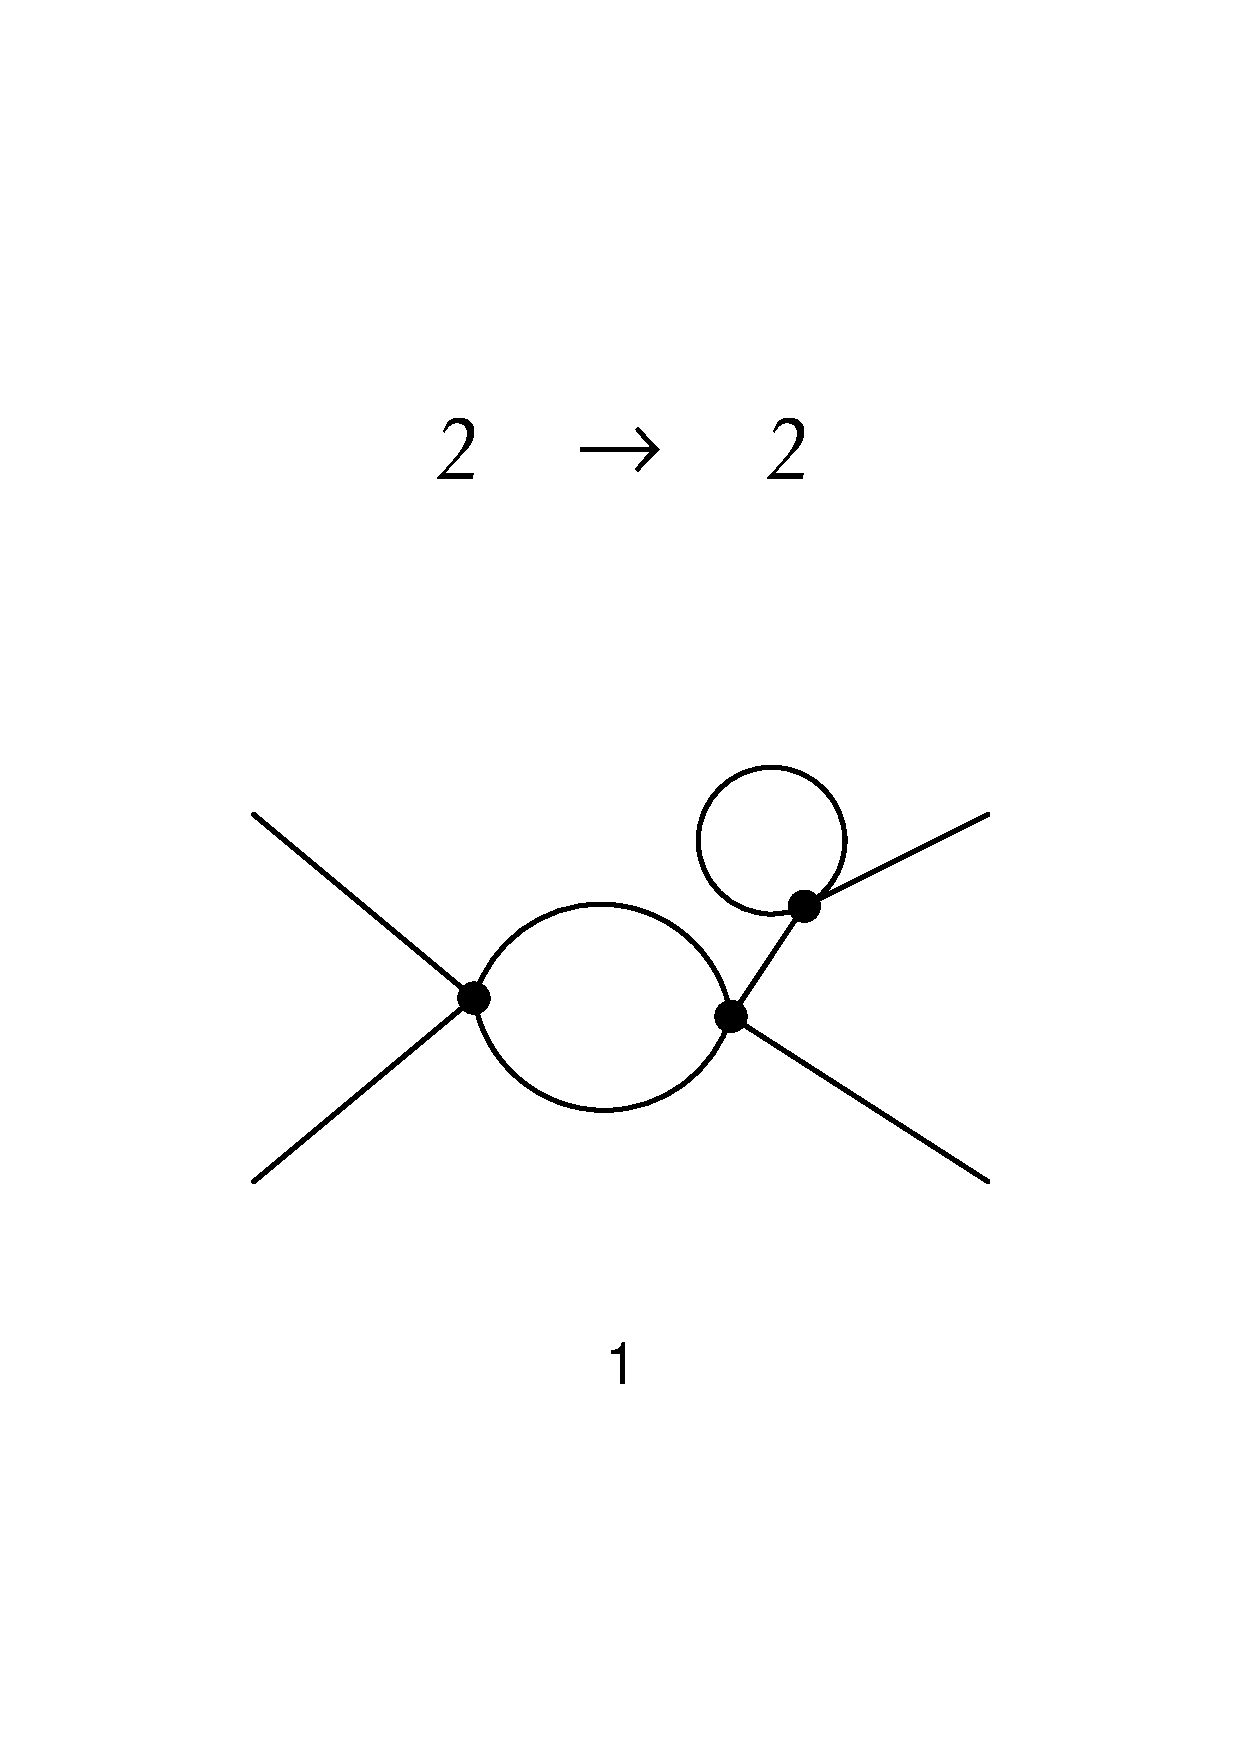
\includegraphics[width=0.28\textwidth]{generated/L2/images/topology28.pdf}
\end{center}
\noindent Parsed propagators: 8. Internal vertices: 3. Internal half-edges: 12.\\
\noindent Assignments checked: 32768. Surviving (nonzero vertex weight): 4096.\\
\noindent Raw $N_c$ power: 1. Net power in $C(t)$: -3.
\noindent Explicit surviving terms:
\begin{equation*}
\mathcal{T}_{28,1} = 64 i g_{2}^{3}\,N_c^{-3}\,G^>\left(z_{3},z_{1}\right) \, G^>\left(z_{3},z_{1}\right) \, G_A\left(x_2,z_{1}\right) \, G_A\left(x_4,z_{3}\right) \, G_A\left(z_{2},z_{2}\right) \, G_A\left(z_{3},z_{2}\right) \, G_K\left(x_3,z_{2}\right) \, G_R\left(x_1,z_{1}\right)
\end{equation*}
\begin{equation*}
\mathcal{T}_{28,2} = 64 i g_{2}^{3}\,N_c^{-3}\,G^>\left(z_{3},z_{1}\right) \, G^>\left(z_{3},z_{1}\right) \, G_A\left(x_2,z_{1}\right) \, G_A\left(x_4,z_{3}\right) \, G_A\left(z_{3},z_{2}\right) \, G_K\left(x_3,z_{2}\right) \, G_R\left(x_1,z_{1}\right) \, G_R\left(z_{2},z_{2}\right)
\end{equation*}
\begin{equation*}
\mathcal{T}_{28,3} = 64 i g_{2}^{3}\,N_c^{-3}\,G^>\left(z_{3},z_{1}\right) \, G^>\left(z_{3},z_{1}\right) \, G_A\left(x_2,z_{1}\right) \, G_A\left(x_4,z_{3}\right) \, G_A\left(z_{3},z_{2}\right) \, G_K\left(z_{2},z_{2}\right) \, G_R\left(x_1,z_{1}\right) \, G_R\left(x_3,z_{2}\right)
\end{equation*}
\section*{Topology 29 (FeynArts Topology 4)}
\begin{center}
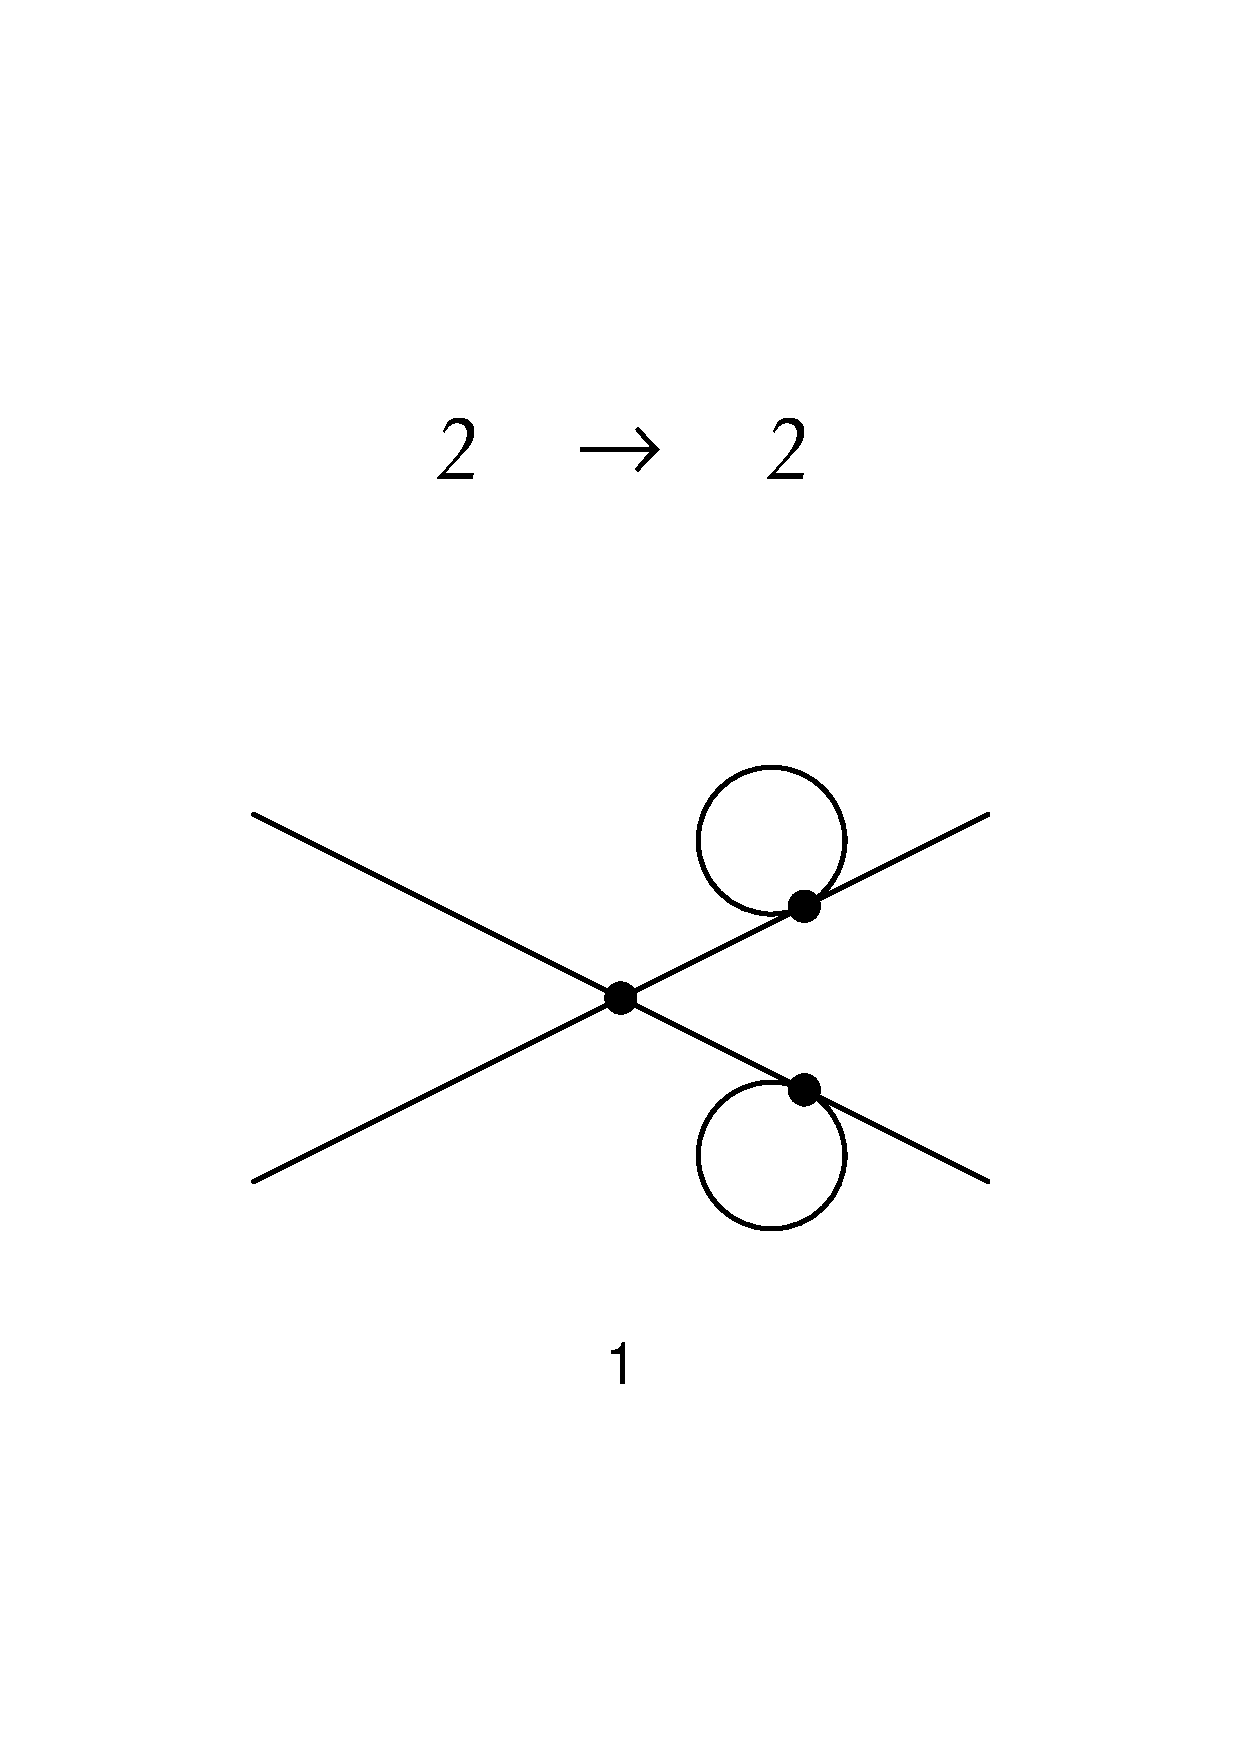
\includegraphics[width=0.28\textwidth]{generated/L2/images/topology29.pdf}
\end{center}
\noindent Parsed propagators: 8. Internal vertices: 3. Internal half-edges: 12.\\
\noindent Assignments checked: 32768. Surviving (nonzero vertex weight): 4096.\\
\noindent Raw $N_c$ power: 2. Net power in $C(t)$: -2.
\noindent Explicit surviving terms:
\begin{equation*}
\mathcal{T}_{29,1} = 64 i g_{2}^{3}\,N_c^{-2}\,G^>\left(x_3,z_{2}\right) \, G^>\left(z_{3},z_{1}\right) \, G_A\left(x_2,z_{1}\right) \, G_A\left(x_4,z_{3}\right) \, G_A\left(z_{2},z_{1}\right) \, G_A\left(z_{3},z_{3}\right) \, G_K\left(z_{2},z_{2}\right) \, G_R\left(x_1,z_{1}\right)
\end{equation*}
\begin{equation*}
\mathcal{T}_{29,2} = 64 i g_{2}^{3}\,N_c^{-2}\,G^>\left(x_3,z_{2}\right) \, G^>\left(z_{3},z_{1}\right) \, G_A\left(x_2,z_{1}\right) \, G_A\left(x_4,z_{3}\right) \, G_A\left(z_{2},z_{1}\right) \, G_K\left(z_{2},z_{2}\right) \, G_R\left(x_1,z_{1}\right) \, G_R\left(z_{3},z_{3}\right)
\end{equation*}
\begin{equation*}
\mathcal{T}_{29,3} = 64 i g_{2}^{3}\,N_c^{-2}\,G^>\left(x_3,z_{2}\right) \, G^>\left(z_{3},z_{1}\right) \, G_A\left(x_2,z_{1}\right) \, G_A\left(x_4,z_{3}\right) \, G_A\left(z_{2},z_{2}\right) \, G_A\left(z_{3},z_{3}\right) \, G_K\left(x_1,z_{1}\right) \, G_R\left(z_{2},z_{1}\right)
\end{equation*}
\begin{equation*}
\mathcal{T}_{29,4} = 64 i g_{2}^{3}\,N_c^{-2}\,G^>\left(x_3,z_{2}\right) \, G^>\left(z_{3},z_{1}\right) \, G_A\left(x_2,z_{1}\right) \, G_A\left(x_4,z_{3}\right) \, G_A\left(z_{2},z_{2}\right) \, G_A\left(z_{3},z_{3}\right) \, G_K\left(z_{2},z_{1}\right) \, G_R\left(x_1,z_{1}\right)
\end{equation*}
\begin{equation*}
\mathcal{T}_{29,5} = 64 i g_{2}^{3}\,N_c^{-2}\,G^>\left(x_3,z_{2}\right) \, G^>\left(z_{3},z_{1}\right) \, G_A\left(x_2,z_{1}\right) \, G_A\left(x_4,z_{3}\right) \, G_A\left(z_{2},z_{2}\right) \, G_K\left(x_1,z_{1}\right) \, G_R\left(z_{2},z_{1}\right) \, G_R\left(z_{3},z_{3}\right)
\end{equation*}
\begin{equation*}
\mathcal{T}_{29,6} = 64 i g_{2}^{3}\,N_c^{-2}\,G^>\left(x_3,z_{2}\right) \, G^>\left(z_{3},z_{1}\right) \, G_A\left(x_2,z_{1}\right) \, G_A\left(x_4,z_{3}\right) \, G_A\left(z_{2},z_{2}\right) \, G_K\left(z_{2},z_{1}\right) \, G_R\left(x_1,z_{1}\right) \, G_R\left(z_{3},z_{3}\right)
\end{equation*}
\begin{equation*}
\mathcal{T}_{29,7} = 64 i g_{2}^{3}\,N_c^{-2}\,G^>\left(x_3,z_{2}\right) \, G^>\left(z_{3},z_{1}\right) \, G_A\left(x_2,z_{1}\right) \, G_A\left(x_4,z_{3}\right) \, G_A\left(z_{3},z_{3}\right) \, G_K\left(x_1,z_{1}\right) \, G_R\left(z_{2},z_{1}\right) \, G_R\left(z_{2},z_{2}\right)
\end{equation*}
\begin{equation*}
\mathcal{T}_{29,8} = 64 i g_{2}^{3}\,N_c^{-2}\,G^>\left(x_3,z_{2}\right) \, G^>\left(z_{3},z_{1}\right) \, G_A\left(x_2,z_{1}\right) \, G_A\left(x_4,z_{3}\right) \, G_A\left(z_{3},z_{3}\right) \, G_K\left(z_{2},z_{1}\right) \, G_R\left(x_1,z_{1}\right) \, G_R\left(z_{2},z_{2}\right)
\end{equation*}
\begin{equation*}
\mathcal{T}_{29,9} = 64 i g_{2}^{3}\,N_c^{-2}\,G^>\left(x_3,z_{2}\right) \, G^>\left(z_{3},z_{1}\right) \, G_A\left(x_2,z_{1}\right) \, G_A\left(x_4,z_{3}\right) \, G_K\left(x_1,z_{1}\right) \, G_R\left(z_{2},z_{1}\right) \, G_R\left(z_{2},z_{2}\right) \, G_R\left(z_{3},z_{3}\right)
\end{equation*}
\begin{equation*}
\mathcal{T}_{29,10} = 64 i g_{2}^{3}\,N_c^{-2}\,G^>\left(x_3,z_{2}\right) \, G^>\left(z_{3},z_{1}\right) \, G_A\left(x_2,z_{1}\right) \, G_A\left(x_4,z_{3}\right) \, G_K\left(z_{2},z_{1}\right) \, G_R\left(x_1,z_{1}\right) \, G_R\left(z_{2},z_{2}\right) \, G_R\left(z_{3},z_{3}\right)
\end{equation*}
\begin{equation*}
\mathcal{T}_{29,11} = 64 i g_{2}^{3}\,N_c^{-2}\,G^>\left(z_{2},z_{1}\right) \, G^>\left(z_{3},z_{1}\right) \, G_A\left(x_2,z_{1}\right) \, G_A\left(x_4,z_{3}\right) \, G_A\left(z_{2},z_{2}\right) \, G_A\left(z_{3},z_{3}\right) \, G_K\left(x_3,z_{2}\right) \, G_R\left(x_1,z_{1}\right)
\end{equation*}
\begin{equation*}
\mathcal{T}_{29,12} = 64 i g_{2}^{3}\,N_c^{-2}\,G^>\left(z_{2},z_{1}\right) \, G^>\left(z_{3},z_{1}\right) \, G_A\left(x_2,z_{1}\right) \, G_A\left(x_4,z_{3}\right) \, G_A\left(z_{2},z_{2}\right) \, G_K\left(x_3,z_{2}\right) \, G_R\left(x_1,z_{1}\right) \, G_R\left(z_{3},z_{3}\right)
\end{equation*}
\begin{equation*}
\mathcal{T}_{29,13} = 64 i g_{2}^{3}\,N_c^{-2}\,G^>\left(z_{2},z_{1}\right) \, G^>\left(z_{3},z_{1}\right) \, G_A\left(x_2,z_{1}\right) \, G_A\left(x_4,z_{3}\right) \, G_A\left(z_{3},z_{3}\right) \, G_K\left(x_3,z_{2}\right) \, G_R\left(x_1,z_{1}\right) \, G_R\left(z_{2},z_{2}\right)
\end{equation*}
\begin{equation*}
\mathcal{T}_{29,14} = 64 i g_{2}^{3}\,N_c^{-2}\,G^>\left(z_{2},z_{1}\right) \, G^>\left(z_{3},z_{1}\right) \, G_A\left(x_2,z_{1}\right) \, G_A\left(x_4,z_{3}\right) \, G_A\left(z_{3},z_{3}\right) \, G_K\left(z_{2},z_{2}\right) \, G_R\left(x_1,z_{1}\right) \, G_R\left(x_3,z_{2}\right)
\end{equation*}
\begin{equation*}
\mathcal{T}_{29,15} = 64 i g_{2}^{3}\,N_c^{-2}\,G^>\left(z_{2},z_{1}\right) \, G^>\left(z_{3},z_{1}\right) \, G_A\left(x_2,z_{1}\right) \, G_A\left(x_4,z_{3}\right) \, G_K\left(x_3,z_{2}\right) \, G_R\left(x_1,z_{1}\right) \, G_R\left(z_{2},z_{2}\right) \, G_R\left(z_{3},z_{3}\right)
\end{equation*}
\begin{equation*}
\mathcal{T}_{29,16} = 64 i g_{2}^{3}\,N_c^{-2}\,G^>\left(z_{2},z_{1}\right) \, G^>\left(z_{3},z_{1}\right) \, G_A\left(x_2,z_{1}\right) \, G_A\left(x_4,z_{3}\right) \, G_K\left(z_{2},z_{2}\right) \, G_R\left(x_1,z_{1}\right) \, G_R\left(x_3,z_{2}\right) \, G_R\left(z_{3},z_{3}\right)
\end{equation*}
\section*{Topology 30 (FeynArts Topology 4)}
\begin{center}
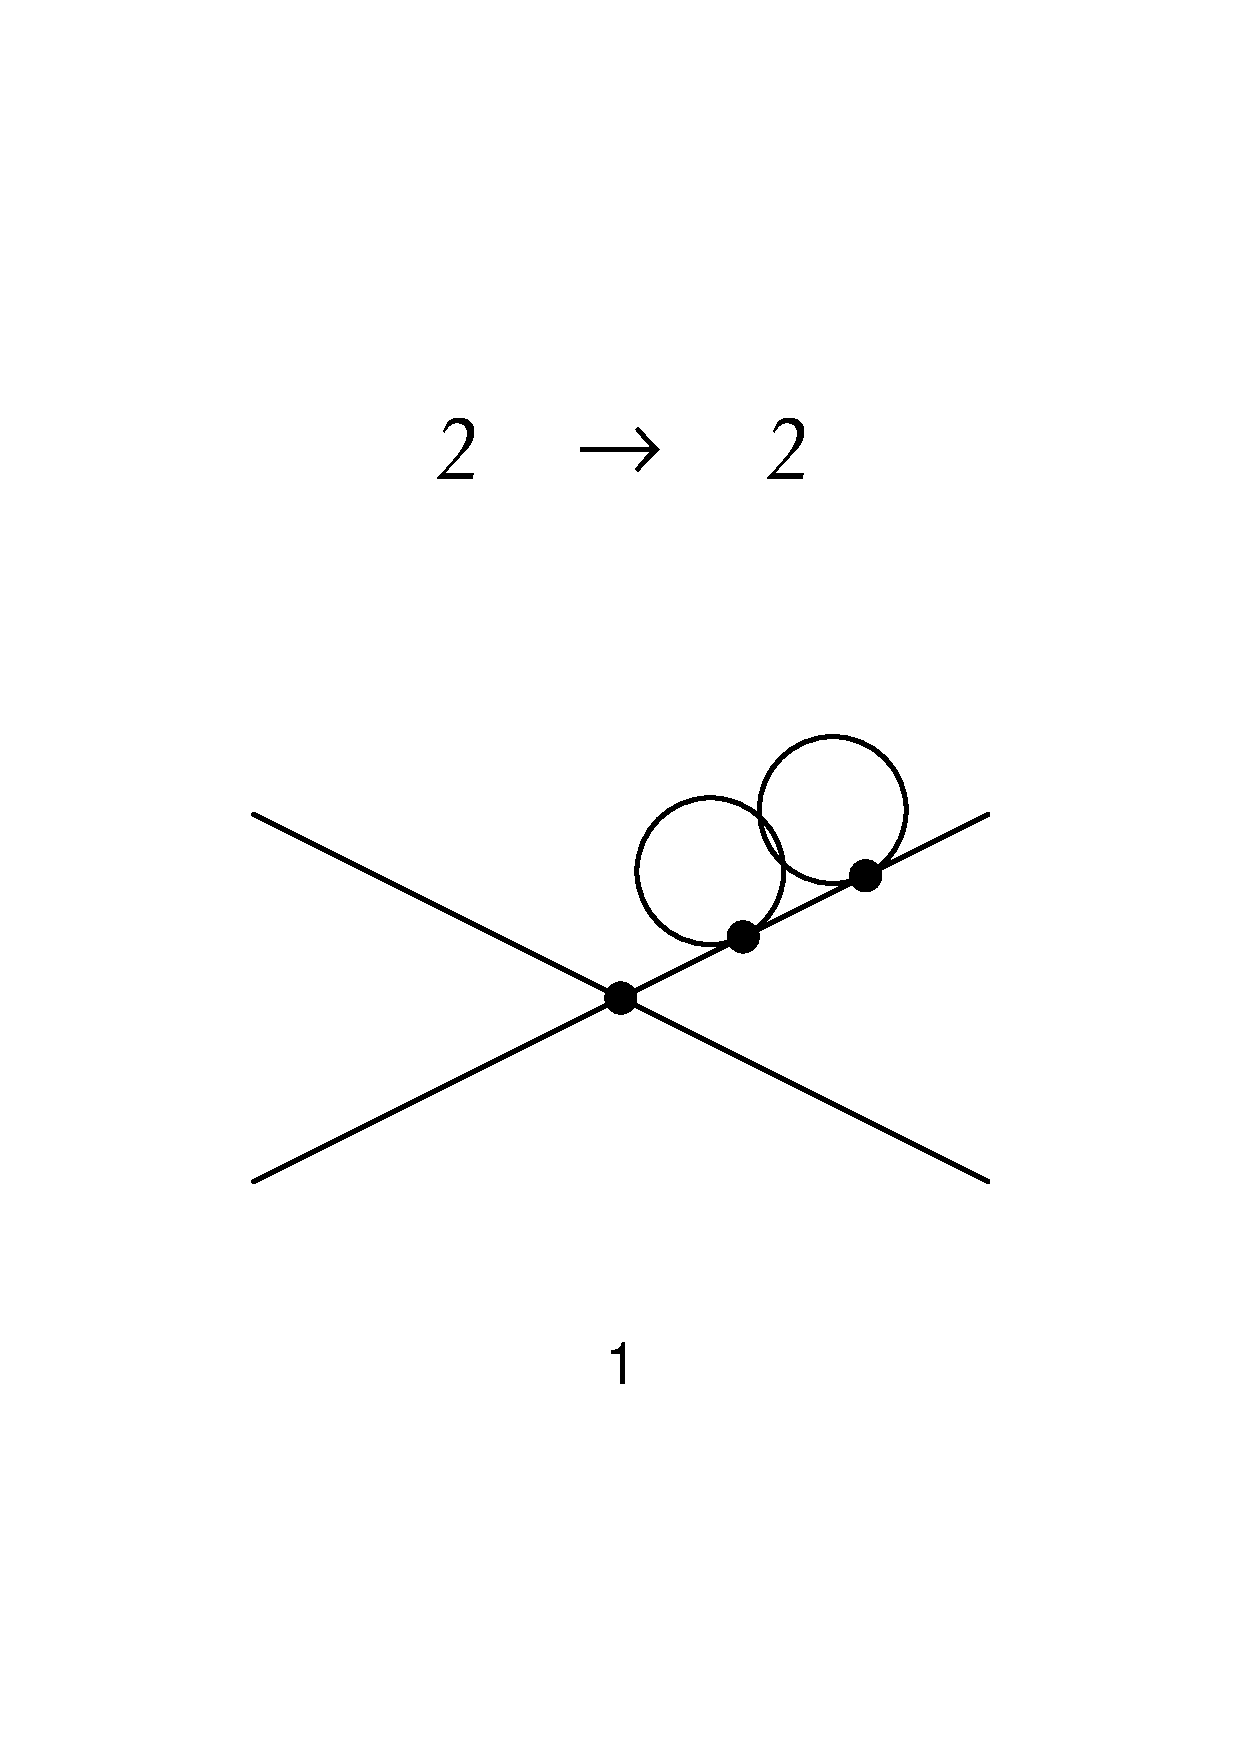
\includegraphics[width=0.28\textwidth]{generated/L2/images/topology30.pdf}
\end{center}
\noindent Parsed propagators: 8. Internal vertices: 3. Internal half-edges: 12.\\
\noindent Assignments checked: 32768. Surviving (nonzero vertex weight): 4096.\\
\noindent Raw $N_c$ power: 2. Net power in $C(t)$: -2.
\[\text{No surviving SK contributions for this topology.}\]
\section*{Topology 31 (FeynArts Topology 4)}
\begin{center}
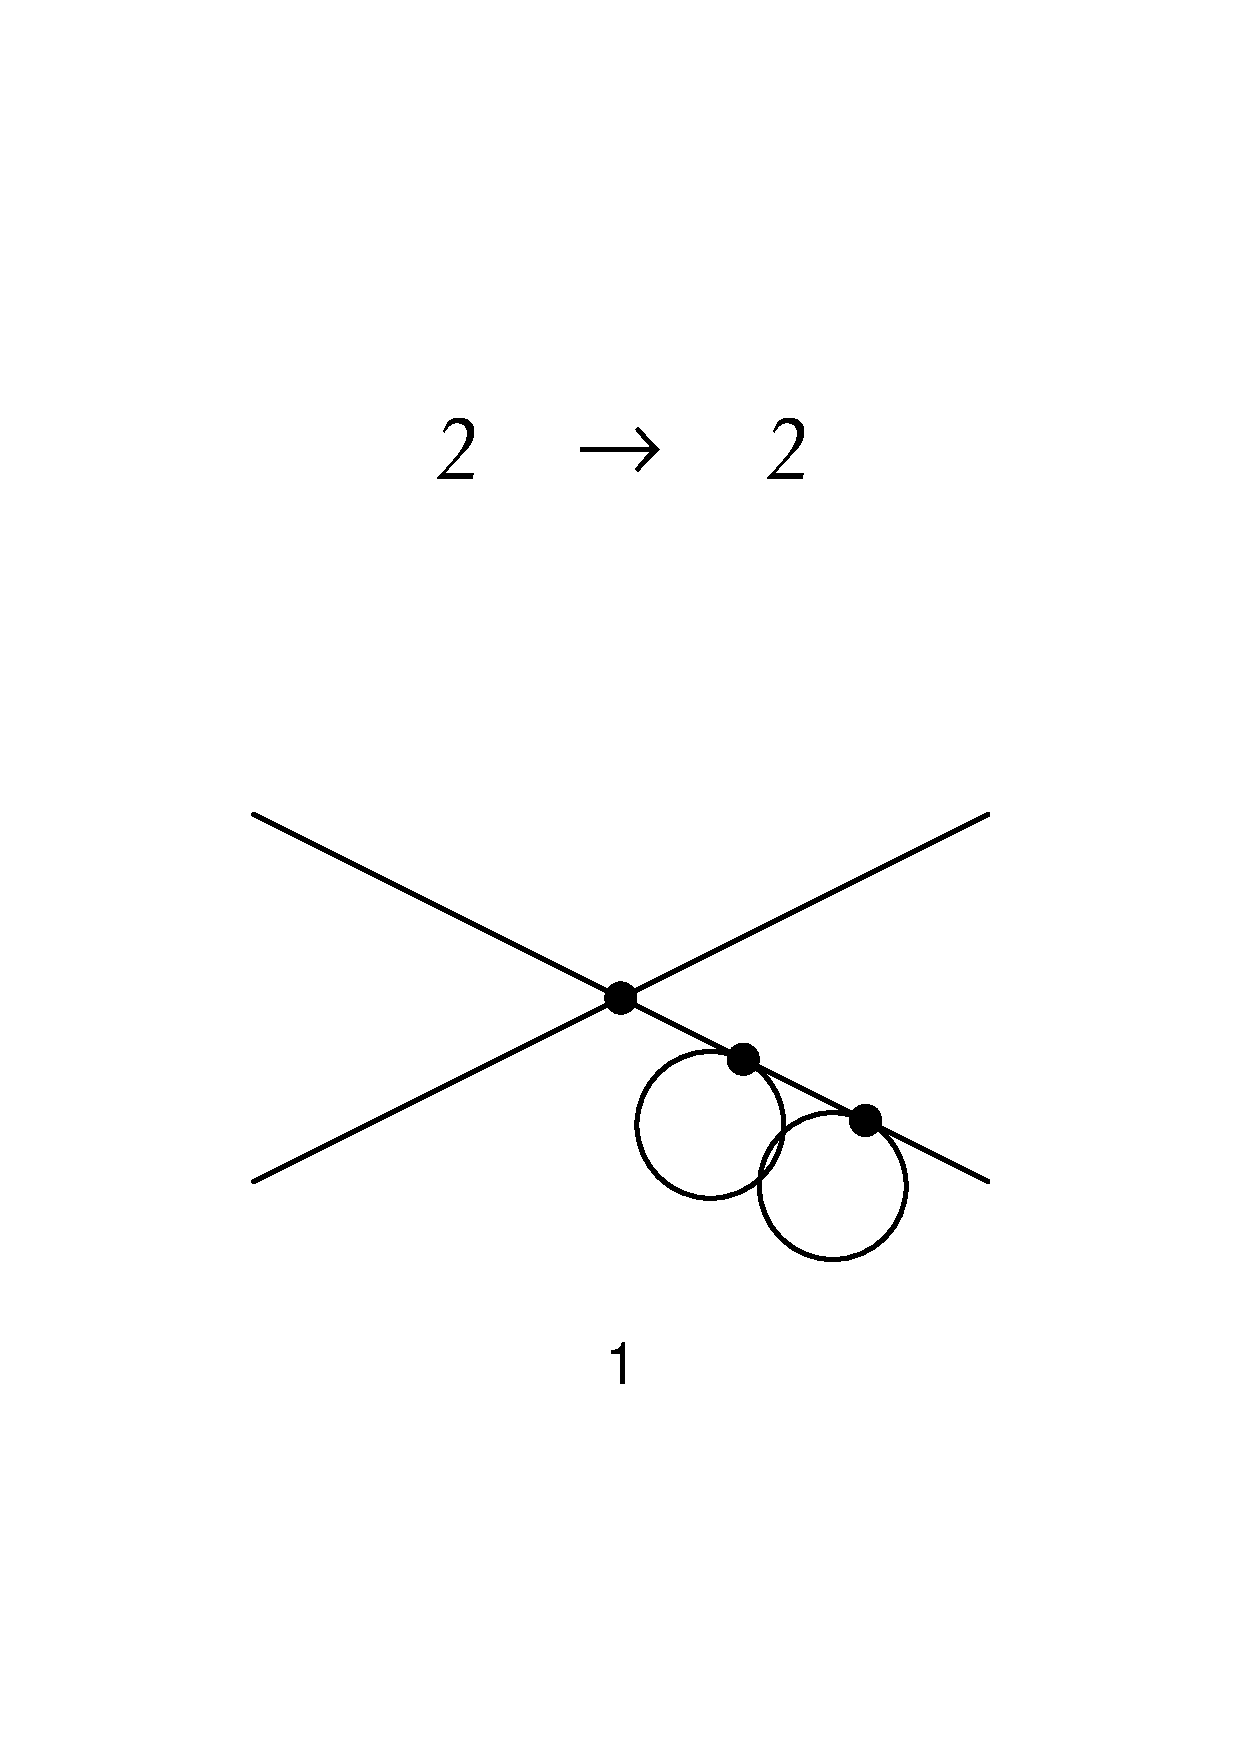
\includegraphics[width=0.28\textwidth]{generated/L2/images/topology31.pdf}
\end{center}
\noindent Parsed propagators: 8. Internal vertices: 3. Internal half-edges: 12.\\
\noindent Assignments checked: 32768. Surviving (nonzero vertex weight): 4096.\\
\noindent Raw $N_c$ power: 2. Net power in $C(t)$: -2.
\noindent Explicit surviving terms:
\begin{equation*}
\mathcal{T}_{31,1} = 64 i g_{2}^{3}\,N_c^{-2}\,G^<\left(z_{3},z_{2}\right) \, G^>\left(x_3,z_{1}\right) \, G_A\left(x_2,z_{1}\right) \, G_A\left(x_4,z_{2}\right) \, G_A\left(z_{2},z_{2}\right) \, G_A\left(z_{3},z_{1}\right) \, G_K\left(z_{3},z_{3}\right) \, G_R\left(x_1,z_{1}\right)
\end{equation*}
\begin{equation*}
\mathcal{T}_{31,2} = 64 i g_{2}^{3}\,N_c^{-2}\,G^<\left(z_{3},z_{2}\right) \, G^>\left(x_3,z_{1}\right) \, G_A\left(x_2,z_{1}\right) \, G_A\left(x_4,z_{2}\right) \, G_A\left(z_{2},z_{2}\right) \, G_A\left(z_{3},z_{3}\right) \, G_K\left(x_1,z_{1}\right) \, G_R\left(z_{3},z_{1}\right)
\end{equation*}
\begin{equation*}
\mathcal{T}_{31,3} = 64 i g_{2}^{3}\,N_c^{-2}\,G^<\left(z_{3},z_{2}\right) \, G^>\left(x_3,z_{1}\right) \, G_A\left(x_2,z_{1}\right) \, G_A\left(x_4,z_{2}\right) \, G_A\left(z_{2},z_{2}\right) \, G_A\left(z_{3},z_{3}\right) \, G_K\left(z_{3},z_{1}\right) \, G_R\left(x_1,z_{1}\right)
\end{equation*}
\begin{equation*}
\mathcal{T}_{31,4} = 64 i g_{2}^{3}\,N_c^{-2}\,G^<\left(z_{3},z_{2}\right) \, G^>\left(x_3,z_{1}\right) \, G_A\left(x_2,z_{1}\right) \, G_A\left(x_4,z_{2}\right) \, G_A\left(z_{2},z_{2}\right) \, G_K\left(x_1,z_{1}\right) \, G_R\left(z_{3},z_{1}\right) \, G_R\left(z_{3},z_{3}\right)
\end{equation*}
\begin{equation*}
\mathcal{T}_{31,5} = 64 i g_{2}^{3}\,N_c^{-2}\,G^<\left(z_{3},z_{2}\right) \, G^>\left(x_3,z_{1}\right) \, G_A\left(x_2,z_{1}\right) \, G_A\left(x_4,z_{2}\right) \, G_A\left(z_{2},z_{2}\right) \, G_K\left(z_{3},z_{1}\right) \, G_R\left(x_1,z_{1}\right) \, G_R\left(z_{3},z_{3}\right)
\end{equation*}
\begin{equation*}
\mathcal{T}_{31,6} = 64 i g_{2}^{3}\,N_c^{-2}\,G^<\left(z_{3},z_{2}\right) \, G^>\left(x_3,z_{1}\right) \, G_A\left(x_2,z_{1}\right) \, G_A\left(x_4,z_{2}\right) \, G_A\left(z_{3},z_{1}\right) \, G_K\left(z_{3},z_{3}\right) \, G_R\left(x_1,z_{1}\right) \, G_R\left(z_{2},z_{2}\right)
\end{equation*}
\begin{equation*}
\mathcal{T}_{31,7} = 64 i g_{2}^{3}\,N_c^{-2}\,G^<\left(z_{3},z_{2}\right) \, G^>\left(x_3,z_{1}\right) \, G_A\left(x_2,z_{1}\right) \, G_A\left(x_4,z_{2}\right) \, G_A\left(z_{3},z_{3}\right) \, G_K\left(x_1,z_{1}\right) \, G_R\left(z_{2},z_{2}\right) \, G_R\left(z_{3},z_{1}\right)
\end{equation*}
\begin{equation*}
\mathcal{T}_{31,8} = 64 i g_{2}^{3}\,N_c^{-2}\,G^<\left(z_{3},z_{2}\right) \, G^>\left(x_3,z_{1}\right) \, G_A\left(x_2,z_{1}\right) \, G_A\left(x_4,z_{2}\right) \, G_A\left(z_{3},z_{3}\right) \, G_K\left(z_{3},z_{1}\right) \, G_R\left(x_1,z_{1}\right) \, G_R\left(z_{2},z_{2}\right)
\end{equation*}
\begin{equation*}
\mathcal{T}_{31,9} = 64 i g_{2}^{3}\,N_c^{-2}\,G^<\left(z_{3},z_{2}\right) \, G^>\left(x_3,z_{1}\right) \, G_A\left(x_2,z_{1}\right) \, G_A\left(x_4,z_{2}\right) \, G_K\left(x_1,z_{1}\right) \, G_R\left(z_{2},z_{2}\right) \, G_R\left(z_{3},z_{1}\right) \, G_R\left(z_{3},z_{3}\right)
\end{equation*}
\begin{equation*}
\mathcal{T}_{31,10} = 64 i g_{2}^{3}\,N_c^{-2}\,G^<\left(z_{3},z_{2}\right) \, G^>\left(x_3,z_{1}\right) \, G_A\left(x_2,z_{1}\right) \, G_A\left(x_4,z_{2}\right) \, G_K\left(z_{3},z_{1}\right) \, G_R\left(x_1,z_{1}\right) \, G_R\left(z_{2},z_{2}\right) \, G_R\left(z_{3},z_{3}\right)
\end{equation*}
\begin{equation*}
\mathcal{T}_{31,11} = 64 i g_{2}^{3}\,N_c^{-2}\,G^>\left(x_3,z_{1}\right) \, G^>\left(z_{3},z_{1}\right) \, G_A\left(x_2,z_{1}\right) \, G_A\left(x_4,z_{2}\right) \, G_A\left(z_{2},z_{2}\right) \, G_A\left(z_{3},z_{2}\right) \, G_K\left(z_{3},z_{3}\right) \, G_R\left(x_1,z_{1}\right)
\end{equation*}
\begin{equation*}
\mathcal{T}_{31,12} = 64 i g_{2}^{3}\,N_c^{-2}\,G^>\left(x_3,z_{1}\right) \, G^>\left(z_{3},z_{1}\right) \, G_A\left(x_2,z_{1}\right) \, G_A\left(x_4,z_{2}\right) \, G_A\left(z_{2},z_{2}\right) \, G_A\left(z_{3},z_{3}\right) \, G_K\left(z_{3},z_{2}\right) \, G_R\left(x_1,z_{1}\right)
\end{equation*}
\begin{equation*}
\mathcal{T}_{31,13} = 64 i g_{2}^{3}\,N_c^{-2}\,G^>\left(x_3,z_{1}\right) \, G^>\left(z_{3},z_{1}\right) \, G_A\left(x_2,z_{1}\right) \, G_A\left(x_4,z_{2}\right) \, G_A\left(z_{2},z_{2}\right) \, G_K\left(z_{3},z_{2}\right) \, G_R\left(x_1,z_{1}\right) \, G_R\left(z_{3},z_{3}\right)
\end{equation*}
\begin{equation*}
\mathcal{T}_{31,14} = 64 i g_{2}^{3}\,N_c^{-2}\,G^>\left(x_3,z_{1}\right) \, G^>\left(z_{3},z_{1}\right) \, G_A\left(x_2,z_{1}\right) \, G_A\left(x_4,z_{2}\right) \, G_A\left(z_{3},z_{2}\right) \, G_K\left(z_{3},z_{3}\right) \, G_R\left(x_1,z_{1}\right) \, G_R\left(z_{2},z_{2}\right)
\end{equation*}
\begin{equation*}
\mathcal{T}_{31,15} = 64 i g_{2}^{3}\,N_c^{-2}\,G^>\left(x_3,z_{1}\right) \, G^>\left(z_{3},z_{1}\right) \, G_A\left(x_2,z_{1}\right) \, G_A\left(x_4,z_{2}\right) \, G_A\left(z_{3},z_{3}\right) \, G_K\left(z_{2},z_{2}\right) \, G_R\left(x_1,z_{1}\right) \, G_R\left(z_{3},z_{2}\right)
\end{equation*}
\begin{equation*}
\mathcal{T}_{31,16} = 64 i g_{2}^{3}\,N_c^{-2}\,G^>\left(x_3,z_{1}\right) \, G^>\left(z_{3},z_{1}\right) \, G_A\left(x_2,z_{1}\right) \, G_A\left(x_4,z_{2}\right) \, G_A\left(z_{3},z_{3}\right) \, G_K\left(z_{3},z_{2}\right) \, G_R\left(x_1,z_{1}\right) \, G_R\left(z_{2},z_{2}\right)
\end{equation*}
\begin{equation*}
\mathcal{T}_{31,17} = 64 i g_{2}^{3}\,N_c^{-2}\,G^>\left(x_3,z_{1}\right) \, G^>\left(z_{3},z_{1}\right) \, G_A\left(x_2,z_{1}\right) \, G_A\left(x_4,z_{2}\right) \, G_K\left(z_{2},z_{2}\right) \, G_R\left(x_1,z_{1}\right) \, G_R\left(z_{3},z_{2}\right) \, G_R\left(z_{3},z_{3}\right)
\end{equation*}
\begin{equation*}
\mathcal{T}_{31,18} = 64 i g_{2}^{3}\,N_c^{-2}\,G^>\left(x_3,z_{1}\right) \, G^>\left(z_{3},z_{1}\right) \, G_A\left(x_2,z_{1}\right) \, G_A\left(x_4,z_{2}\right) \, G_K\left(z_{3},z_{2}\right) \, G_R\left(x_1,z_{1}\right) \, G_R\left(z_{2},z_{2}\right) \, G_R\left(z_{3},z_{3}\right)
\end{equation*}
\section*{Topology 32 (FeynArts Topology 4)}
\begin{center}
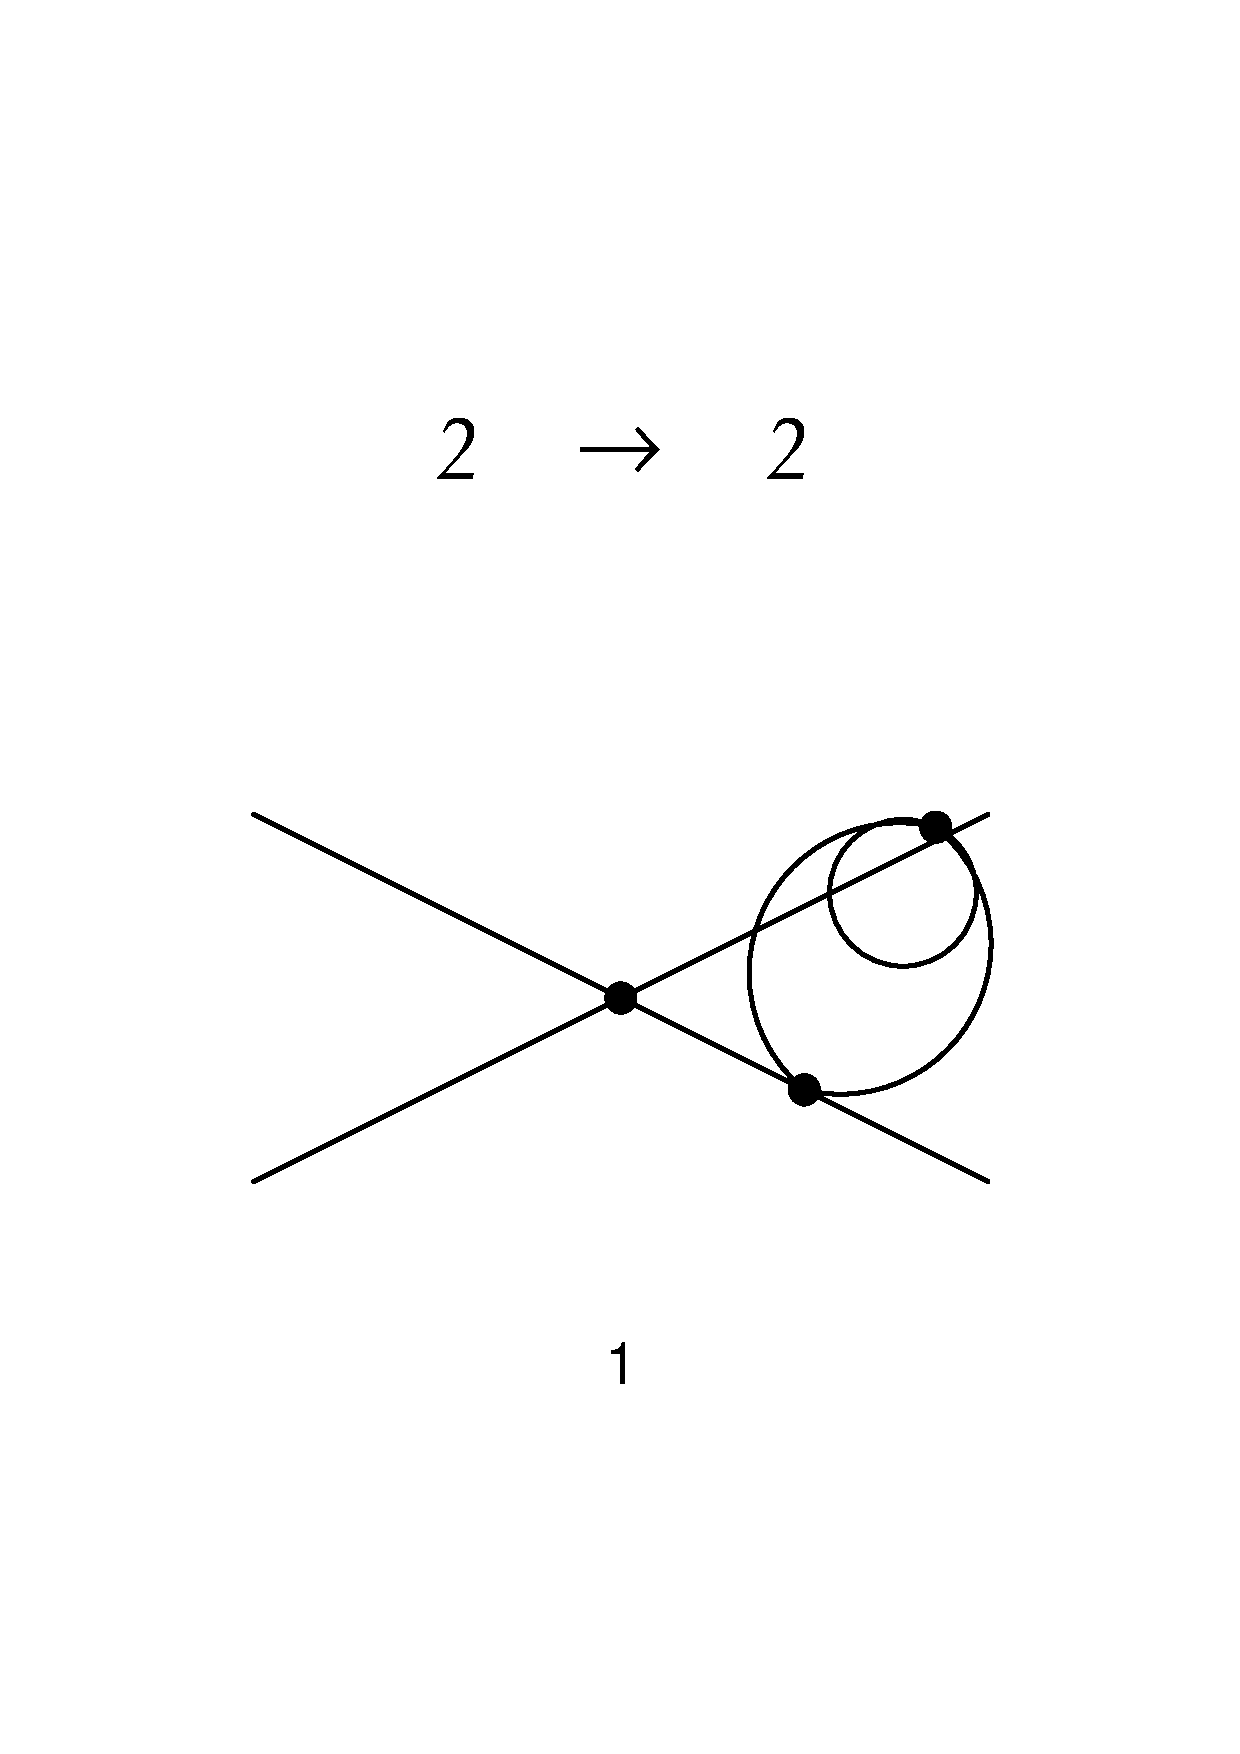
\includegraphics[width=0.28\textwidth]{generated/L2/images/topology32.pdf}
\end{center}
\noindent Parsed propagators: 8. Internal vertices: 3. Internal half-edges: 12.\\
\noindent Assignments checked: 32768. Surviving (nonzero vertex weight): 4096.\\
\noindent Raw $N_c$ power: 2. Net power in $C(t)$: -2.
\noindent Explicit surviving terms:
\begin{equation*}
\mathcal{T}_{32,1} = 128 i g_{2}^{3}\,N_c^{-2}\,G^<\left(z_{1},z_{2}\right) \, G^>\left(x_3,z_{1}\right) \, G_A\left(x_2,z_{1}\right) \, G_A\left(x_4,z_{2}\right) \, G_A\left(z_{2},z_{3}\right) \, G_A\left(z_{3},z_{3}\right) \, G_K\left(z_{2},z_{3}\right) \, G_R\left(x_1,z_{1}\right)
\end{equation*}
\begin{equation*}
\mathcal{T}_{32,2} = 128 i g_{2}^{3}\,N_c^{-2}\,G^<\left(z_{1},z_{2}\right) \, G^>\left(x_3,z_{1}\right) \, G_A\left(x_2,z_{1}\right) \, G_A\left(x_4,z_{2}\right) \, G_A\left(z_{2},z_{3}\right) \, G_K\left(z_{2},z_{3}\right) \, G_R\left(x_1,z_{1}\right) \, G_R\left(z_{3},z_{3}\right)
\end{equation*}
\begin{equation*}
\mathcal{T}_{32,3} = 128 i g_{2}^{3}\,N_c^{-2}\,G^<\left(z_{1},z_{2}\right) \, G^>\left(x_3,z_{1}\right) \, G_A\left(x_2,z_{1}\right) \, G_A\left(x_4,z_{2}\right) \, G_A\left(z_{2},z_{3}\right) \, G_K\left(z_{3},z_{3}\right) \, G_R\left(x_1,z_{1}\right) \, G_R\left(z_{2},z_{3}\right)
\end{equation*}
\section*{Topology 33 (FeynArts Topology 4)}
\begin{center}
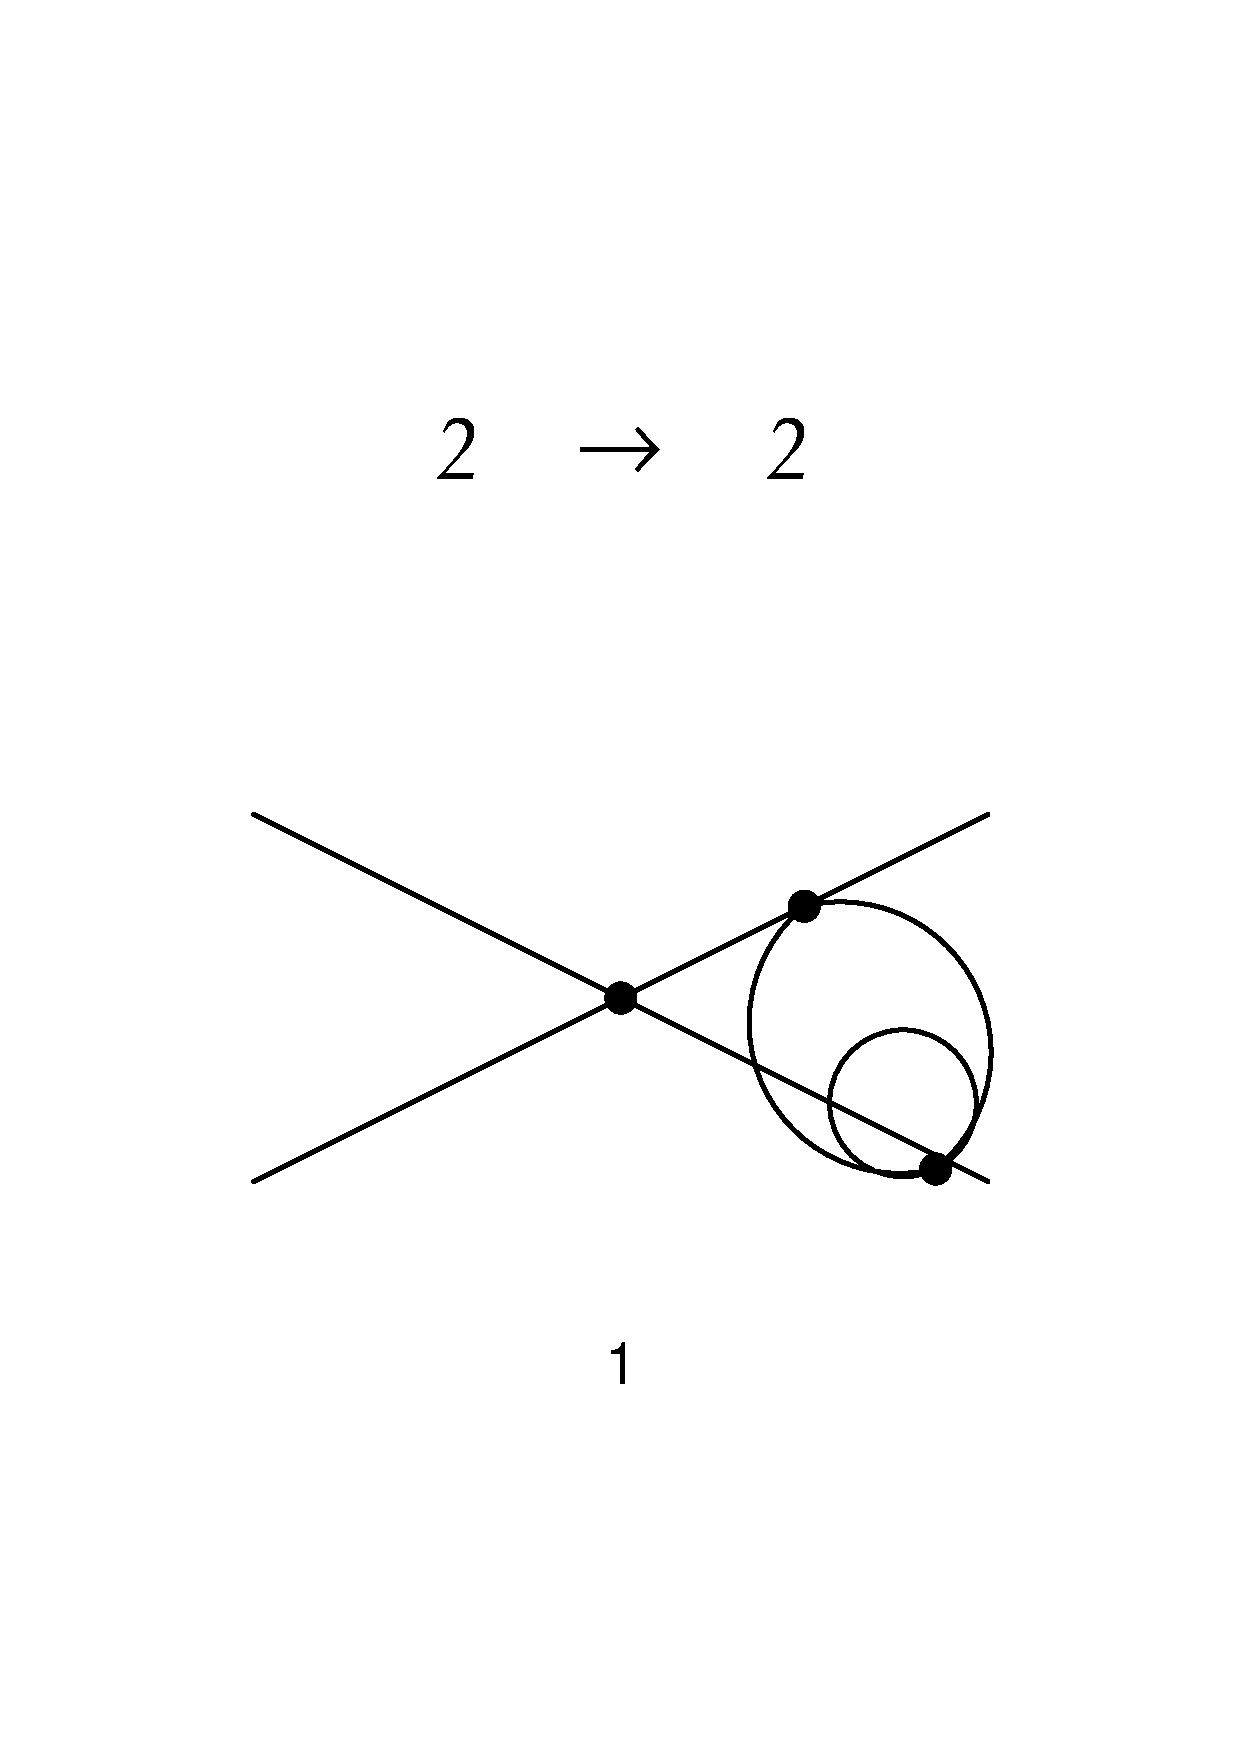
\includegraphics[width=0.28\textwidth]{generated/L2/images/topology33.pdf}
\end{center}
\noindent Parsed propagators: 8. Internal vertices: 3. Internal half-edges: 12.\\
\noindent Assignments checked: 32768. Surviving (nonzero vertex weight): 4096.\\
\noindent Raw $N_c$ power: 2. Net power in $C(t)$: -2.
\[\text{No surviving SK contributions for this topology.}\]
\section*{Topology 34 (FeynArts Topology 4)}
\begin{center}
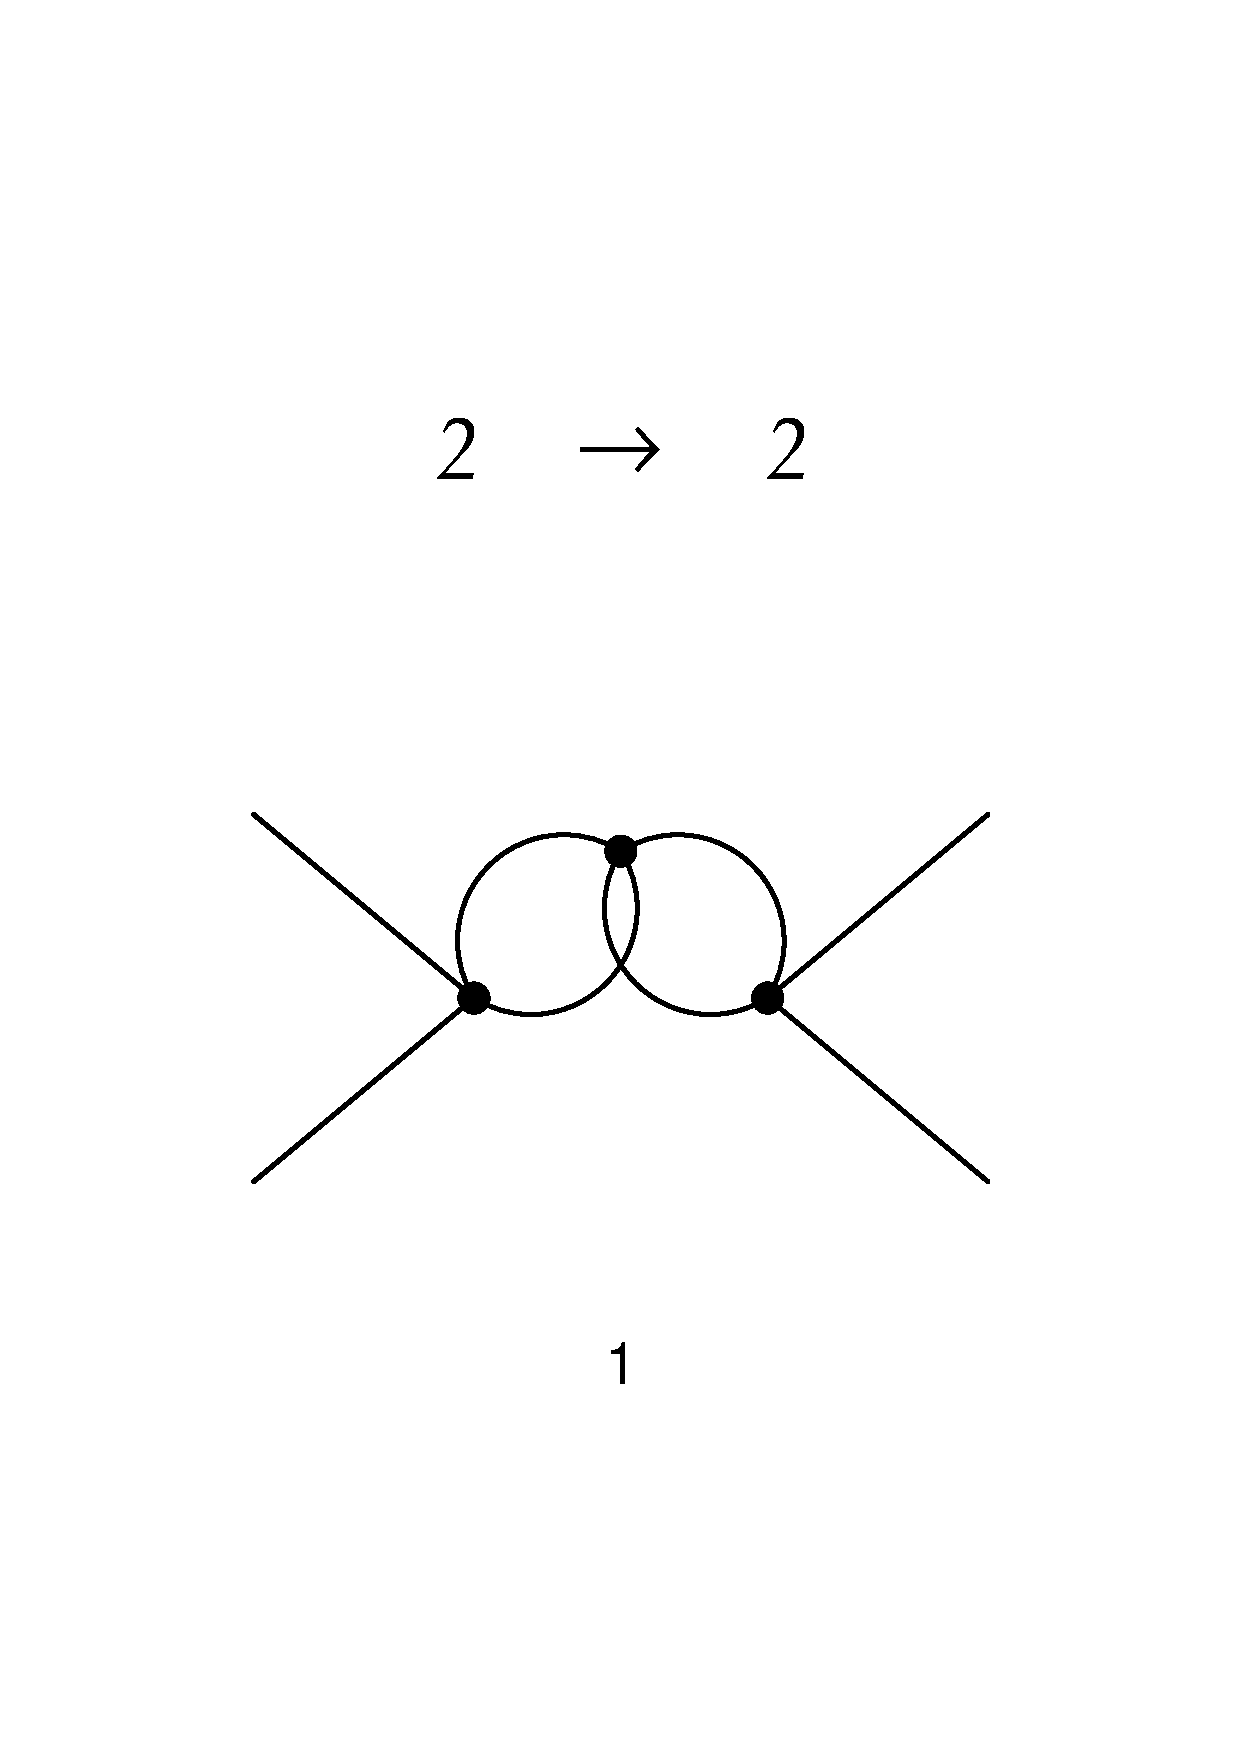
\includegraphics[width=0.28\textwidth]{generated/L2/images/topology34.pdf}
\end{center}
\noindent Parsed propagators: 8. Internal vertices: 3. Internal half-edges: 12.\\
\noindent Assignments checked: 32768. Surviving (nonzero vertex weight): 4096.\\
\noindent Raw $N_c$ power: 1. Net power in $C(t)$: -3.
\noindent Explicit surviving terms:
\begin{equation*}
\mathcal{T}_{34,1} = 128 i g_{2}^{3}\,N_c^{-3}\,G^<\left(z_{1},z_{3}\right) \, G^<\left(z_{1},z_{3}\right) \, G_A\left(x_2,z_{1}\right) \, G_A\left(x_4,z_{2}\right) \, G_A\left(z_{2},z_{3}\right) \, G_K\left(x_3,z_{2}\right) \, G_R\left(x_1,z_{1}\right) \, G_R\left(z_{2},z_{3}\right)
\end{equation*}
\begin{equation*}
\mathcal{T}_{34,2} = 128 i g_{2}^{3}\,N_c^{-3}\,G^<\left(z_{1},z_{3}\right) \, G^<\left(z_{1},z_{3}\right) \, G_A\left(x_2,z_{1}\right) \, G_A\left(x_4,z_{2}\right) \, G_K\left(z_{2},z_{3}\right) \, G_R\left(x_1,z_{1}\right) \, G_R\left(x_3,z_{2}\right) \, G_R\left(z_{2},z_{3}\right)
\end{equation*}
\begin{equation*}
\mathcal{T}_{34,3} = 128 i g_{2}^{3}\,N_c^{-3}\,G^>\left(z_{2},z_{3}\right) \, G^>\left(z_{2},z_{3}\right) \, G_A\left(x_2,z_{1}\right) \, G_A\left(x_4,z_{2}\right) \, G_A\left(z_{1},z_{3}\right) \, G_K\left(x_1,z_{1}\right) \, G_R\left(x_3,z_{2}\right) \, G_R\left(z_{1},z_{3}\right)
\end{equation*}
\begin{equation*}
\mathcal{T}_{34,4} = 128 i g_{2}^{3}\,N_c^{-3}\,G^>\left(z_{2},z_{3}\right) \, G^>\left(z_{2},z_{3}\right) \, G_A\left(x_2,z_{1}\right) \, G_A\left(x_4,z_{2}\right) \, G_K\left(z_{1},z_{3}\right) \, G_R\left(x_1,z_{1}\right) \, G_R\left(x_3,z_{2}\right) \, G_R\left(z_{1},z_{3}\right)
\end{equation*}
\section*{Topology 35 (FeynArts Topology 4)}
\begin{center}
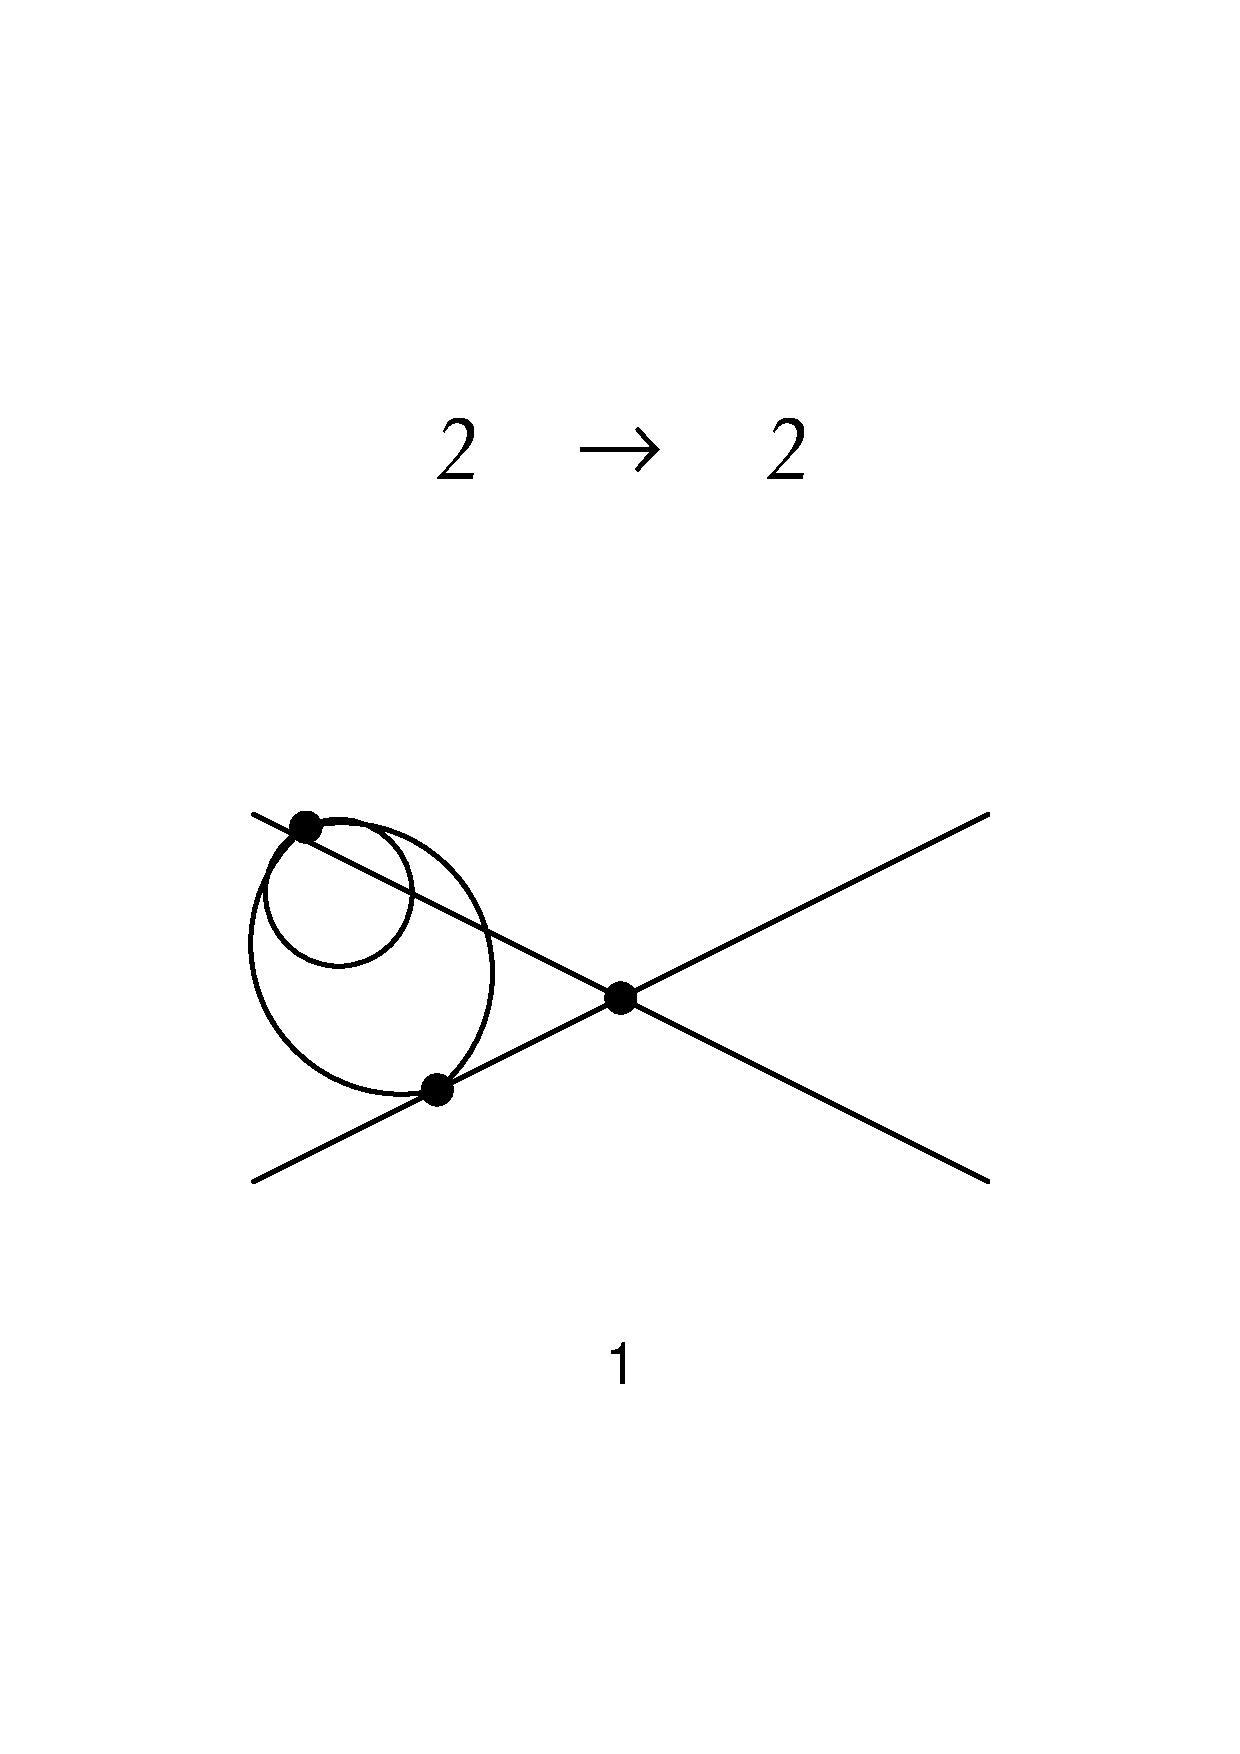
\includegraphics[width=0.28\textwidth]{generated/L2/images/topology35.pdf}
\end{center}
\noindent Parsed propagators: 8. Internal vertices: 3. Internal half-edges: 12.\\
\noindent Assignments checked: 32768. Surviving (nonzero vertex weight): 4096.\\
\noindent Raw $N_c$ power: 2. Net power in $C(t)$: -2.
\noindent Explicit surviving terms:
\begin{equation*}
\mathcal{T}_{35,1} = 128 i g_{2}^{3}\,N_c^{-2}\,G^<\left(x_1,z_{1}\right) \, G^>\left(z_{1},z_{2}\right) \, G_A\left(x_2,z_{2}\right) \, G_A\left(x_4,z_{1}\right) \, G_A\left(z_{2},z_{3}\right) \, G_A\left(z_{3},z_{3}\right) \, G_K\left(z_{2},z_{3}\right) \, G_R\left(x_3,z_{1}\right)
\end{equation*}
\begin{equation*}
\mathcal{T}_{35,2} = 128 i g_{2}^{3}\,N_c^{-2}\,G^<\left(x_1,z_{1}\right) \, G^>\left(z_{1},z_{2}\right) \, G_A\left(x_2,z_{2}\right) \, G_A\left(x_4,z_{1}\right) \, G_A\left(z_{2},z_{3}\right) \, G_K\left(z_{2},z_{3}\right) \, G_R\left(x_3,z_{1}\right) \, G_R\left(z_{3},z_{3}\right)
\end{equation*}
\begin{equation*}
\mathcal{T}_{35,3} = 128 i g_{2}^{3}\,N_c^{-2}\,G^<\left(x_1,z_{1}\right) \, G^>\left(z_{1},z_{2}\right) \, G_A\left(x_2,z_{2}\right) \, G_A\left(x_4,z_{1}\right) \, G_A\left(z_{2},z_{3}\right) \, G_K\left(z_{3},z_{3}\right) \, G_R\left(x_3,z_{1}\right) \, G_R\left(z_{2},z_{3}\right)
\end{equation*}
\section*{Topology 36 (FeynArts Topology 4)}
\begin{center}
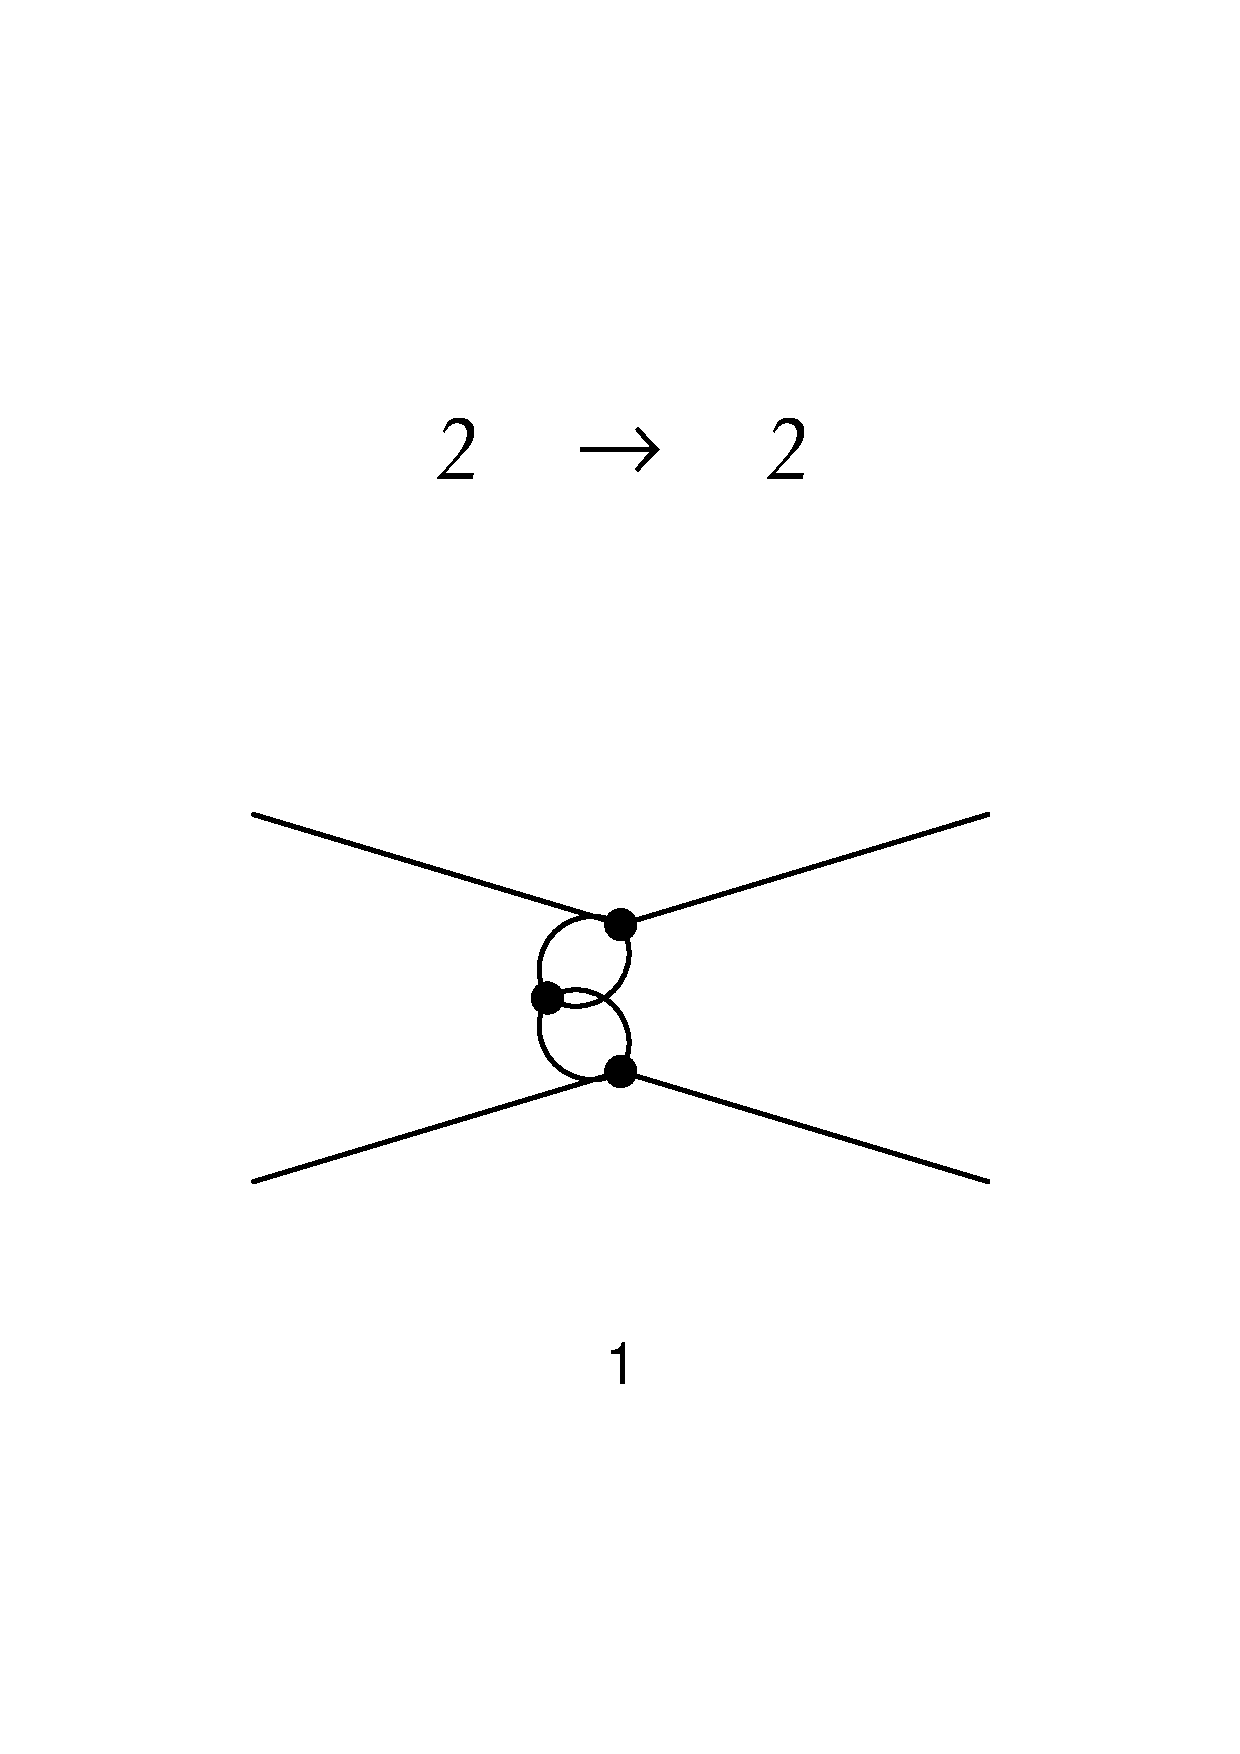
\includegraphics[width=0.28\textwidth]{generated/L2/images/topology36.pdf}
\end{center}
\noindent Parsed propagators: 8. Internal vertices: 3. Internal half-edges: 12.\\
\noindent Assignments checked: 32768. Surviving (nonzero vertex weight): 4096.\\
\noindent Raw $N_c$ power: 1. Net power in $C(t)$: -3.
\[\text{No surviving SK contributions for this topology.}\]
\section*{Topology 37 (FeynArts Topology 4)}
\begin{center}
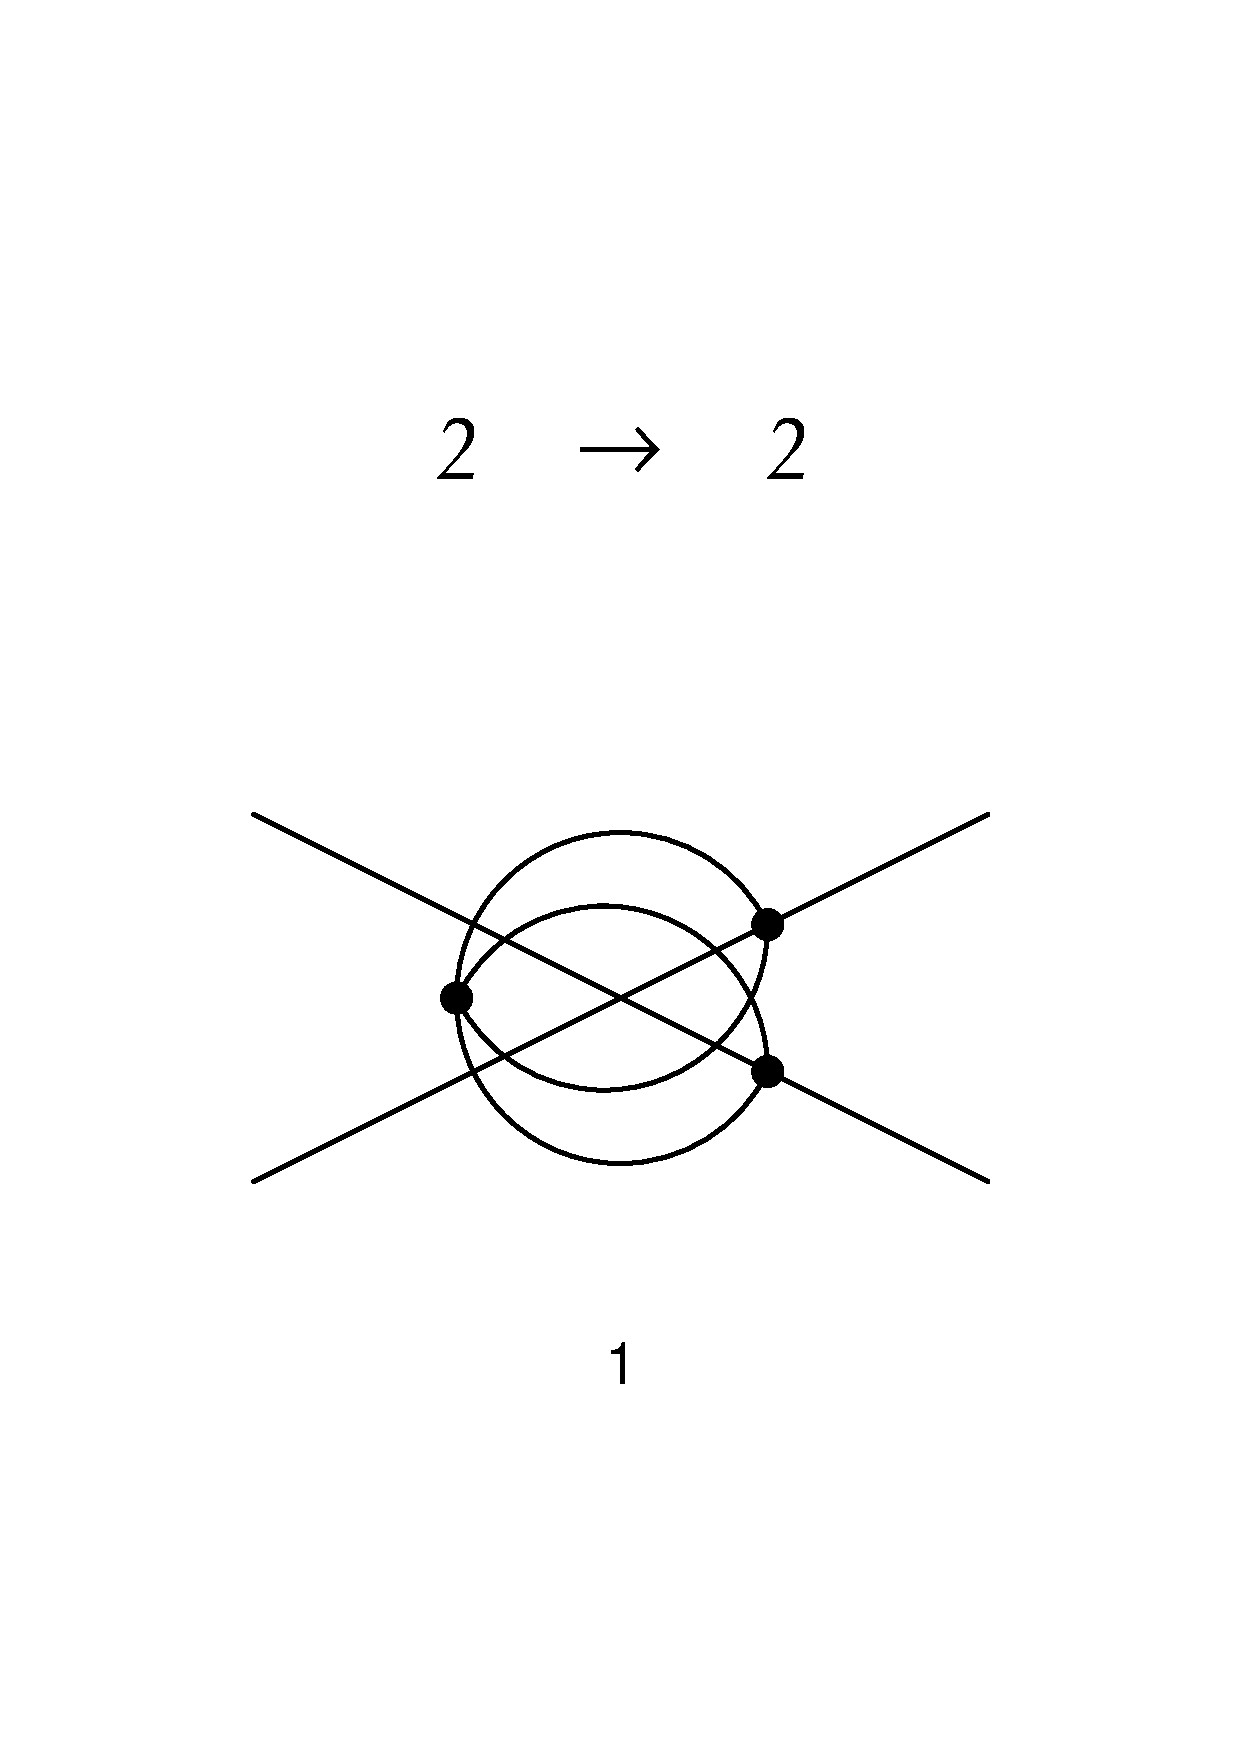
\includegraphics[width=0.28\textwidth]{generated/L2/images/topology37.pdf}
\end{center}
\noindent Parsed propagators: 8. Internal vertices: 3. Internal half-edges: 12.\\
\noindent Assignments checked: 32768. Surviving (nonzero vertex weight): 4096.\\
\noindent Raw $N_c$ power: 1. Net power in $C(t)$: -3.
\[\text{No surviving SK contributions for this topology.}\]
\section*{Topology 38 (FeynArts Topology 4)}
\begin{center}
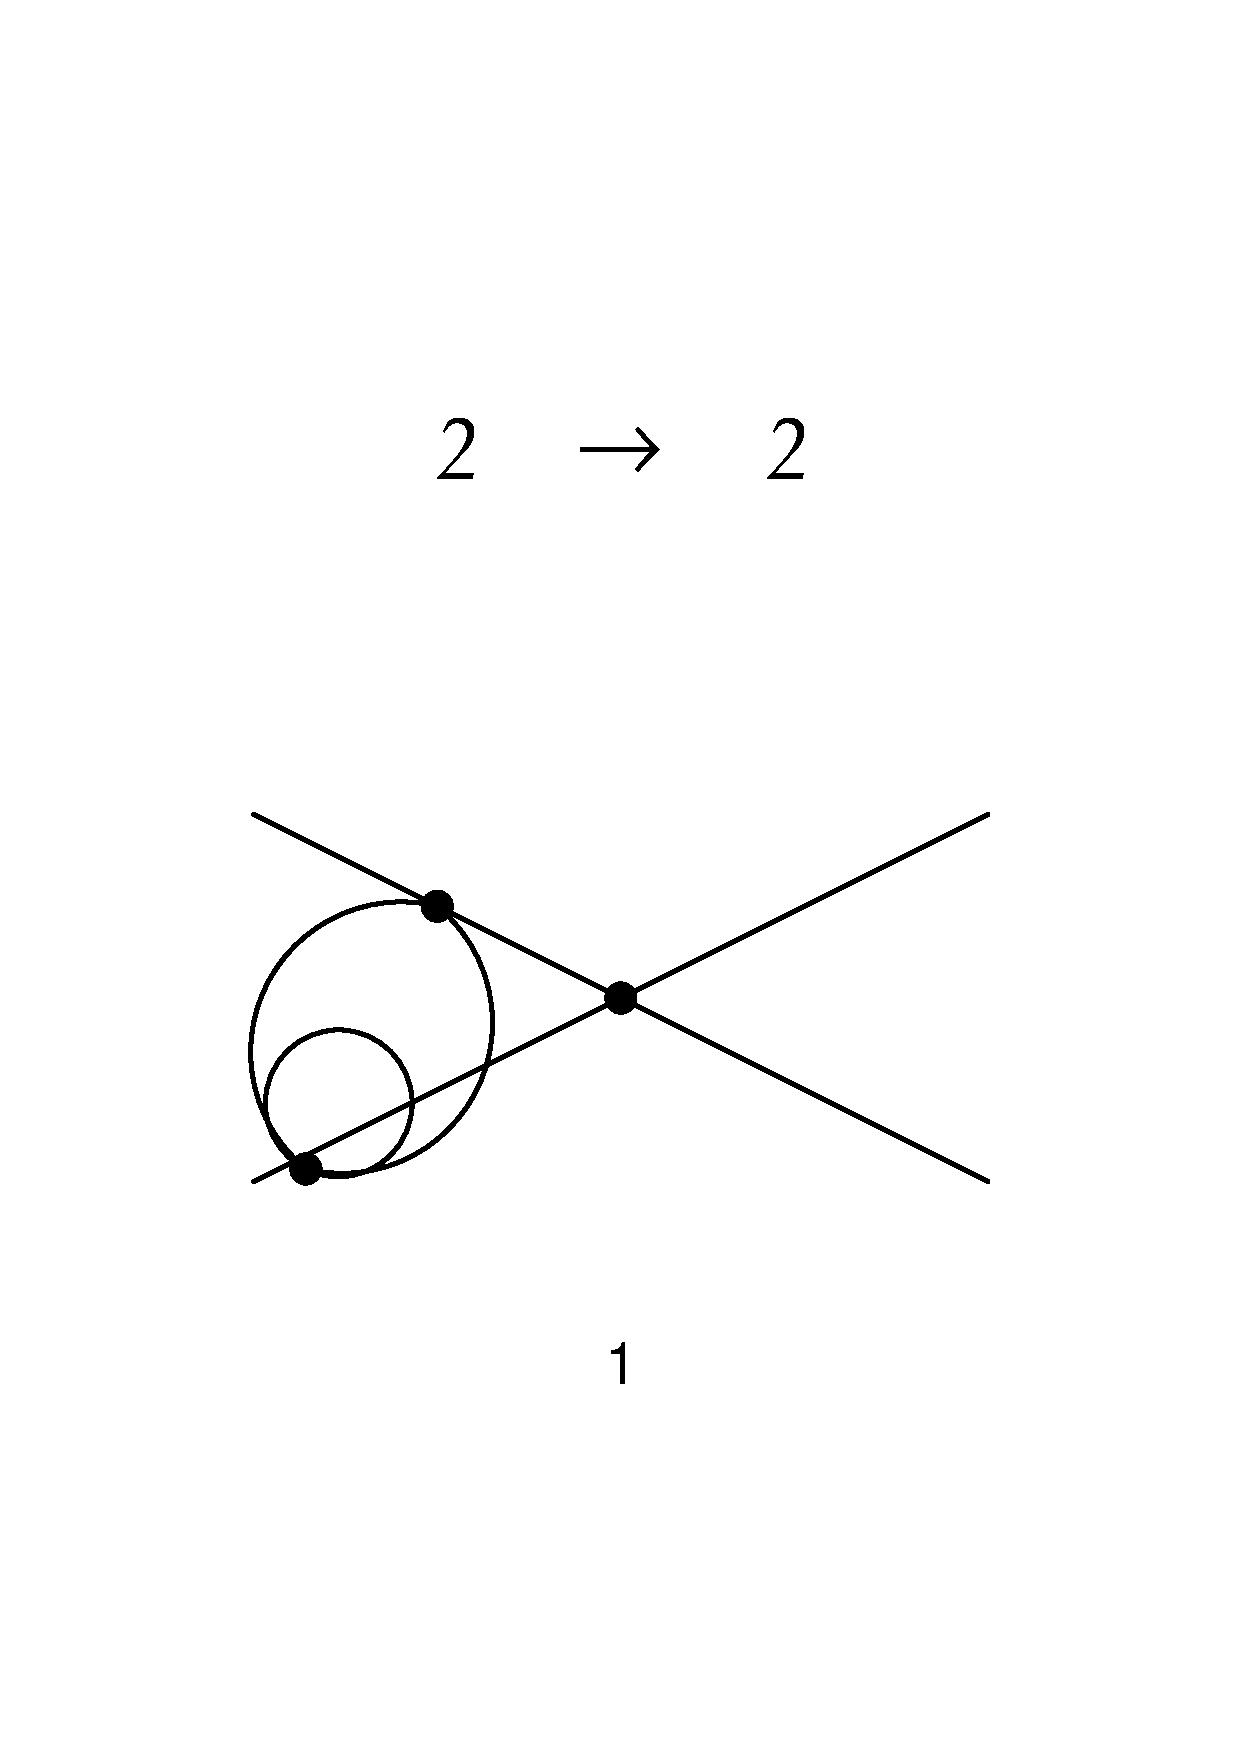
\includegraphics[width=0.28\textwidth]{generated/L2/images/topology38.pdf}
\end{center}
\noindent Parsed propagators: 8. Internal vertices: 3. Internal half-edges: 12.\\
\noindent Assignments checked: 32768. Surviving (nonzero vertex weight): 4096.\\
\noindent Raw $N_c$ power: 2. Net power in $C(t)$: -2.
\[\text{No surviving SK contributions for this topology.}\]
\section*{Topology 39 (FeynArts Topology 6)}
\begin{center}
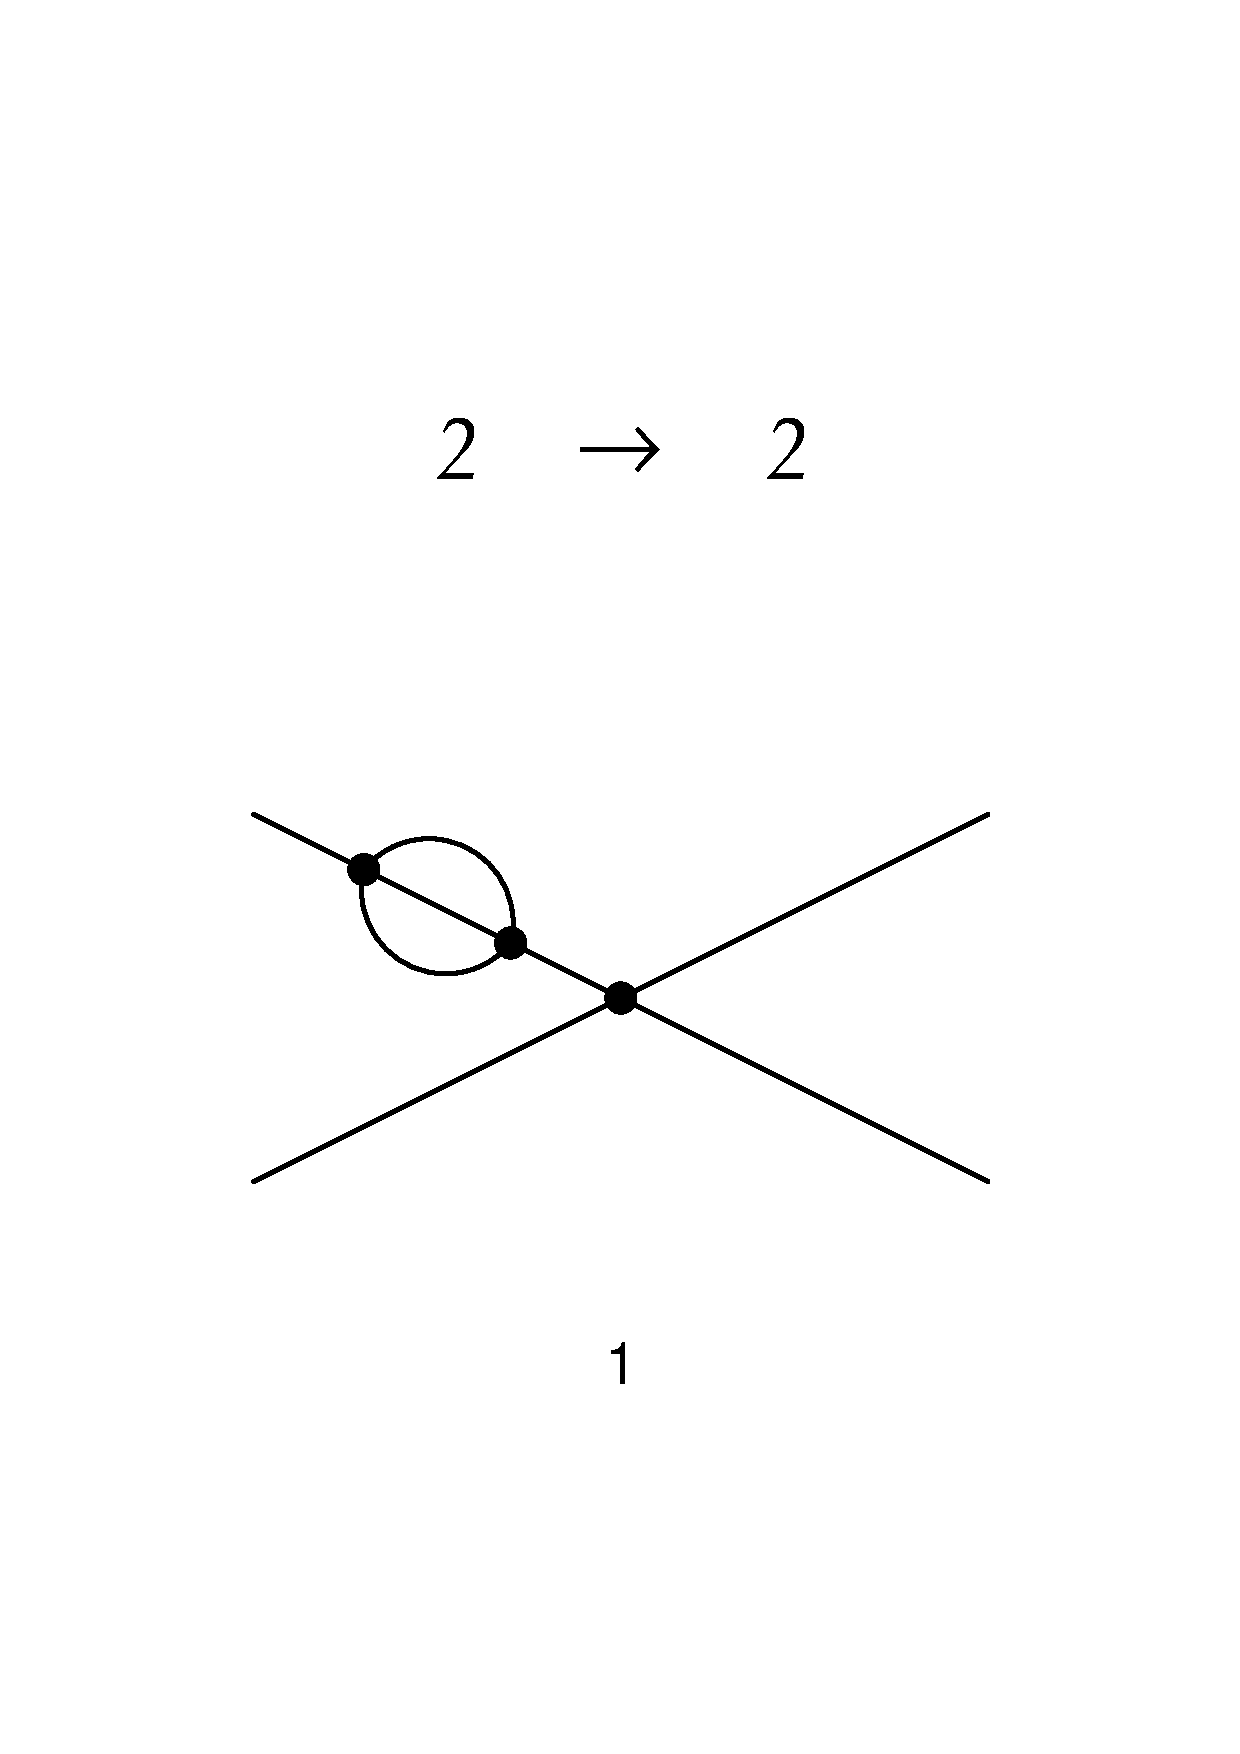
\includegraphics[width=0.28\textwidth]{generated/L2/images/topology39.pdf}
\end{center}
\noindent Parsed propagators: 8. Internal vertices: 3. Internal half-edges: 12.\\
\noindent Assignments checked: 32768. Surviving (nonzero vertex weight): 4096.\\
\noindent Raw $N_c$ power: 0. Net power in $C(t)$: -4.
\[\text{No surviving SK contributions for this topology.}\]
\section*{Topology 40 (FeynArts Topology 6)}
\begin{center}
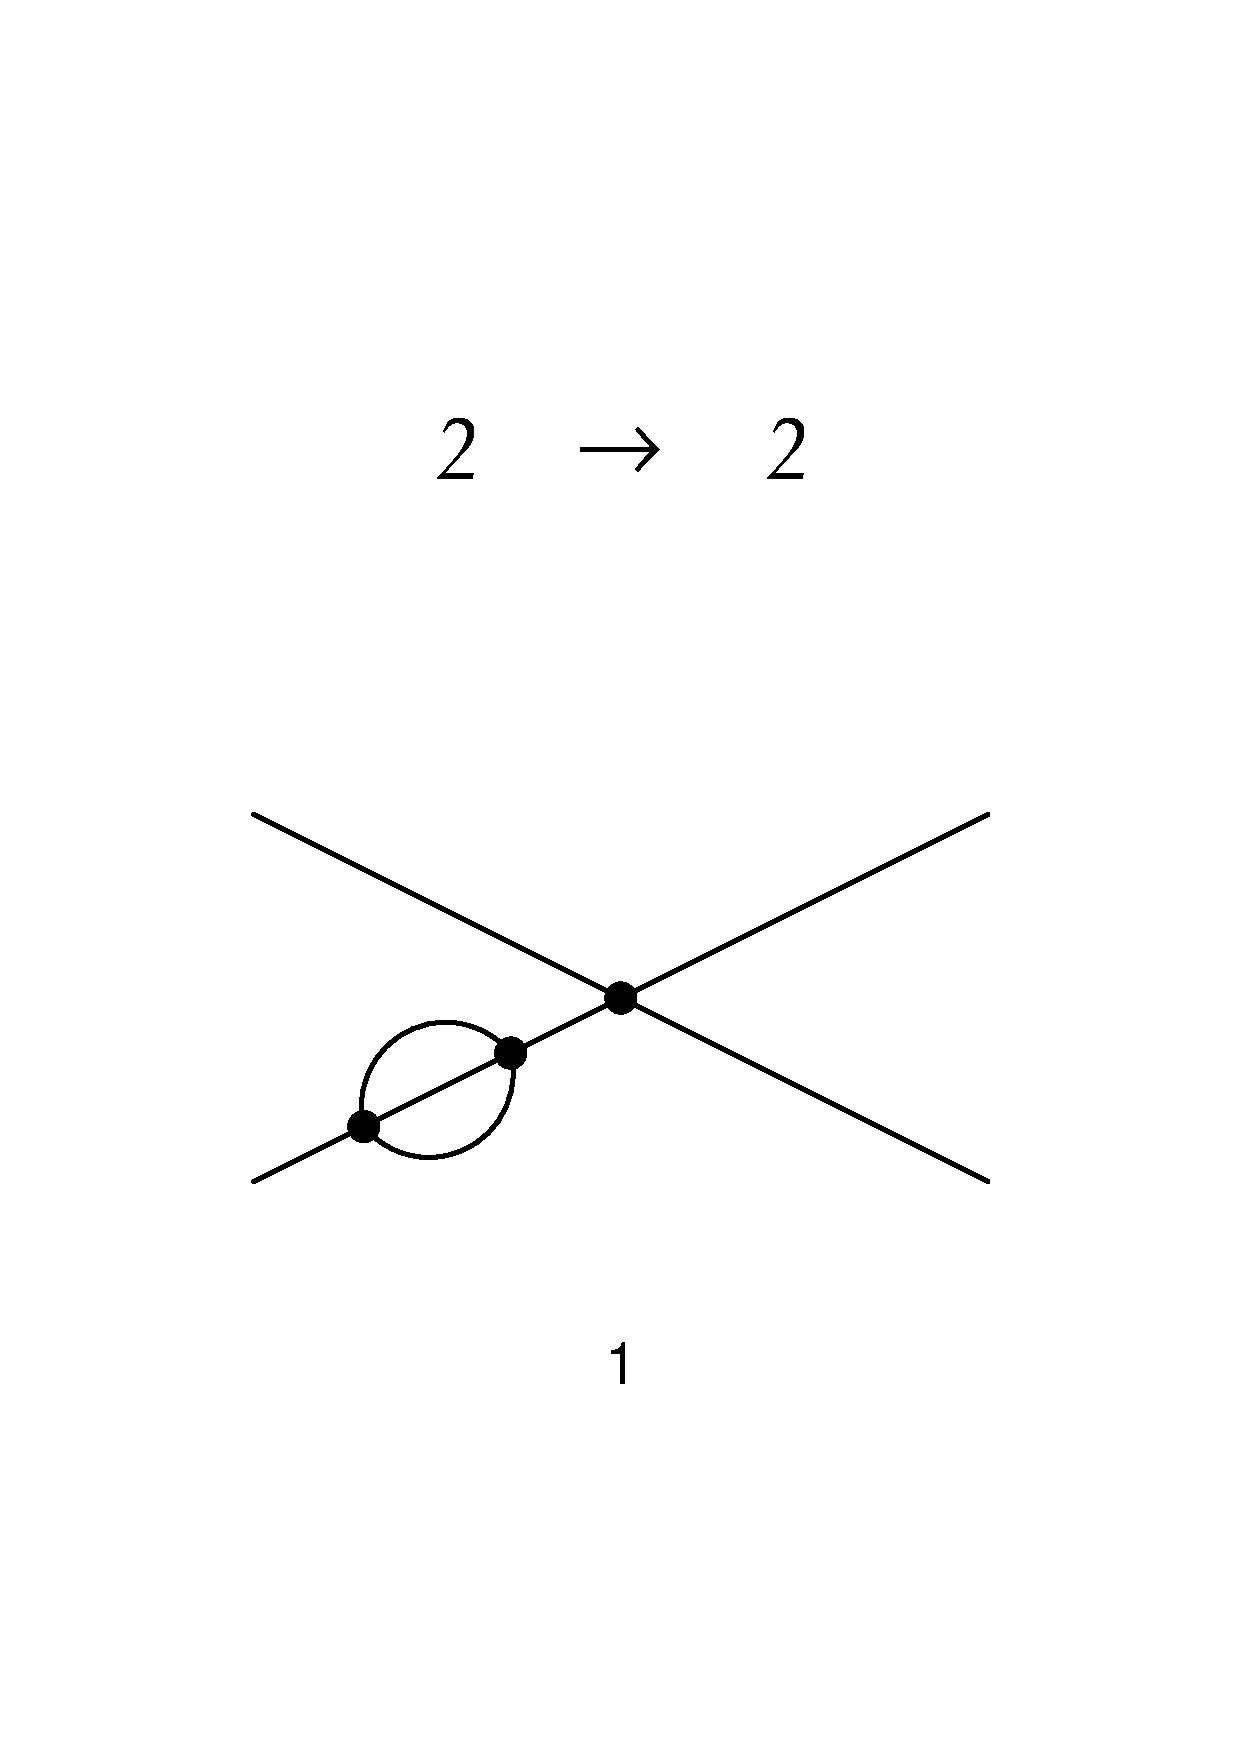
\includegraphics[width=0.28\textwidth]{generated/L2/images/topology40.pdf}
\end{center}
\noindent Parsed propagators: 8. Internal vertices: 3. Internal half-edges: 12.\\
\noindent Assignments checked: 32768. Surviving (nonzero vertex weight): 4096.\\
\noindent Raw $N_c$ power: 0. Net power in $C(t)$: -4.
\noindent Explicit surviving terms:
\begin{equation*}
\mathcal{T}_{40,1} = 384 i g_{2}^{3}\,N_c^{-4}\,G^<\left(x_1,z_{1}\right) \, G^<\left(z_{3},z_{1}\right) \, G_A\left(x_2,z_{2}\right) \, G_A\left(x_4,z_{1}\right) \, G_A\left(z_{3},z_{2}\right) \, G_K\left(z_{3},z_{2}\right) \, G_R\left(x_3,z_{1}\right) \, G_R\left(z_{3},z_{2}\right)
\end{equation*}
\section*{Topology 41 (FeynArts Topology 6)}
\begin{center}
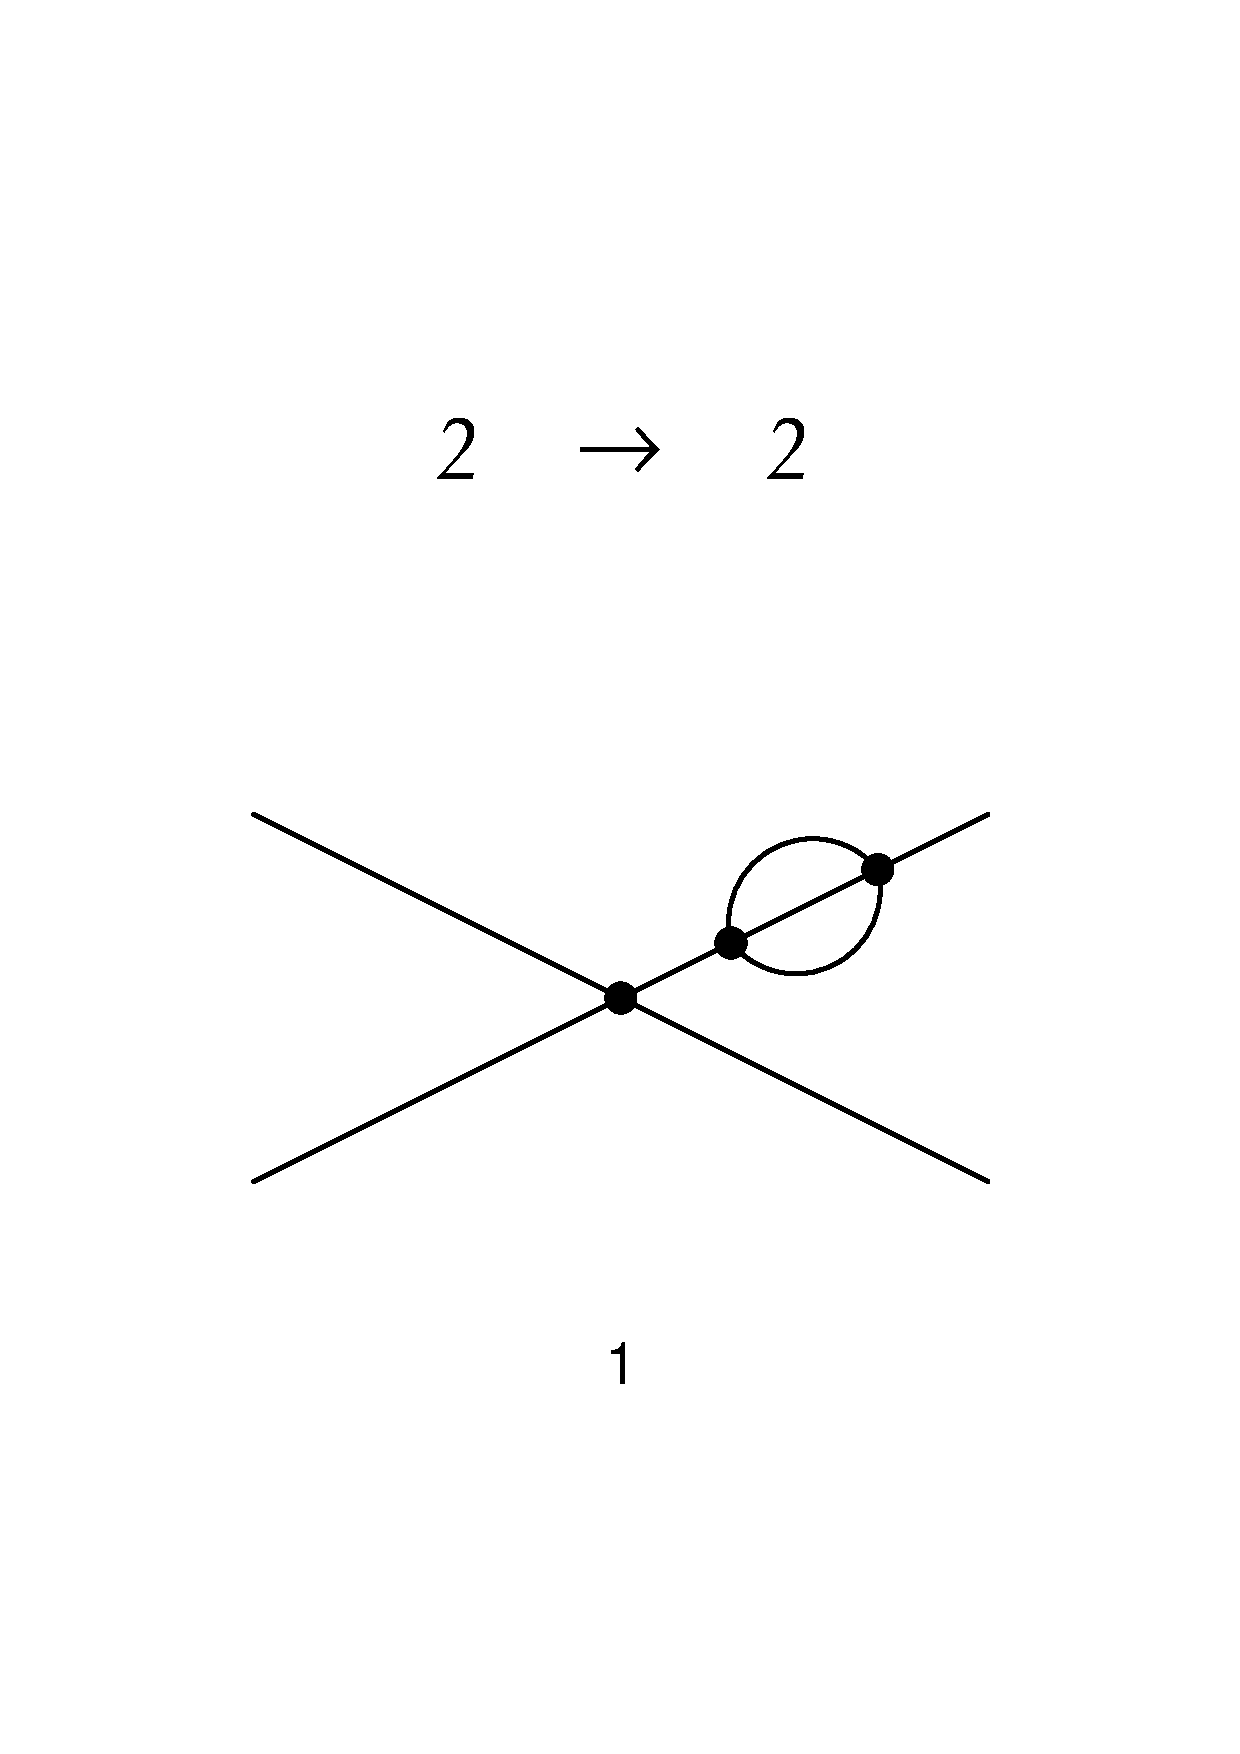
\includegraphics[width=0.28\textwidth]{generated/L2/images/topology41.pdf}
\end{center}
\noindent Parsed propagators: 8. Internal vertices: 3. Internal half-edges: 12.\\
\noindent Assignments checked: 32768. Surviving (nonzero vertex weight): 4096.\\
\noindent Raw $N_c$ power: 0. Net power in $C(t)$: -4.
\[\text{No surviving SK contributions for this topology.}\]
\section*{Topology 42 (FeynArts Topology 6)}
\begin{center}
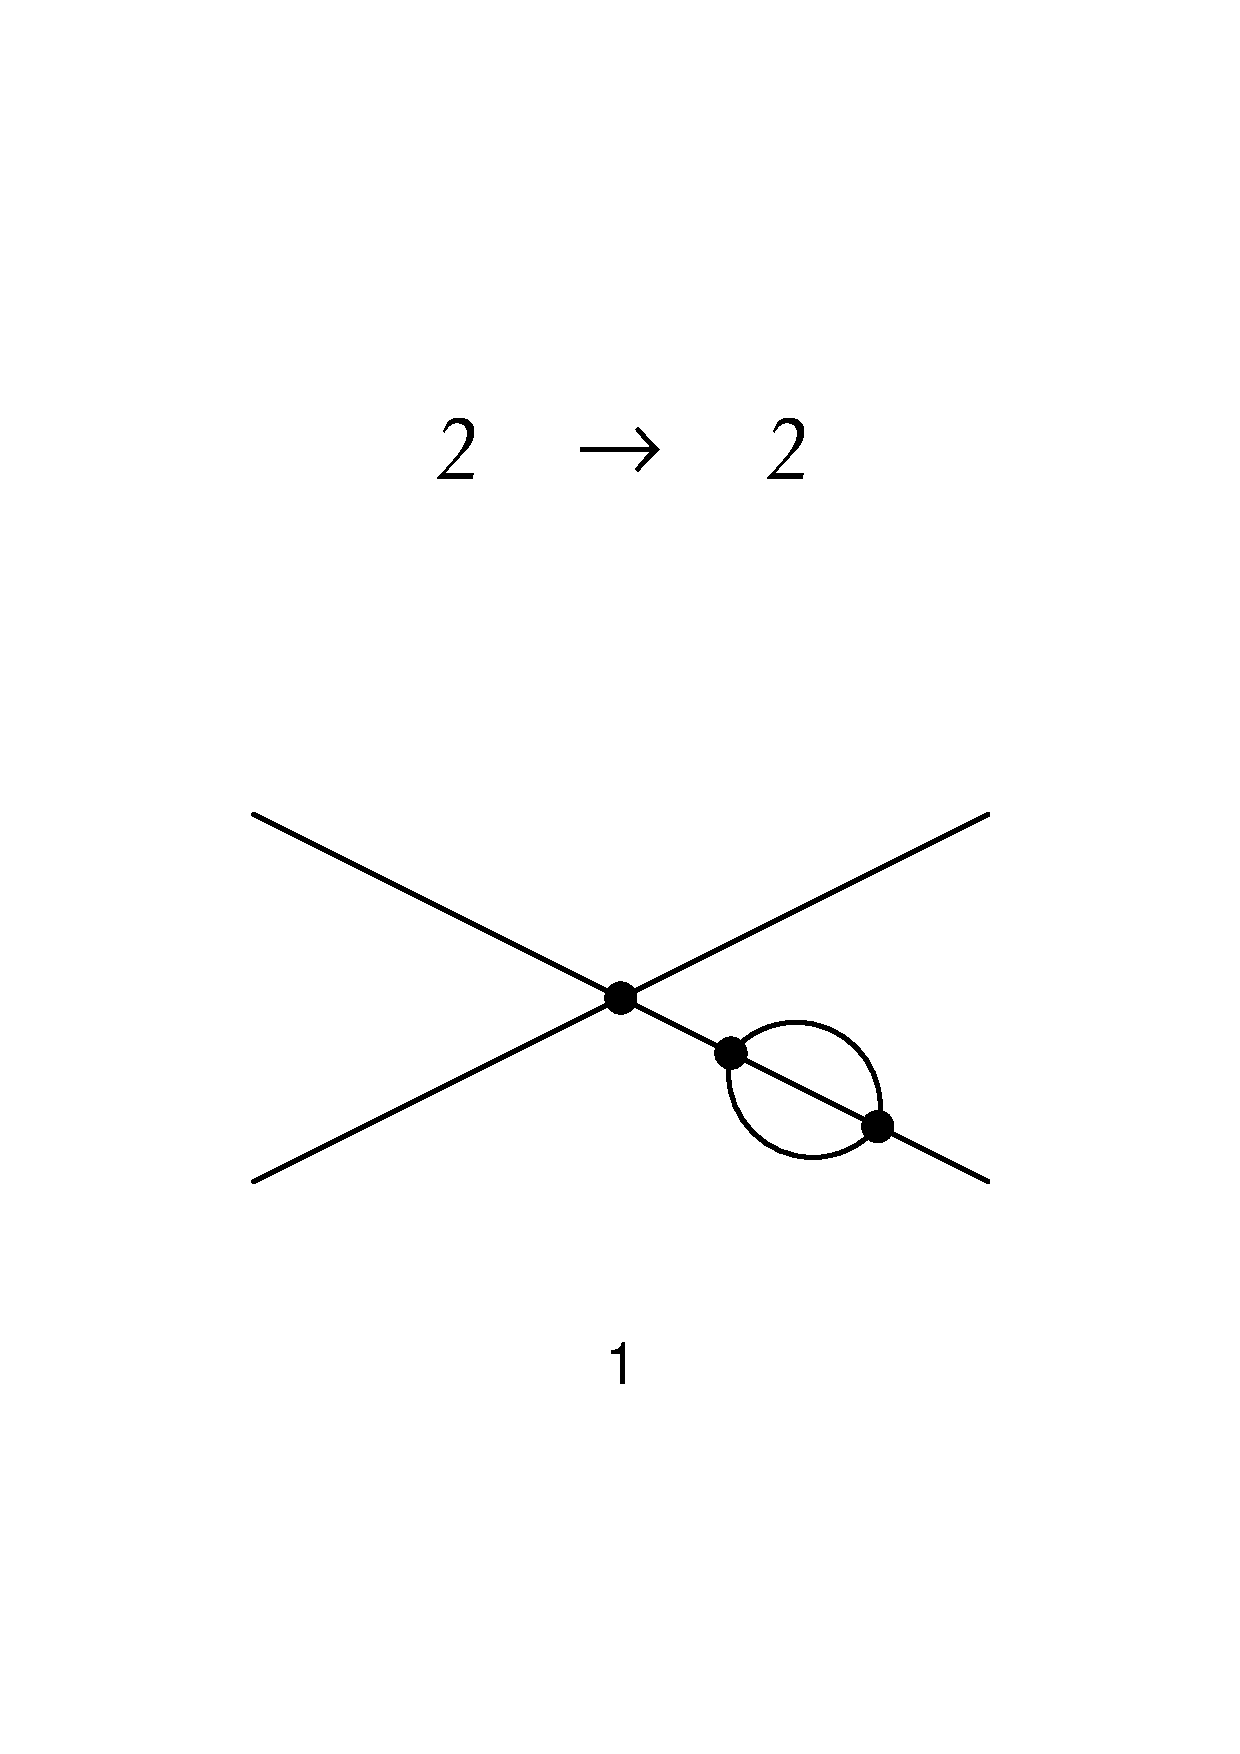
\includegraphics[width=0.28\textwidth]{generated/L2/images/topology42.pdf}
\end{center}
\noindent Parsed propagators: 8. Internal vertices: 3. Internal half-edges: 12.\\
\noindent Assignments checked: 32768. Surviving (nonzero vertex weight): 4096.\\
\noindent Raw $N_c$ power: 0. Net power in $C(t)$: -4.
\noindent Explicit surviving terms:
\begin{equation*}
\mathcal{T}_{42,1} = 384 i g_{2}^{3}\,N_c^{-4}\,G^>\left(x_3,z_{1}\right) \, G^>\left(z_{3},z_{1}\right) \, G_A\left(x_2,z_{1}\right) \, G_A\left(x_4,z_{2}\right) \, G_A\left(z_{3},z_{2}\right) \, G_K\left(z_{3},z_{2}\right) \, G_R\left(x_1,z_{1}\right) \, G_R\left(z_{3},z_{2}\right)
\end{equation*}
\end{document}